\documentclass{article}
\usepackage[utf8]{inputenc}
\usepackage{graphicx}
\usepackage{enumerate}
\usepackage{amsmath}

\graphicspath{{../figs/}}

\setlength{\parindent}{4em}
\setlength{\parskip}{1em}
\renewcommand{\baselinestretch}{1.3}

\makeatletter
% we use \prefix@<level> only if it is defined
\renewcommand{\seccntformat}[1]{%
  \ifcsname prefix@#1\endcsname
    \csname prefix@#1\endcsname
  \else
    \csname the#1\endcsname\quad
  \fi}
% define \prefix@section
\newcommand\prefix@section{Part \thesection: }
\makeatother

\title{Lab05: Snowball Earth: Diffusion Equation}
\author{Prithvi Thakur}
\date{Nov 22, 2018}

\begin{document}

\maketitle

% Problem 1
\section*{Discretize the purely diffusive part of the differential equation}
We discretize the diffusion equation and construct the second derivative finite difference operator K. We have a zero slope boundary condition on the two ends of our one-dimensional model, and therefore,   we incorporate these first derivative equations as the top and bottom rows in our finite difference matrix K.

We test this diffusive part of the equation with a simple temperature function varying sinusoidally with the latitude, given by $T(\phi) = \sin(\phi)$, where $\phi$ is the latiude in radians, and $T$ is the temperature.
\begin{figure}
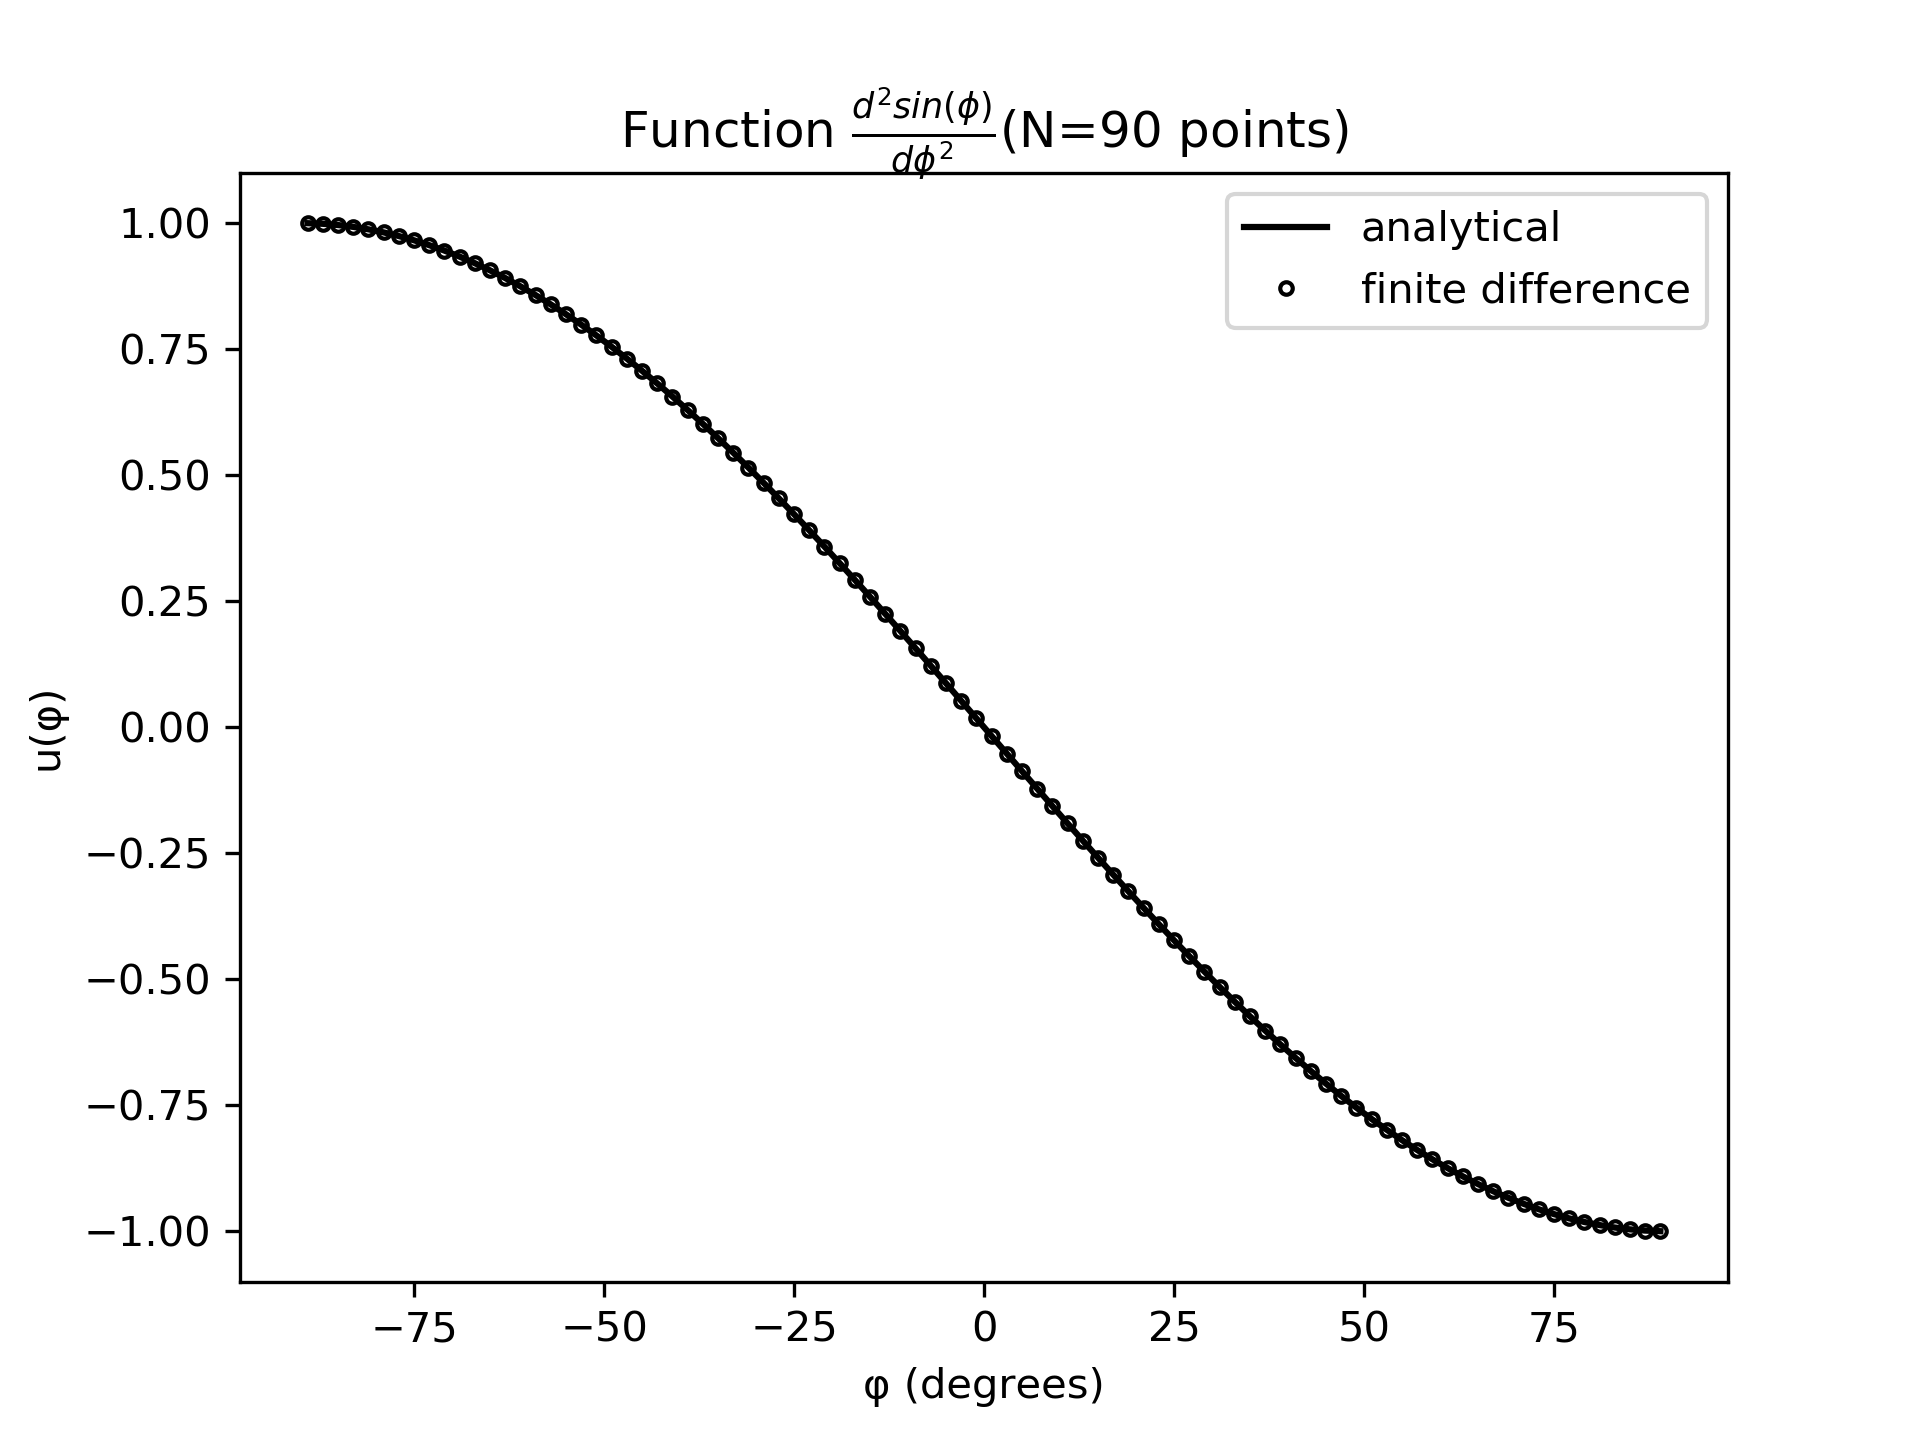
\includegraphics[scale=0.6]{diffusive_part.png}
\caption{Testing the diffusive part of the discretized pde against analytical solution}
\end{figure}

% Problem 2
\section*{Discretize the area term as an external forcing}
As described in step 3, we discretize the area term in the diffusion equation and use appropriate neumann boundary conditions to modify the right hand side of our matrix equation. We compare it using analytical solution with the following assumed values.
\begin{aligned}
    T &= \sin(\phi) \\
    A &= R_e\phi^2 + R_e \\
    \frac{dT}{dt} &= \lambda(\frac{-\sin(\phi)}{R_e^2} + \frac{2\phi\cos\phi}{R_e^2(\phi^2 + 1)})
\end{aligned}

\begin{figure}
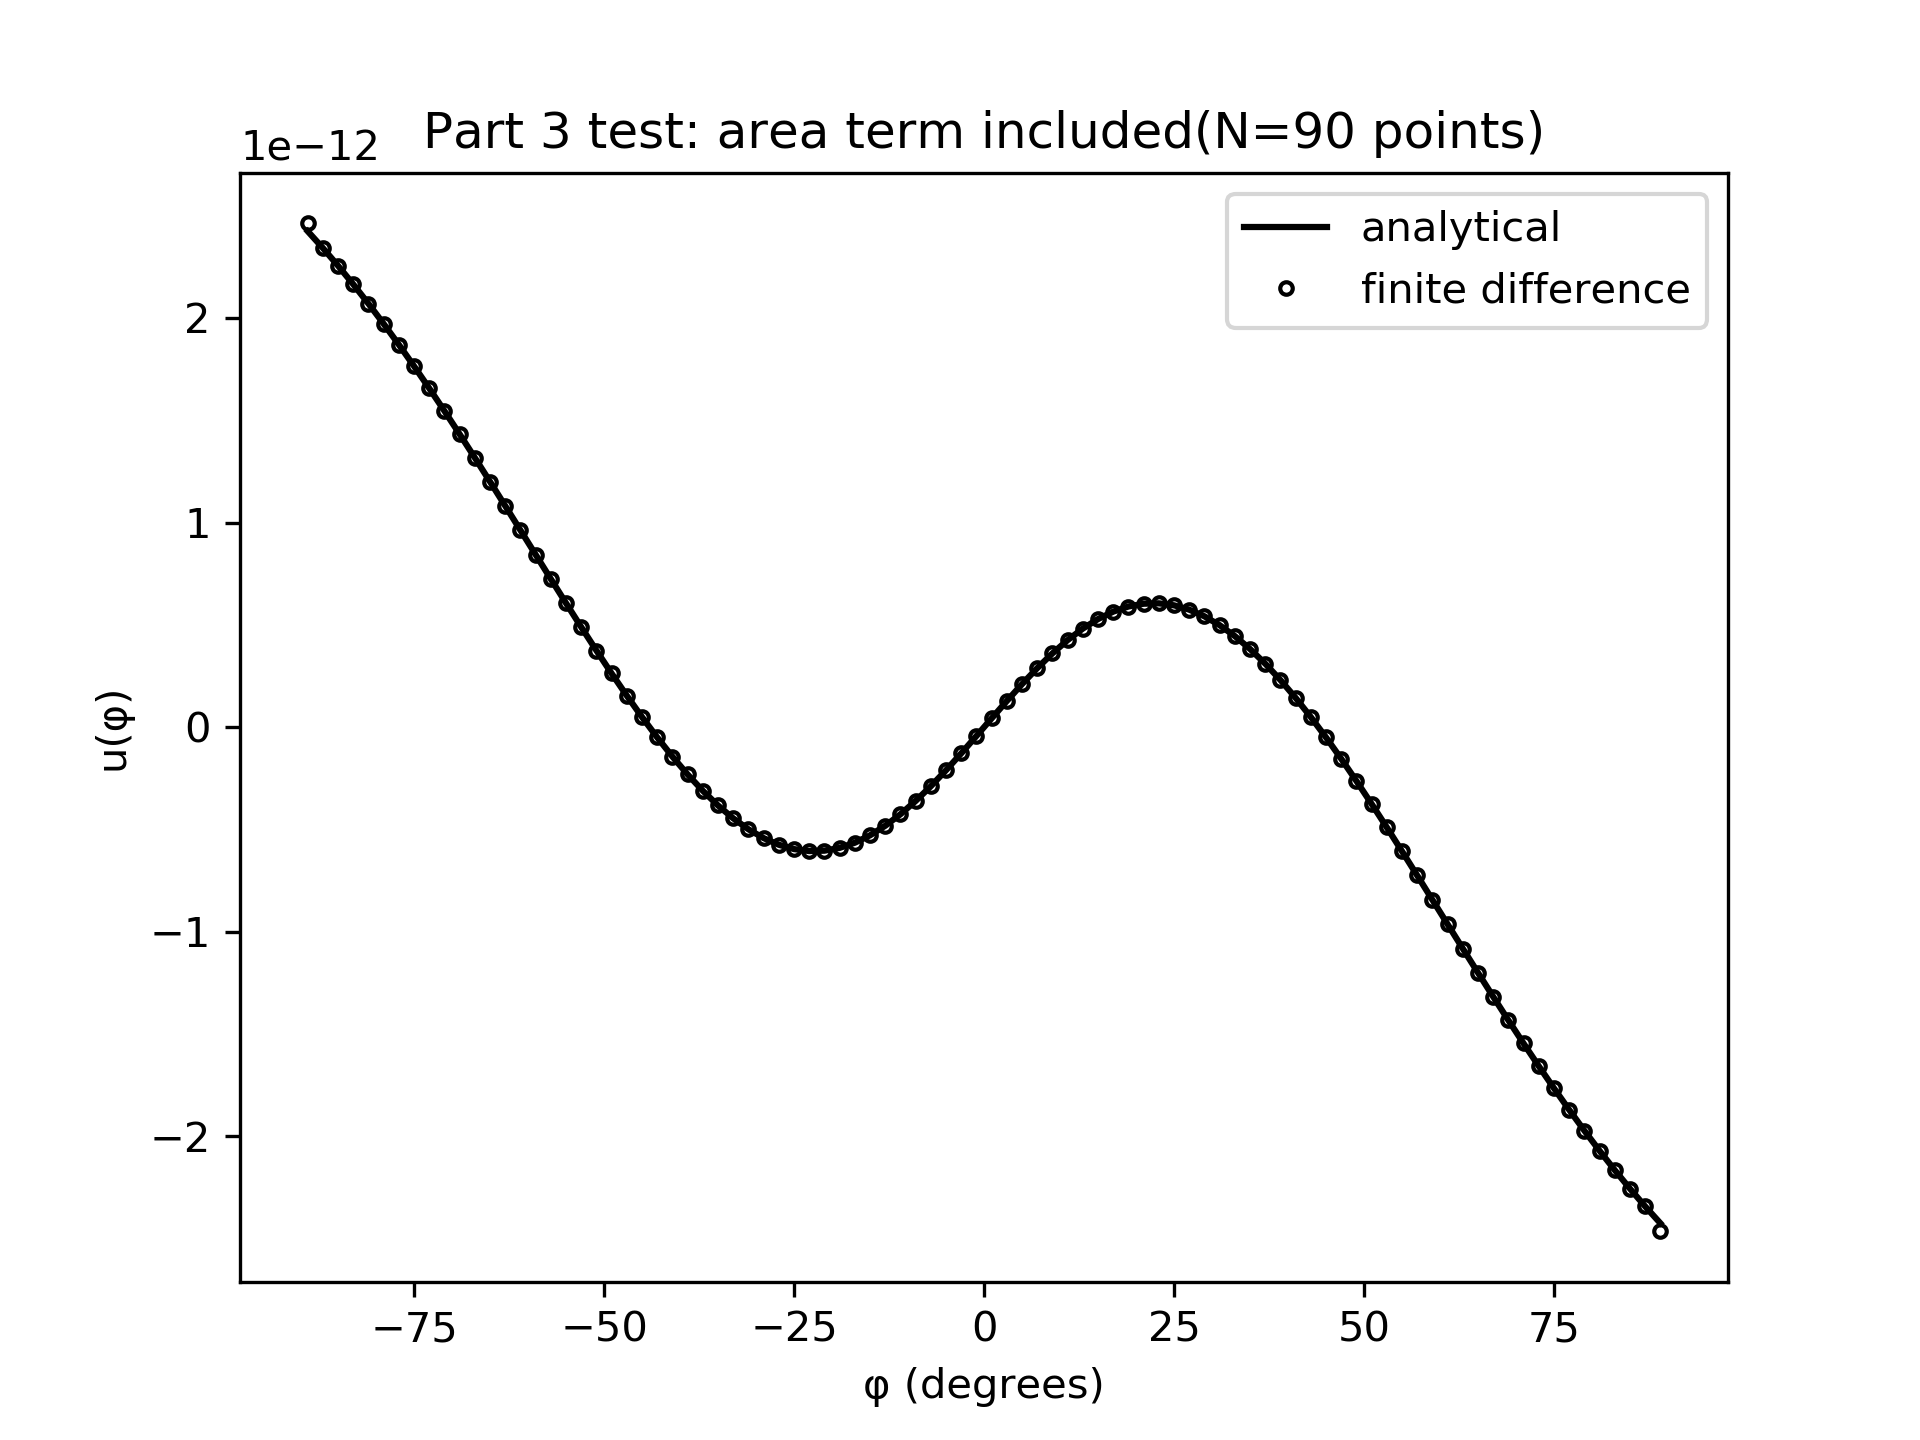
\includegraphics[scale=0.6]{part3.png}
\caption{Testing with the area term included as forcing.}
\end{figure}


% Problem 3
\section*{Question 0}
We tested the diffusive and area term of the differential equations against known analytical solutions. This test combined with the resolution test (no change in solution upon mesh refinement) are sufficient tests to prove the working of the code. The tests for timestepping process is similar to the output in question 1. We will see that since the mean temperature is not dropping by very high values, the steady state solution is stable.


\section*{Question 1}
In the steady state solution, temperature of all the latitudes converge to same temperature after sufficient time (Fig. 3). If we look at the global average temperature variation through time, we see that it doesn't vary more than 0..6-0.8 degrees celsius throughout. For our computational accurary, we can say that the total temperature is conserved.

\begin{figure}
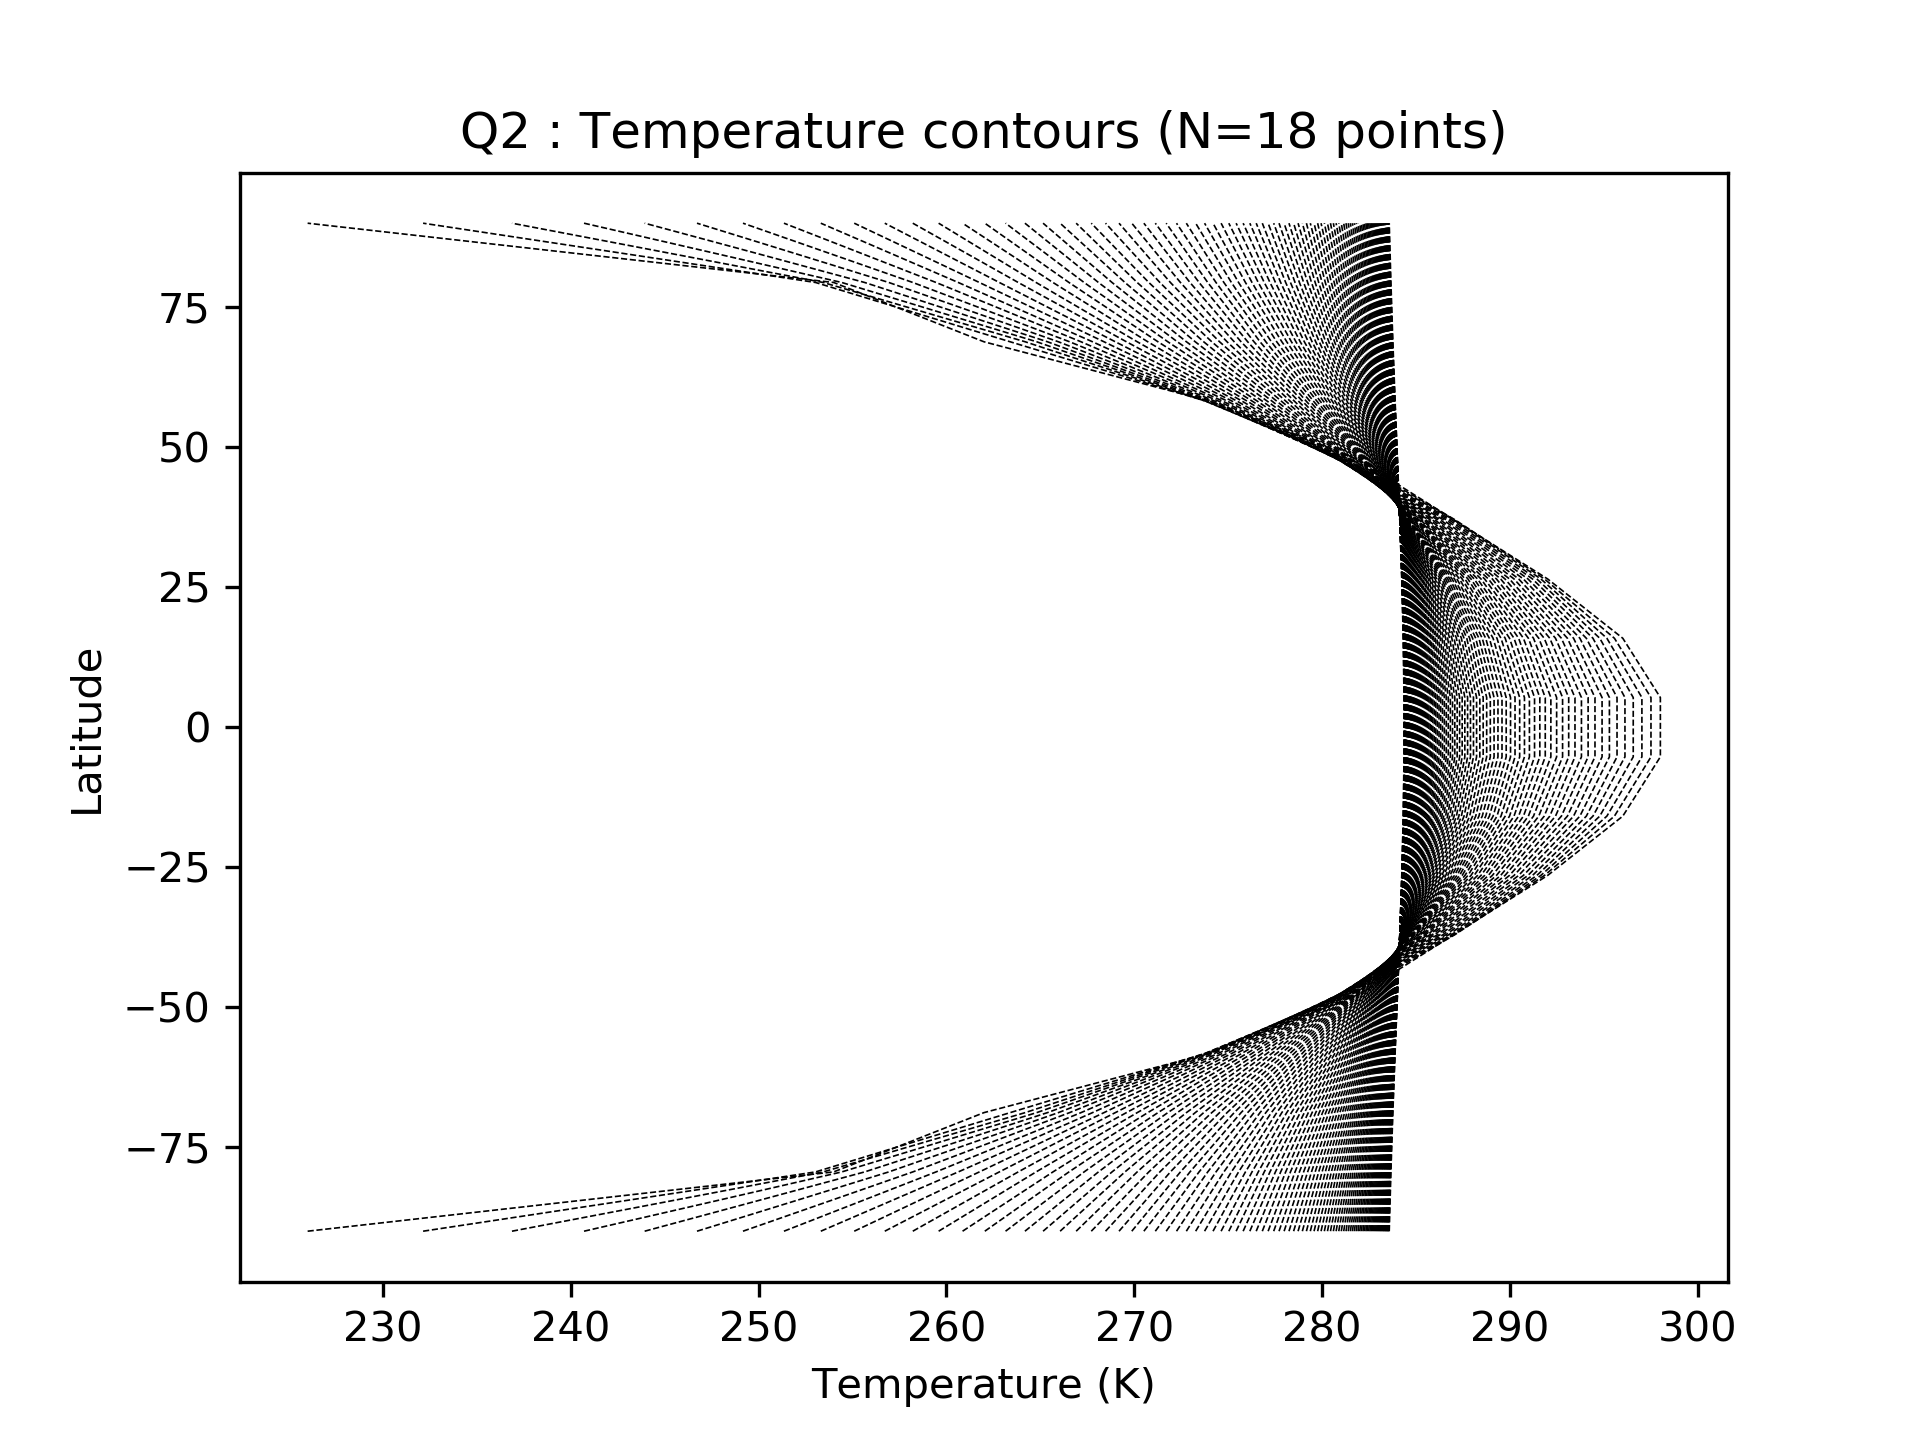
\includegraphics[scale=0.7]{tcont_q1.png} 
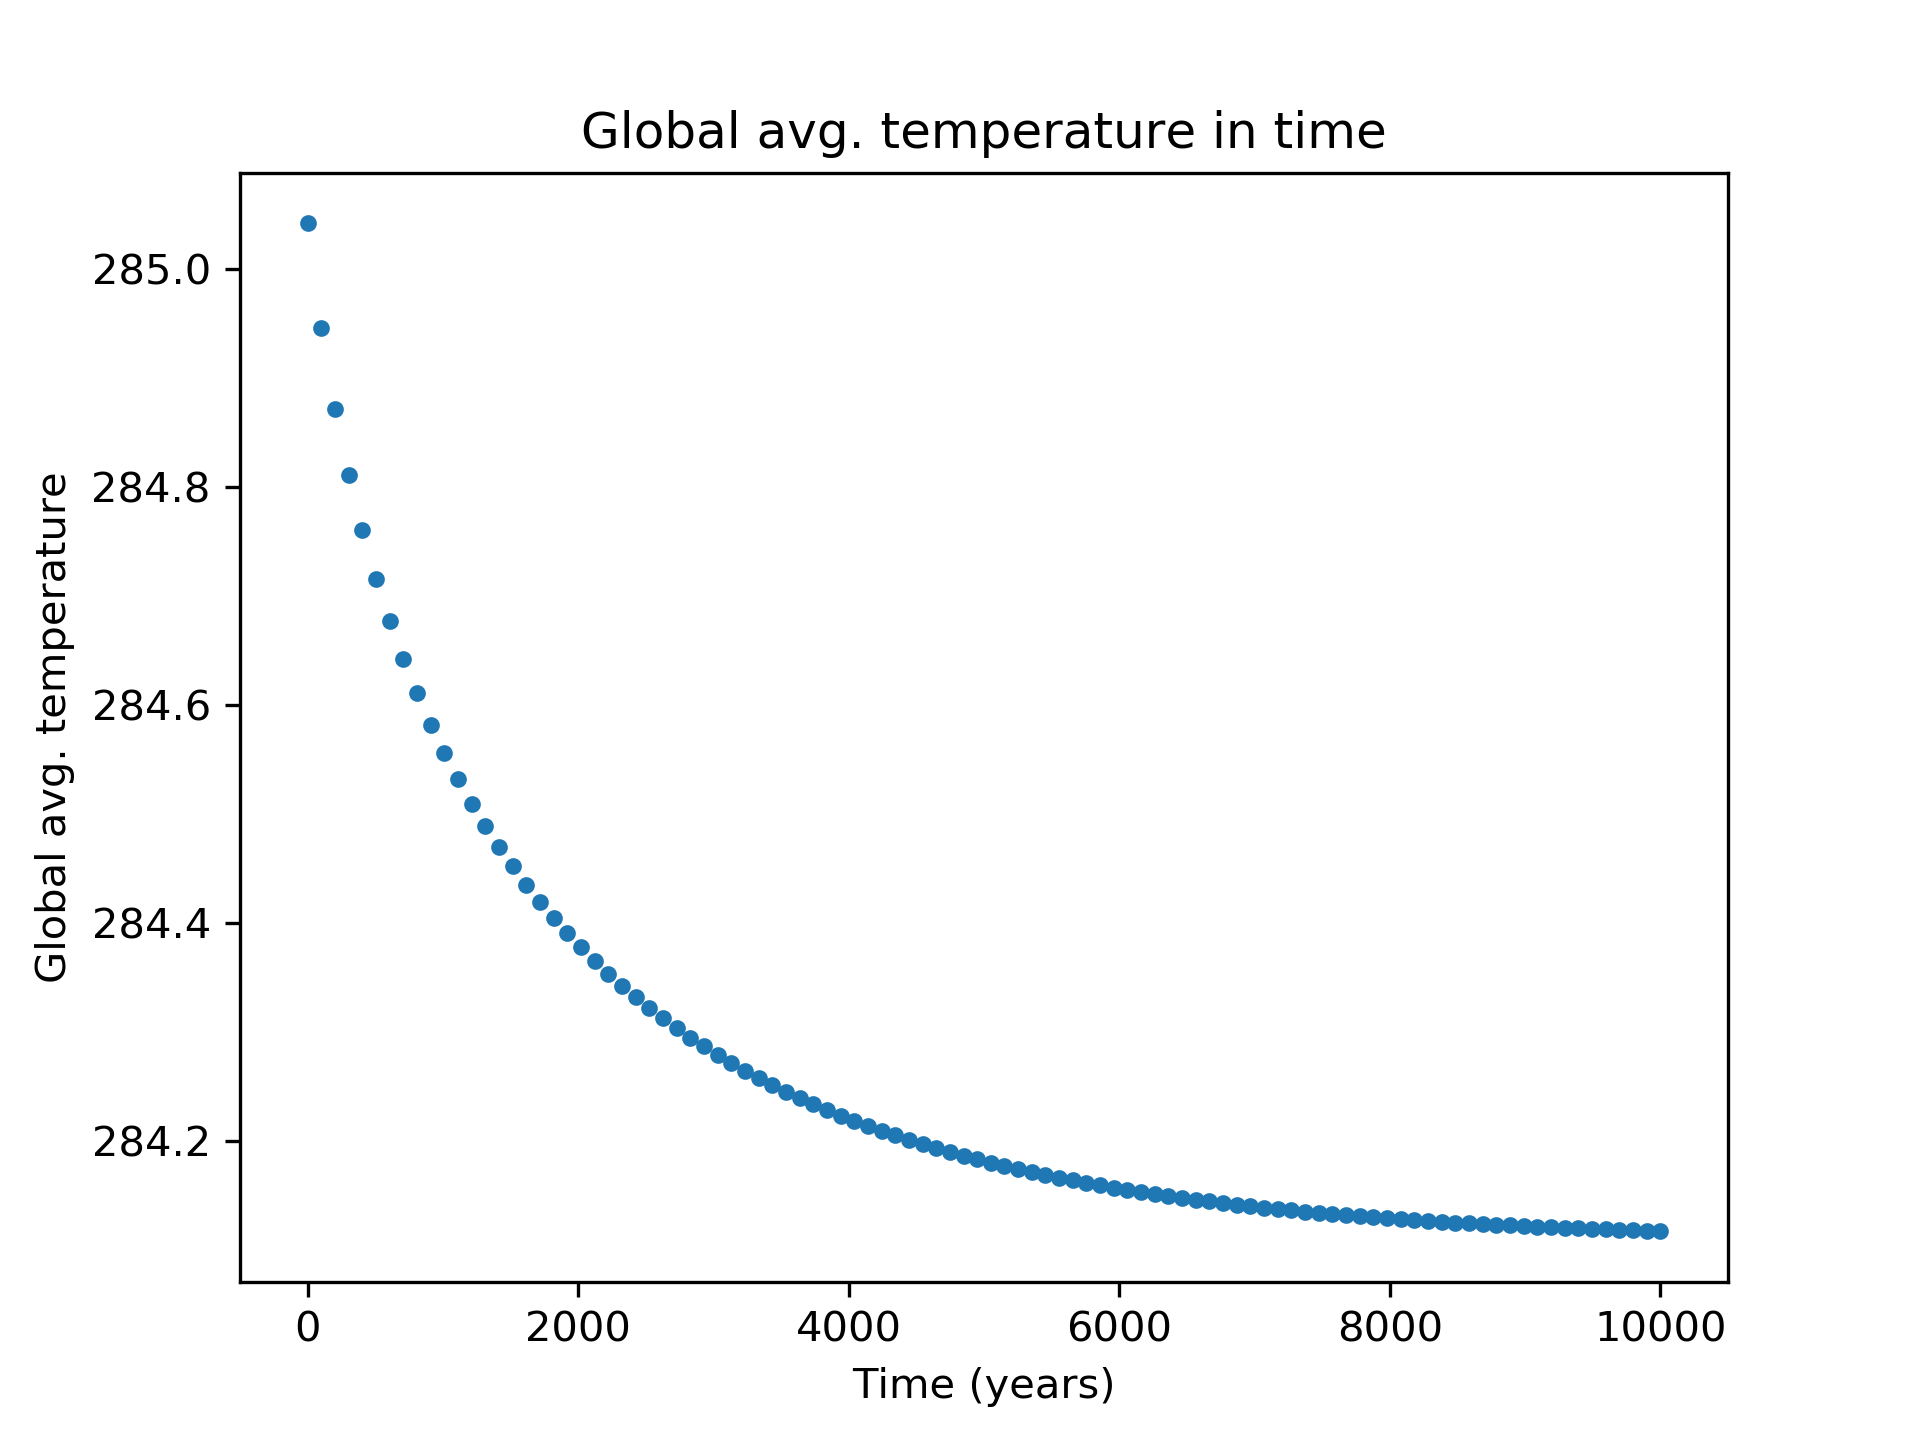
\includegraphics[scale=0.7]{tavg_q1.png}
\caption{Temperature isolines and the global average steady state temperature}
\end{figure}

\section*{Question 2}
We add solar insolation terms and see the temperature contours in Fig. 4. We see that the poles do not heat up as fast as in figure 3, rather every band seems to increase uniformly. Fig. 5 shows the variation in diffusivity on the steady state temperature distribution. The diffusivity is varied from $10-100 m^2s^{-1}$ and we see that the higer diffusivity will tend to homogenize the temperature different across latitudes very quickly.
Higer diffusivity reaches steady state much faster than lower diffusivity.

\begin{figure}
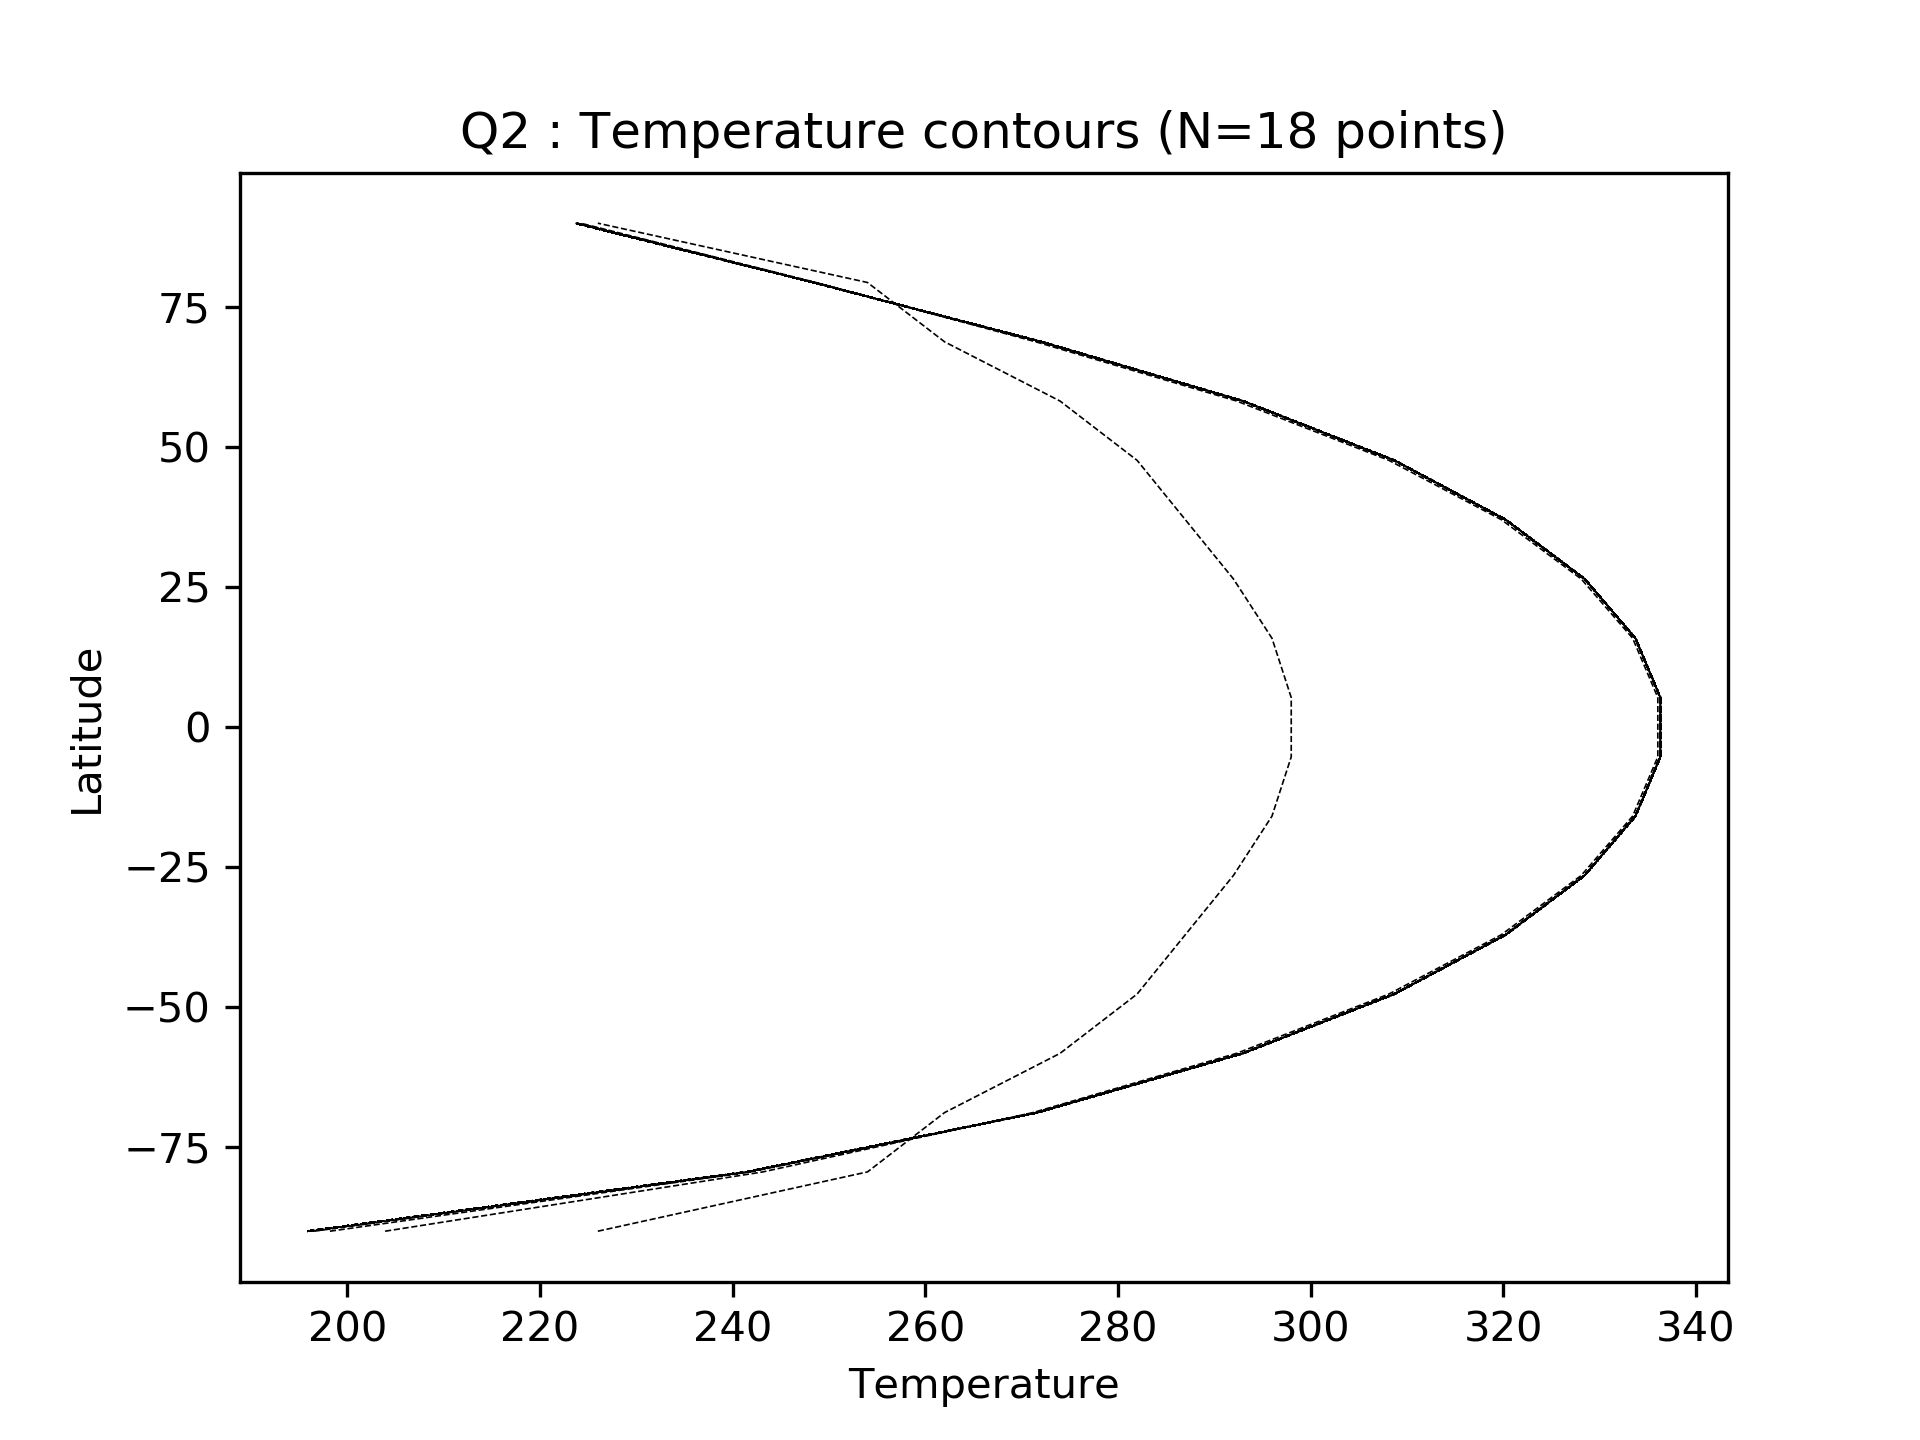
\includegraphics[scale=0.7]{tcont_q2.png} 
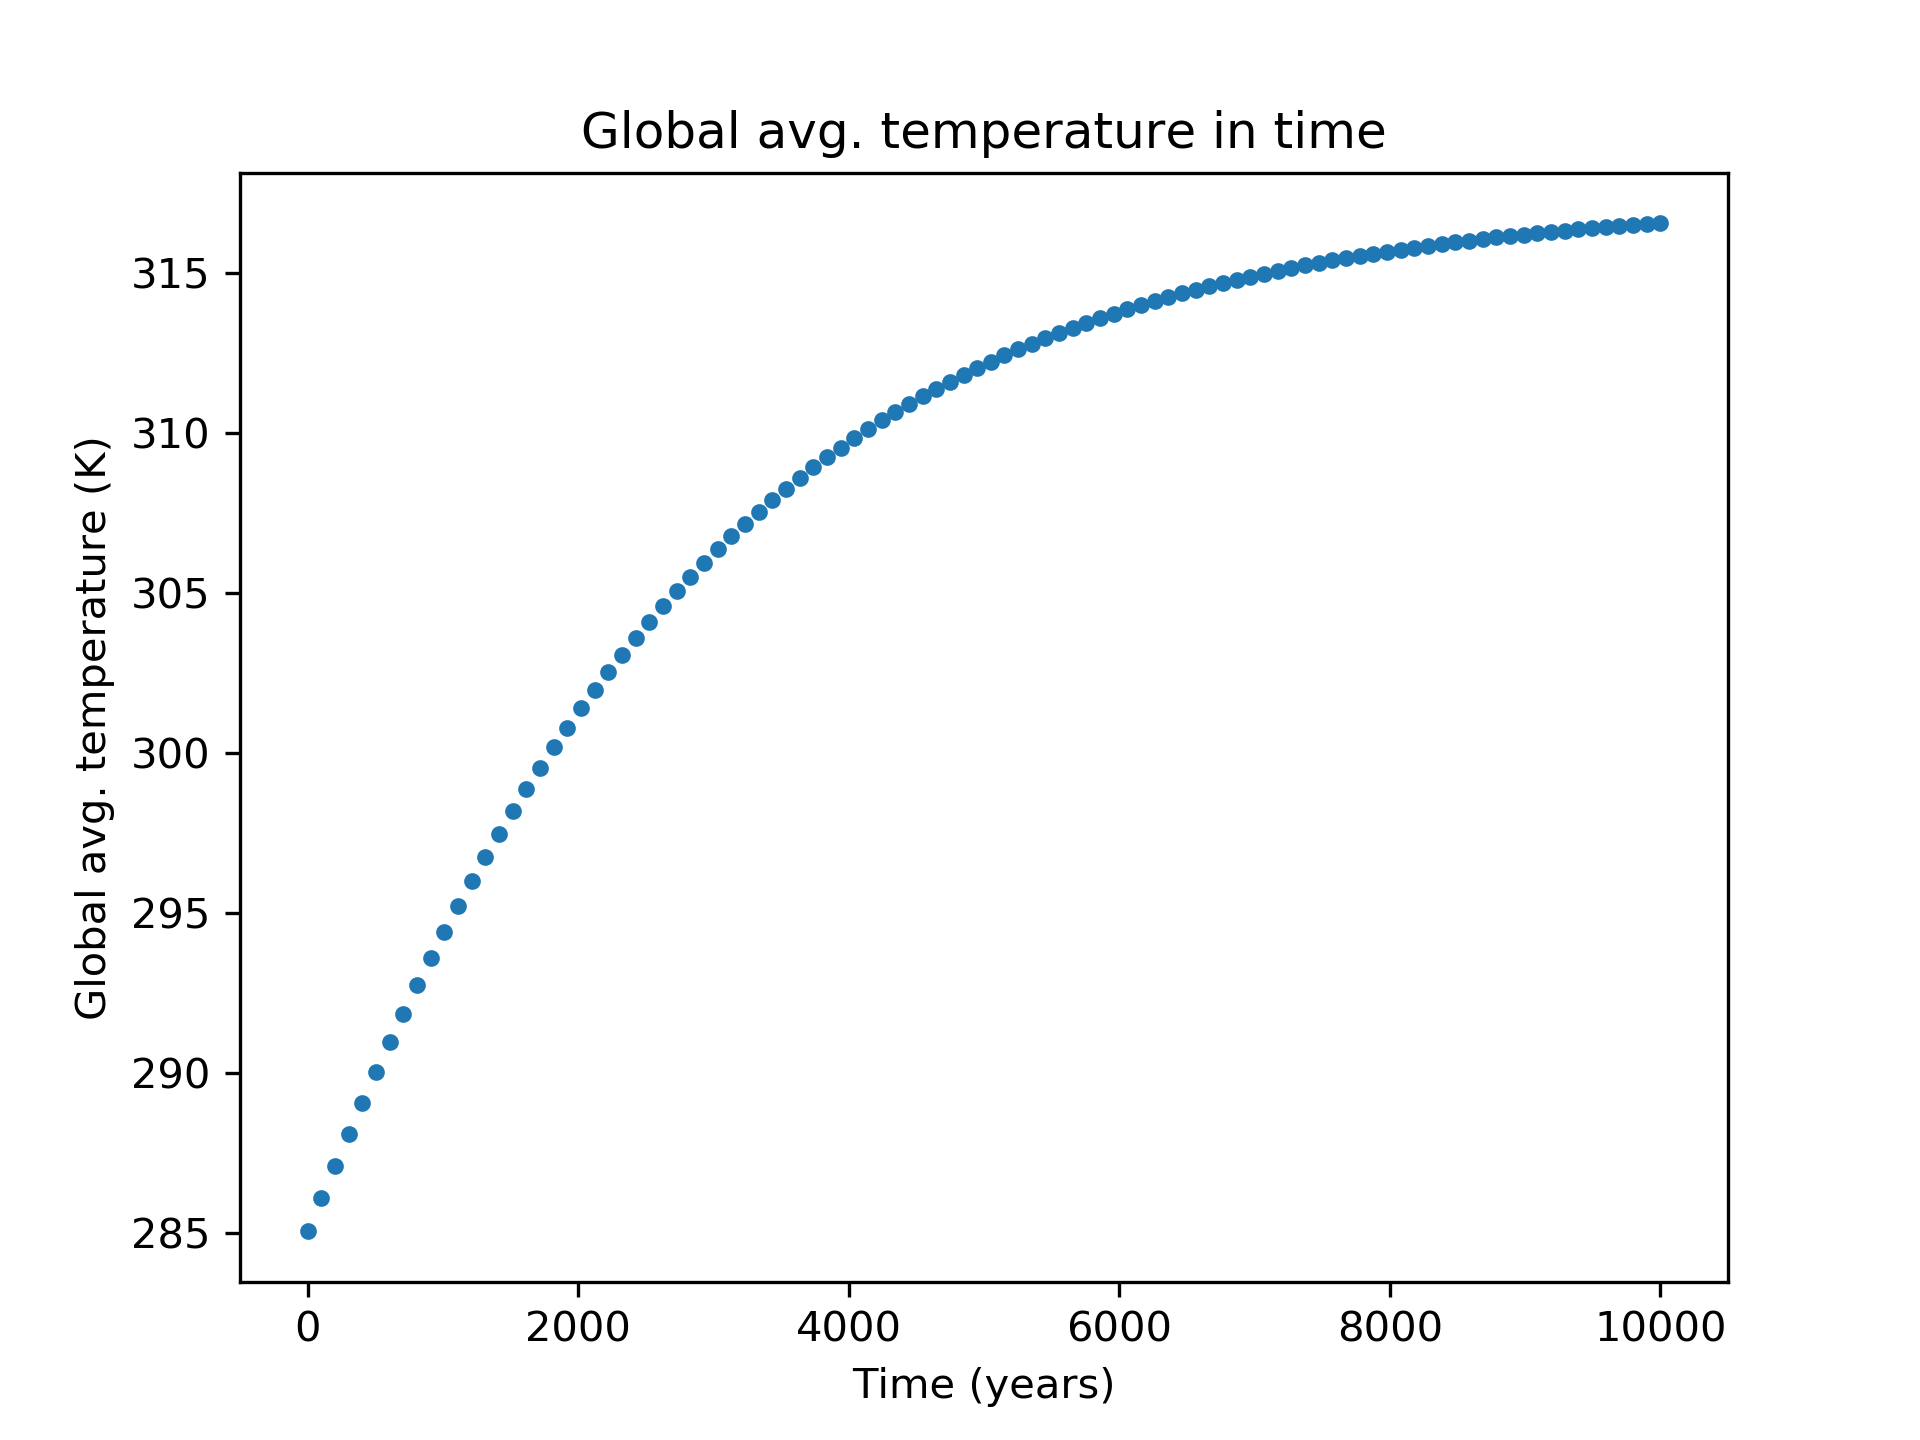
\includegraphics[scale=0.7]{tavg_q2.png}
\caption{Global steady state solution for added insolation terms}
\end{figure}

\begin{figure}
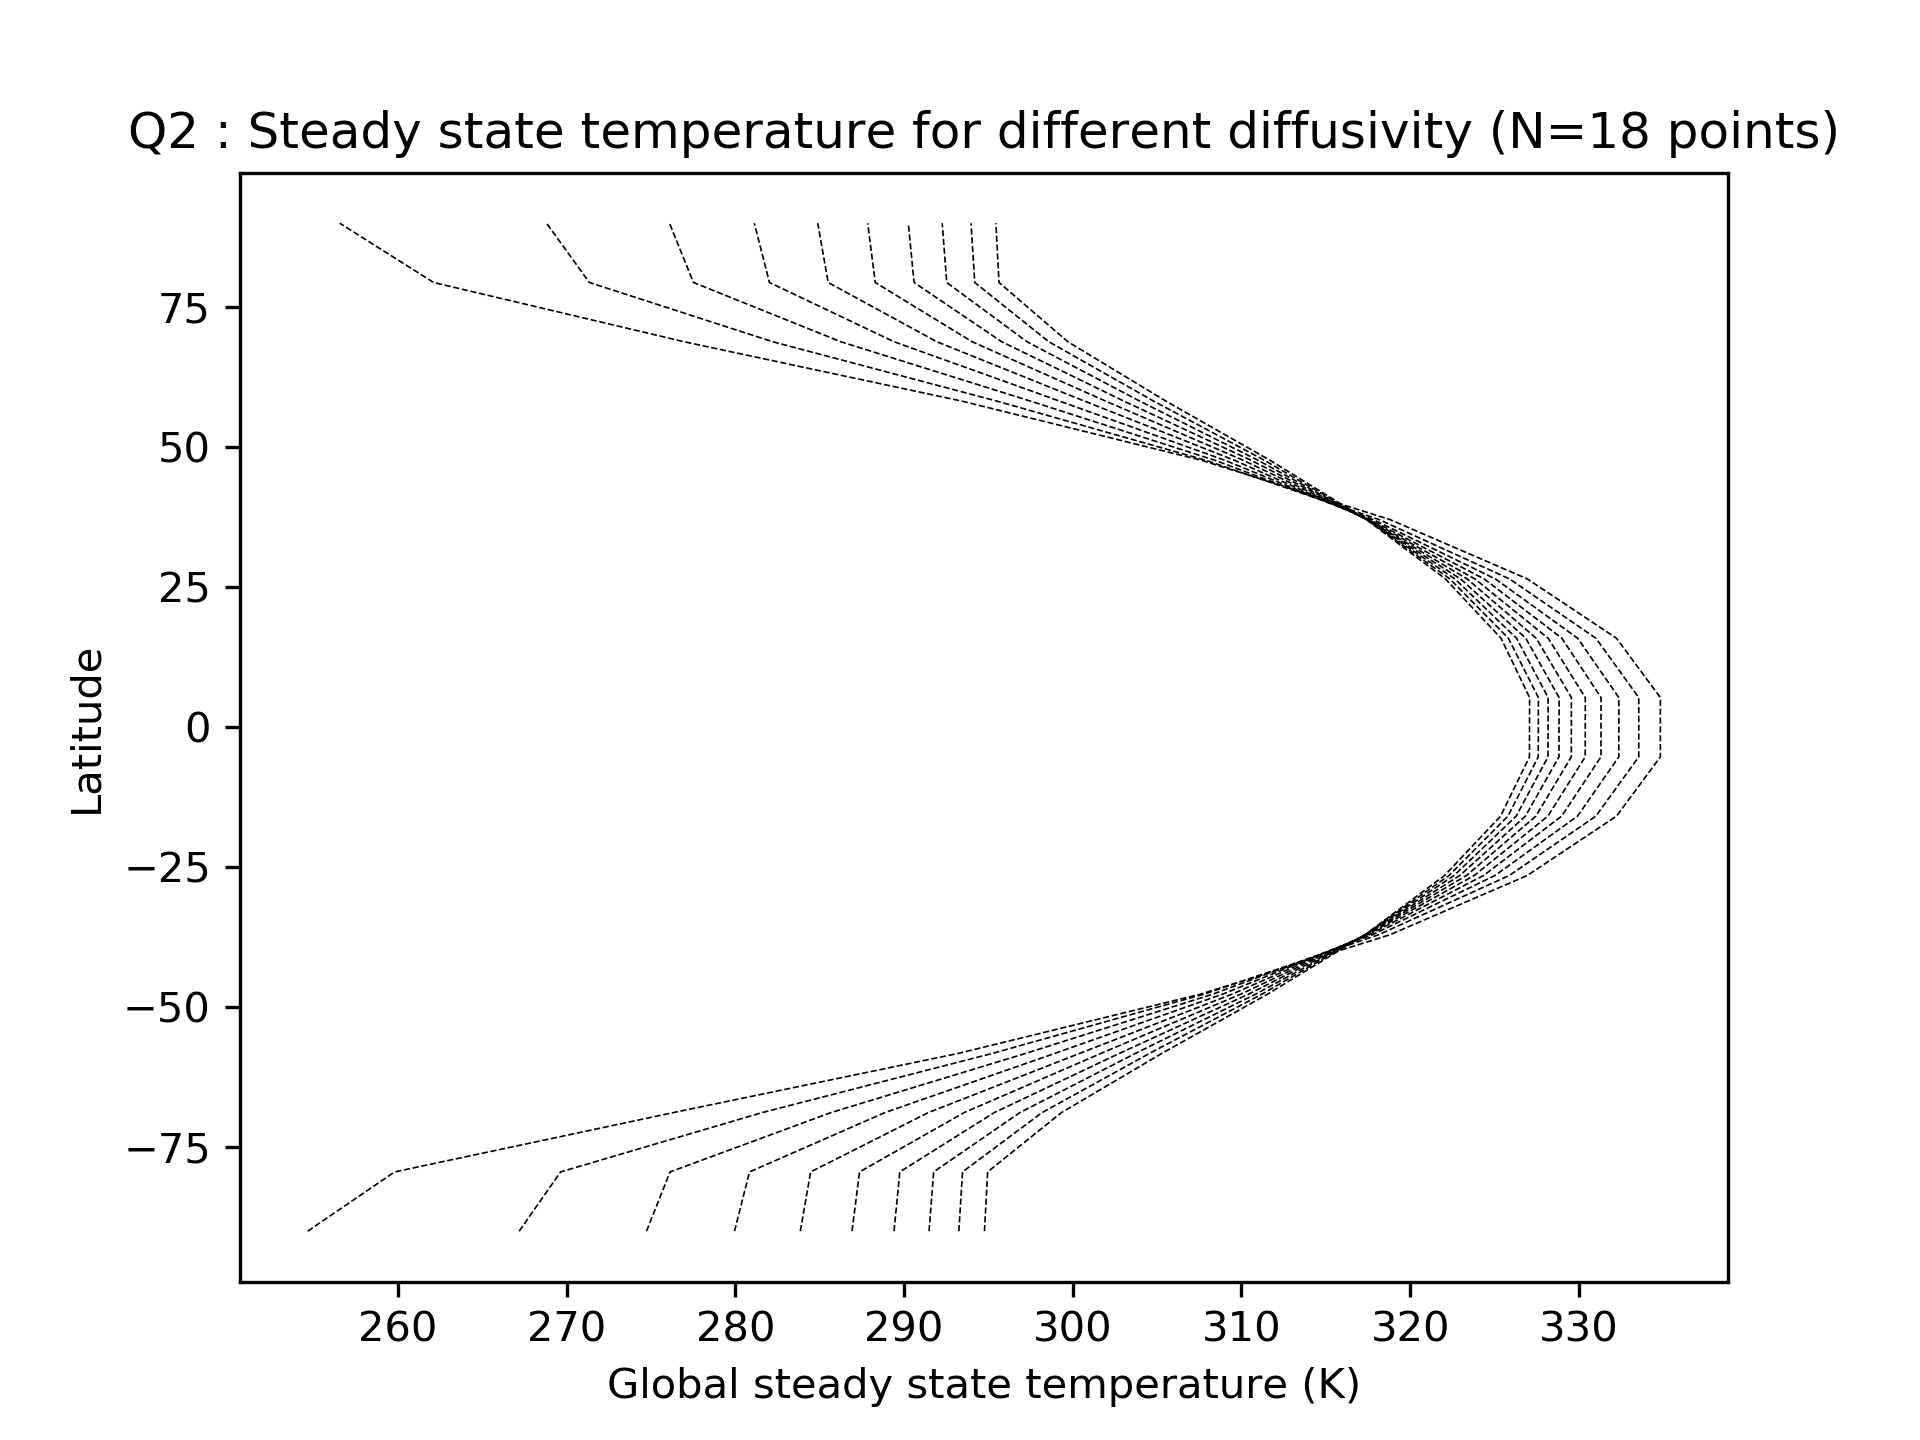
\includegraphics[scale=0.7]{tdiff_q2b.png} 
\caption{Variation in diffusivity for different simulations. The diffusivity varies from 10 to 100 in increments of 10. The one with the highest temperature at equators is the lowest diffusivity.}
\end{figure}

\begin{figure}
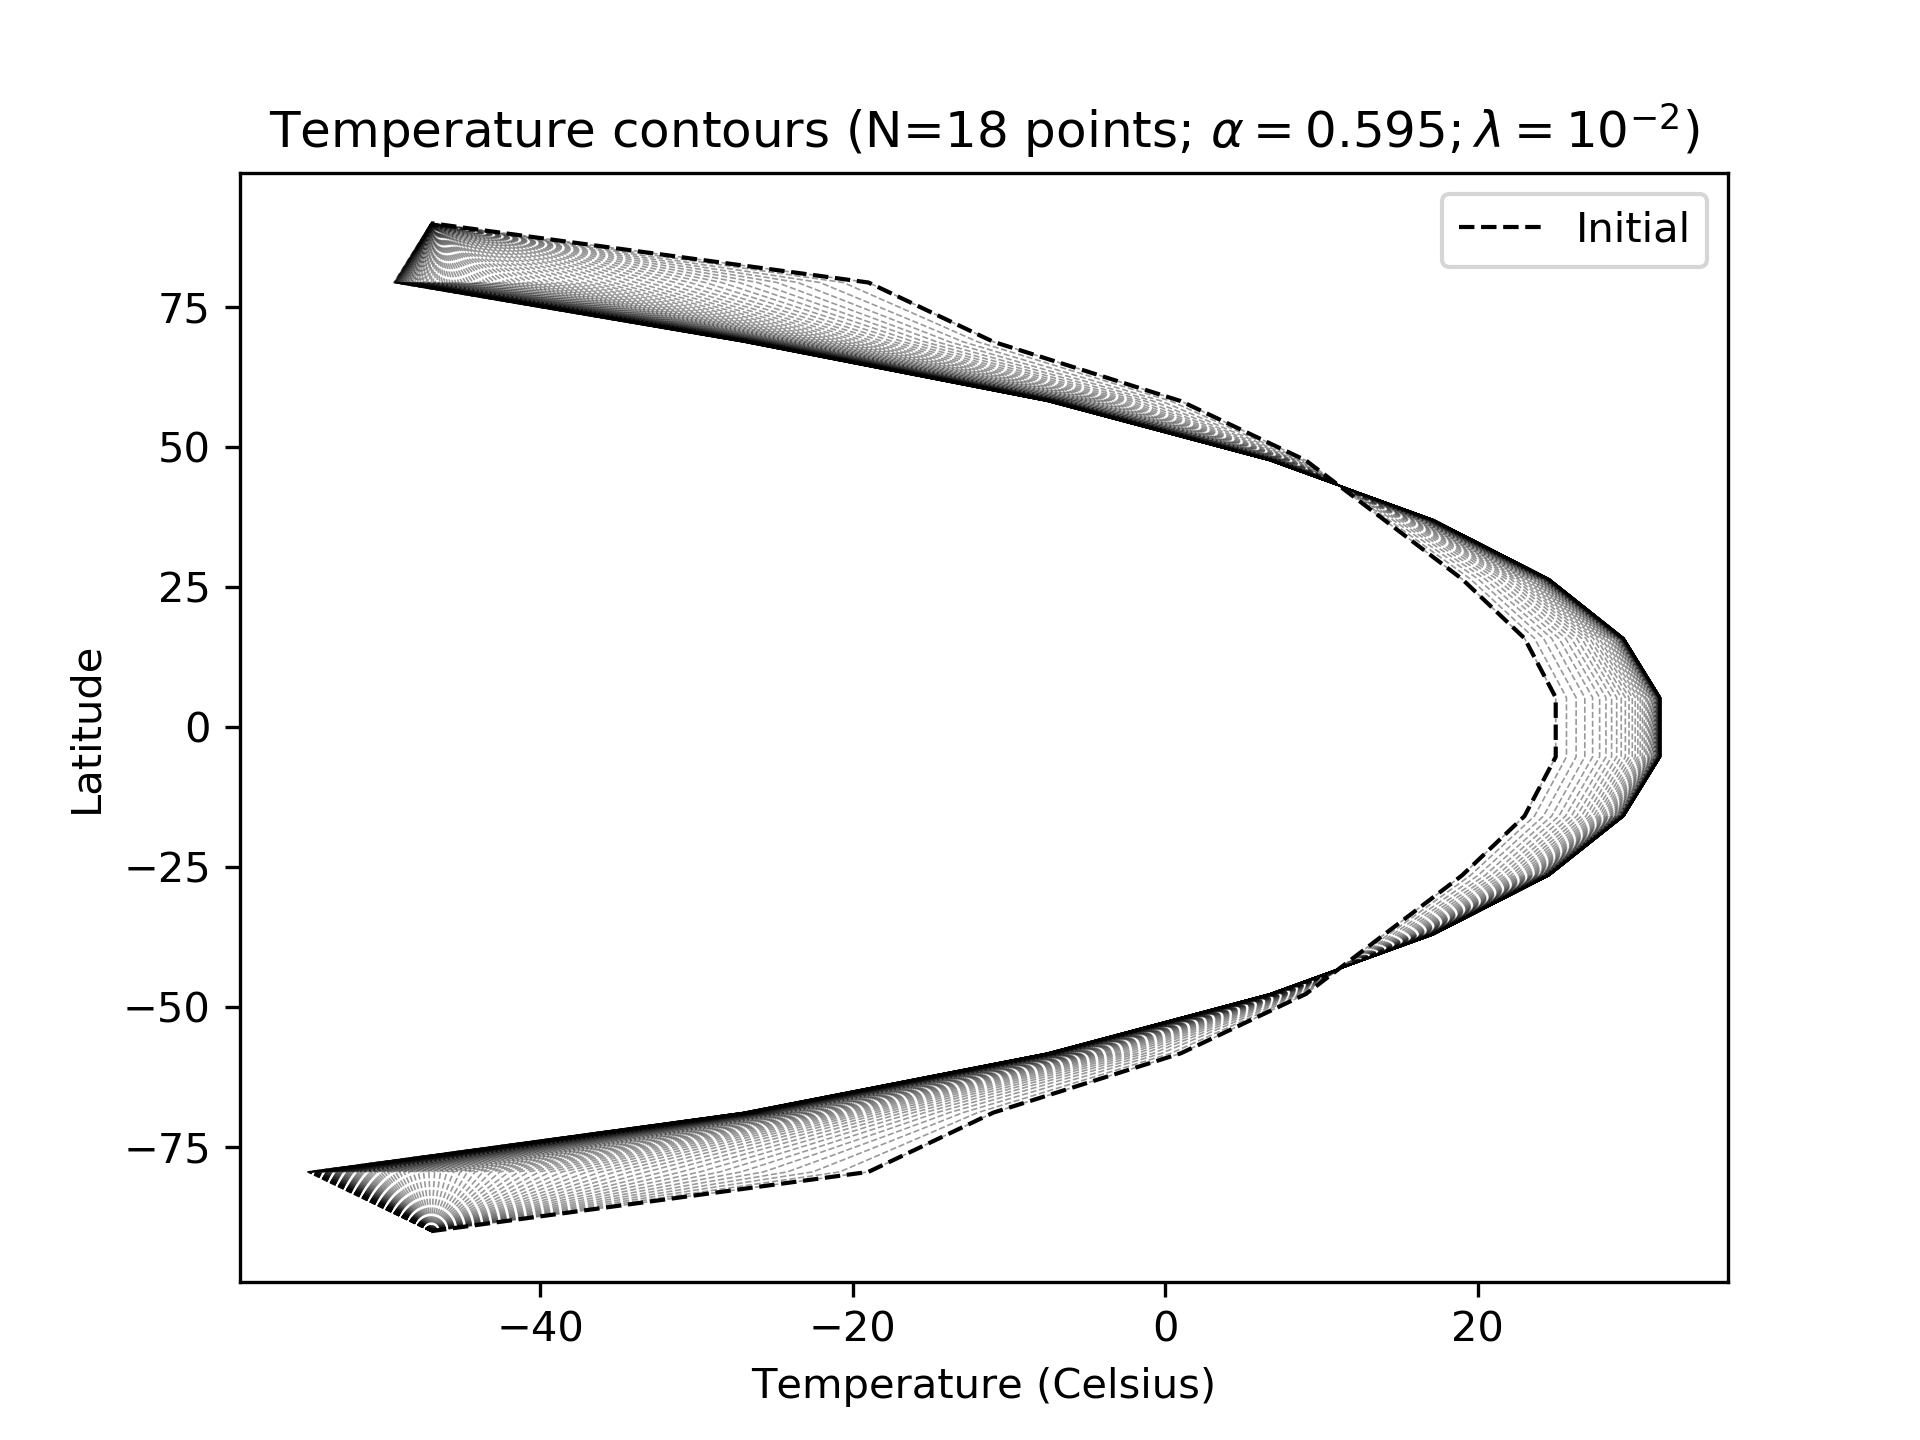
\includegraphics[scale=0.7]{tcont_q3.png} 
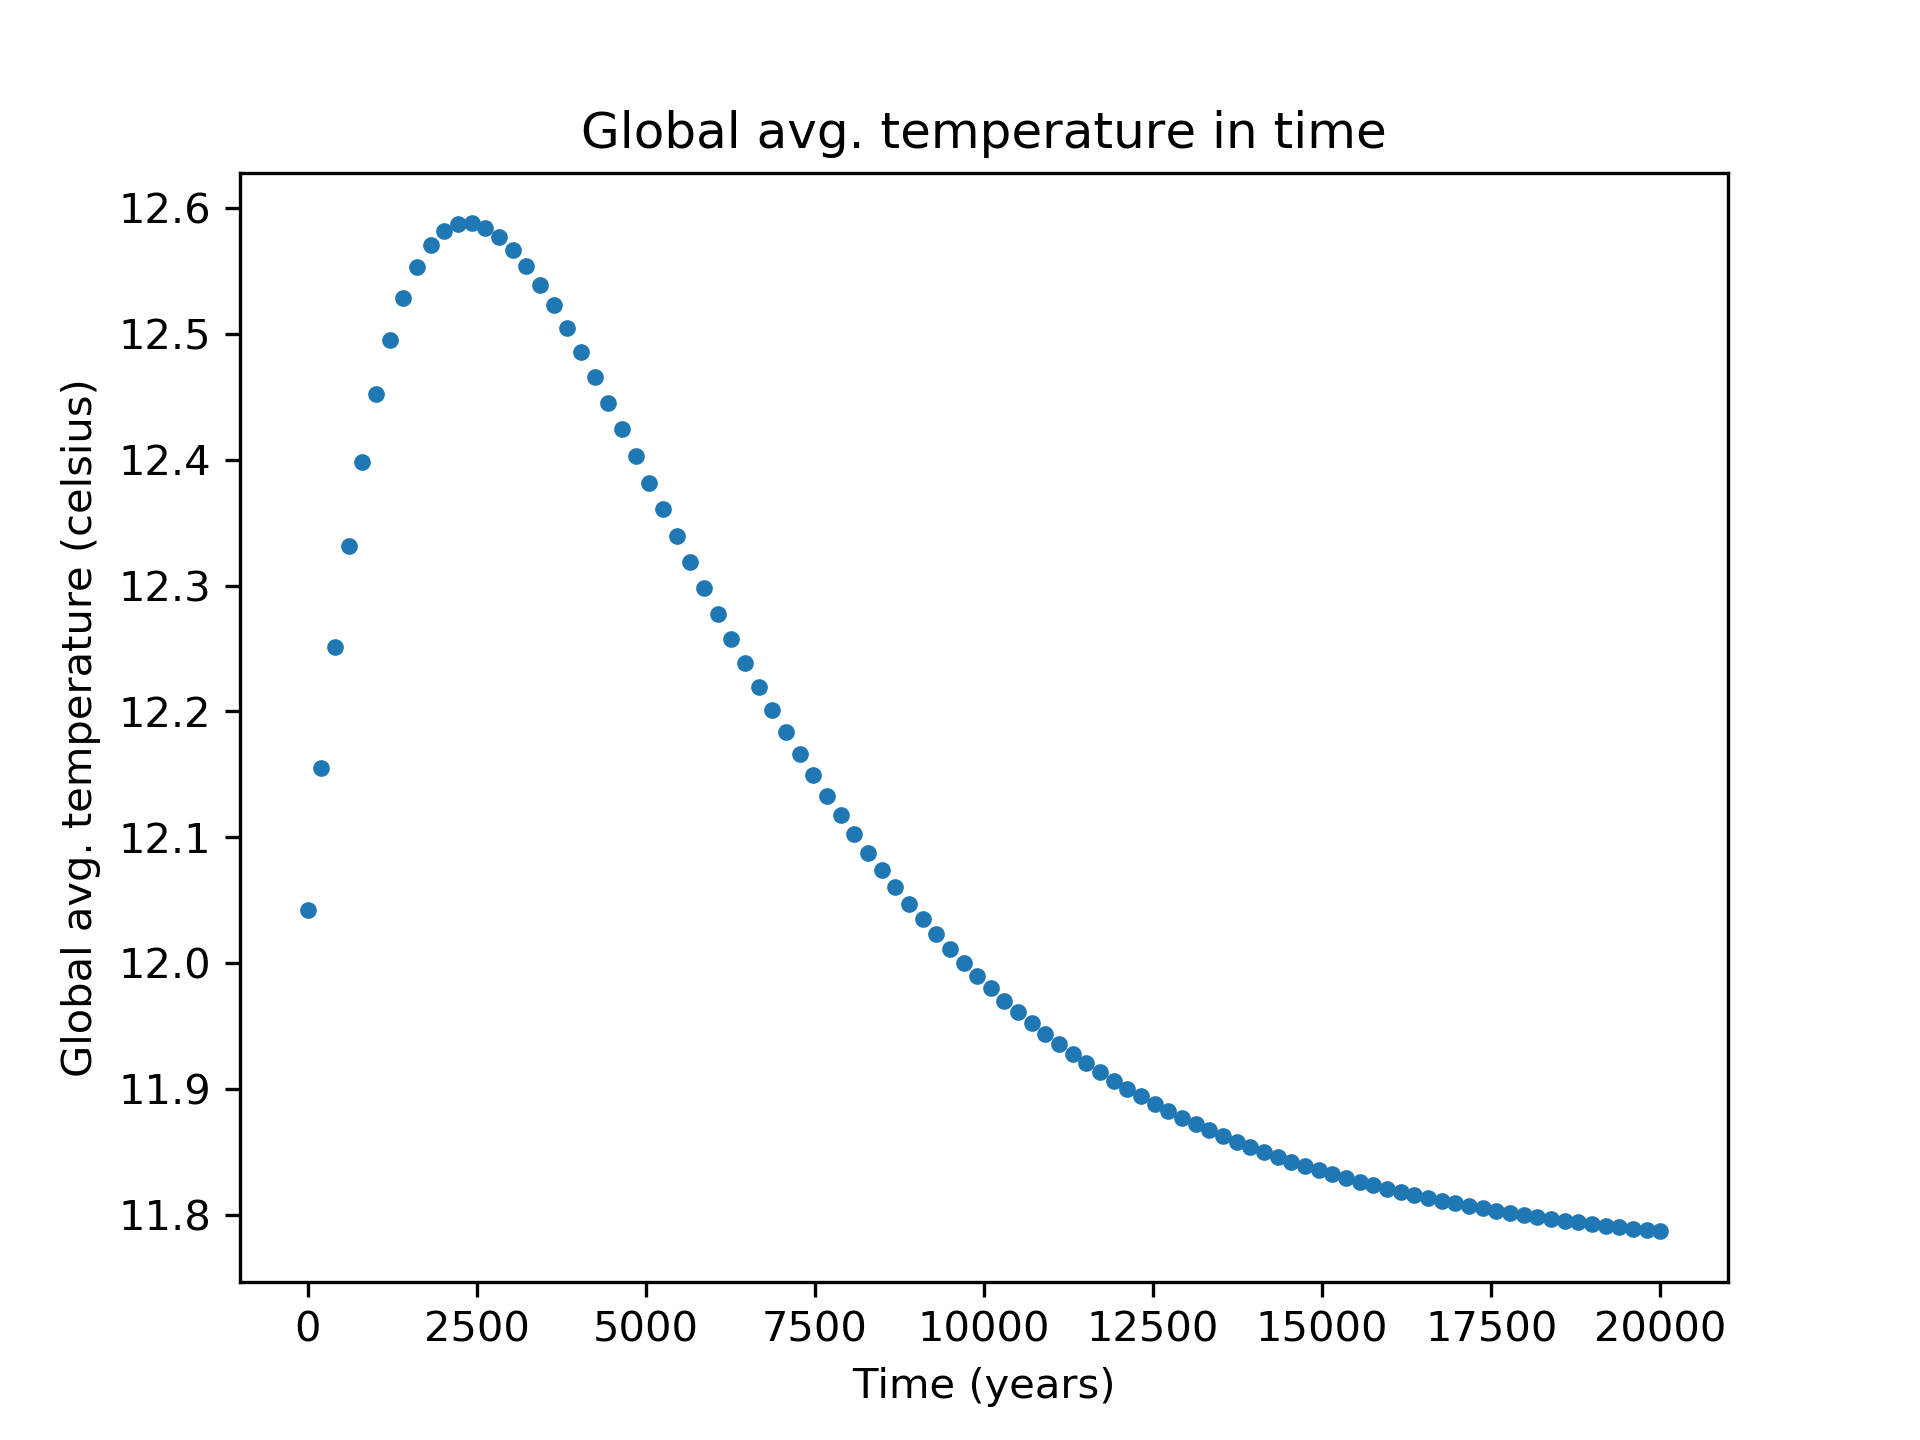
\includegraphics[scale=0.7]{tavg_q3.png}
\caption{Temperature isolines and global avg. temperature for optimum diffusivity and emissivity.}
\end{figure}

\section*{Question 3}
The optimum values of emissivity and diffusivity are: $\epsilon = 0.59,  \lambda = 0.01$. I chose these values because they best match the zonal temperature distribution given in the previous question and the loss of heat over time is minimal (Fig. 6).

\section*{Question 4}
\begin{figure}
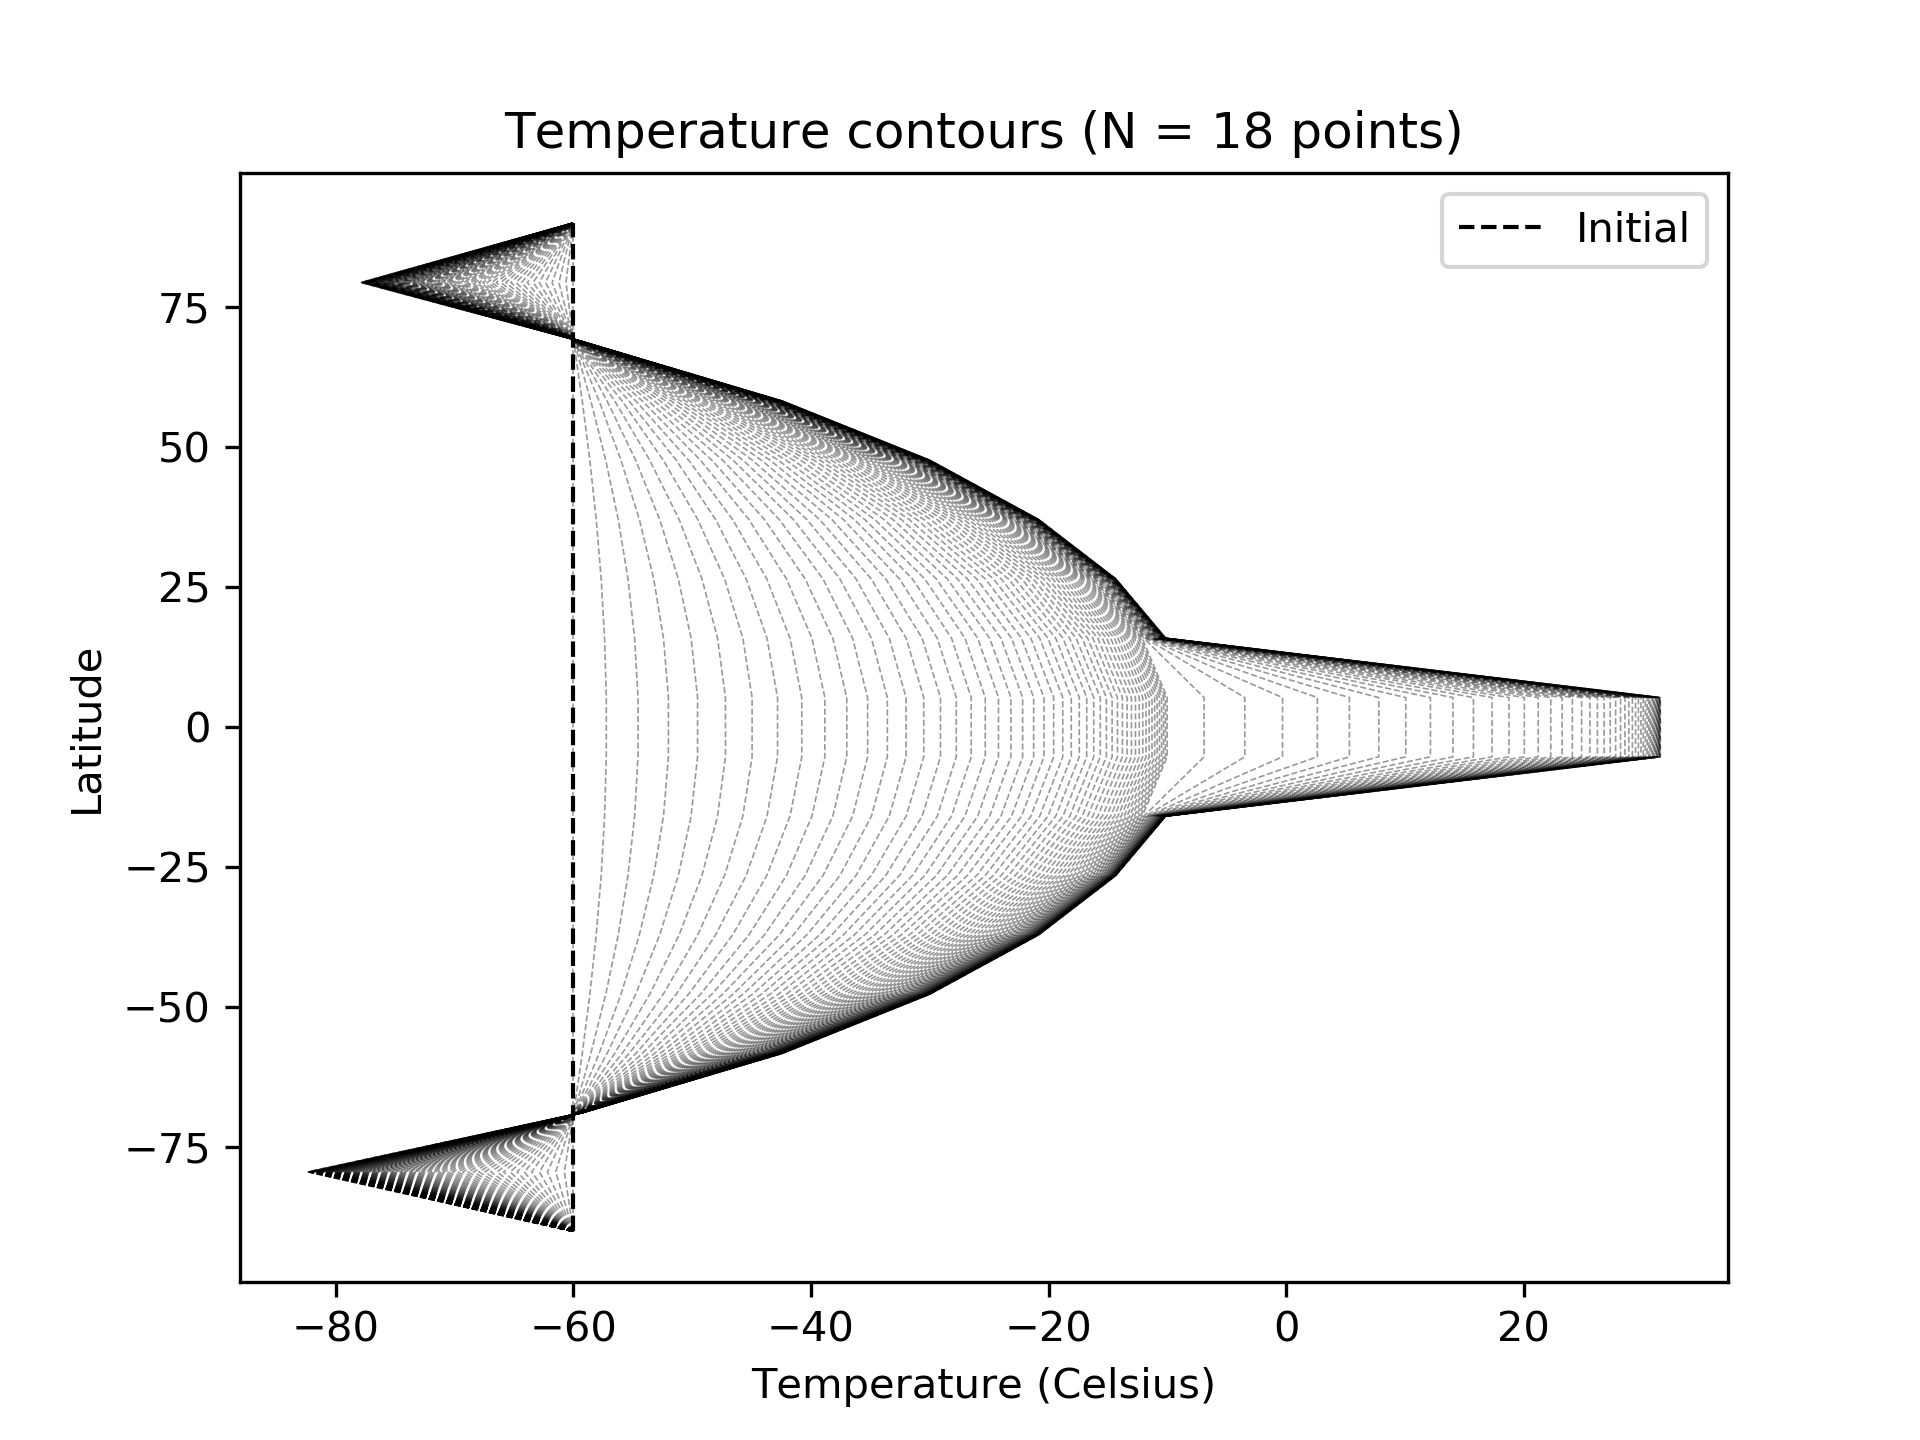
\includegraphics[scale=0.7]{tcont_q4.png} 
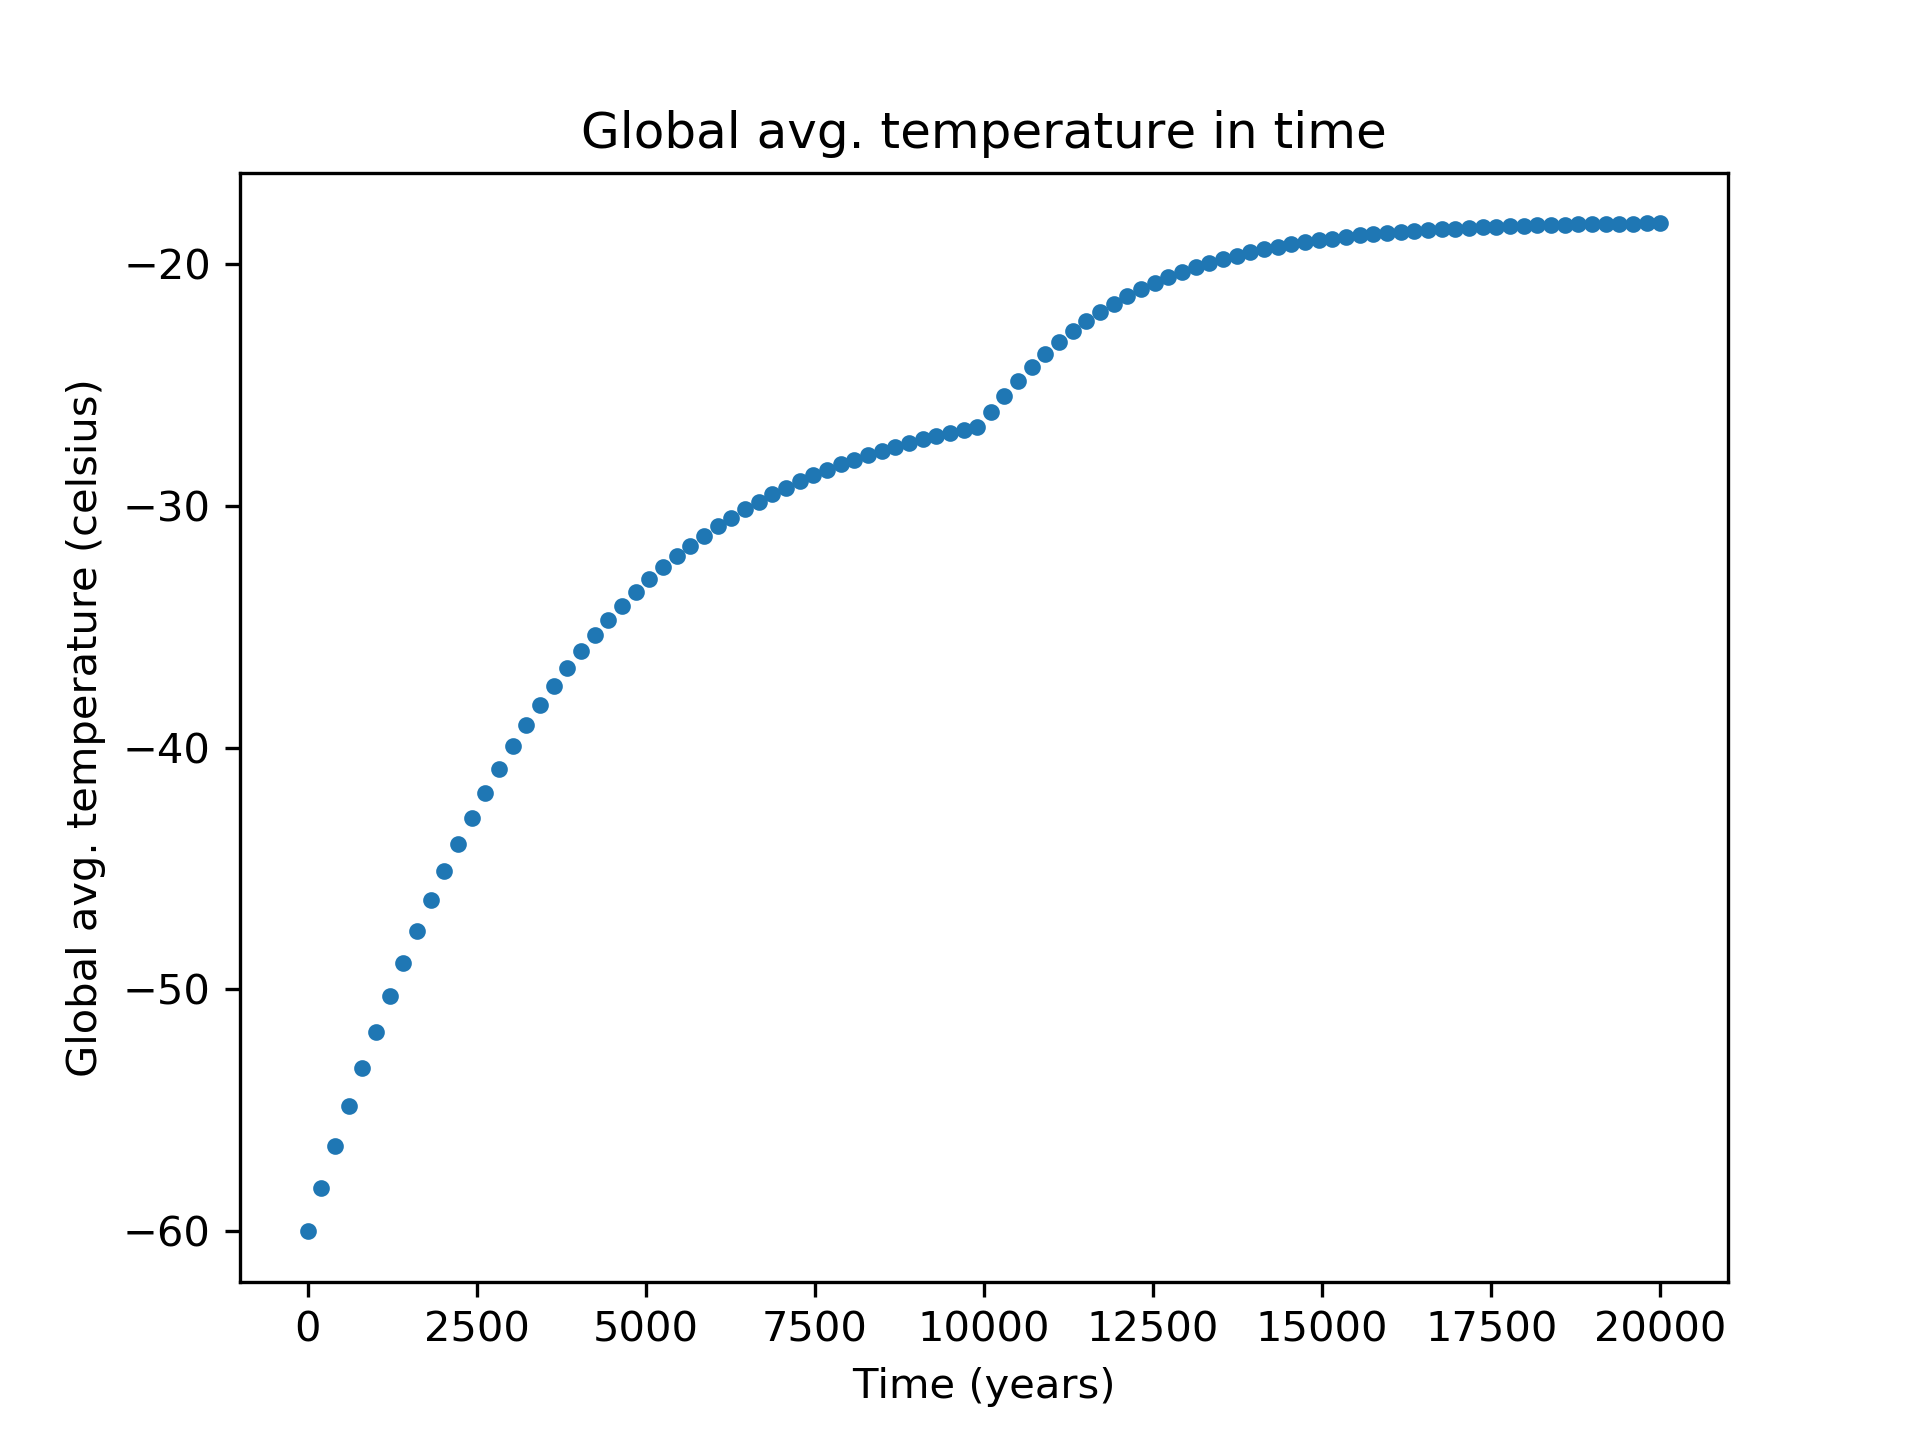
\includegraphics[scale=0.7]{tavg_q4.png}
\caption{Temperature isolines and global avg. temperature for -60 degrees celsius initial temperature.}
\end{figure}

\begin{figure}
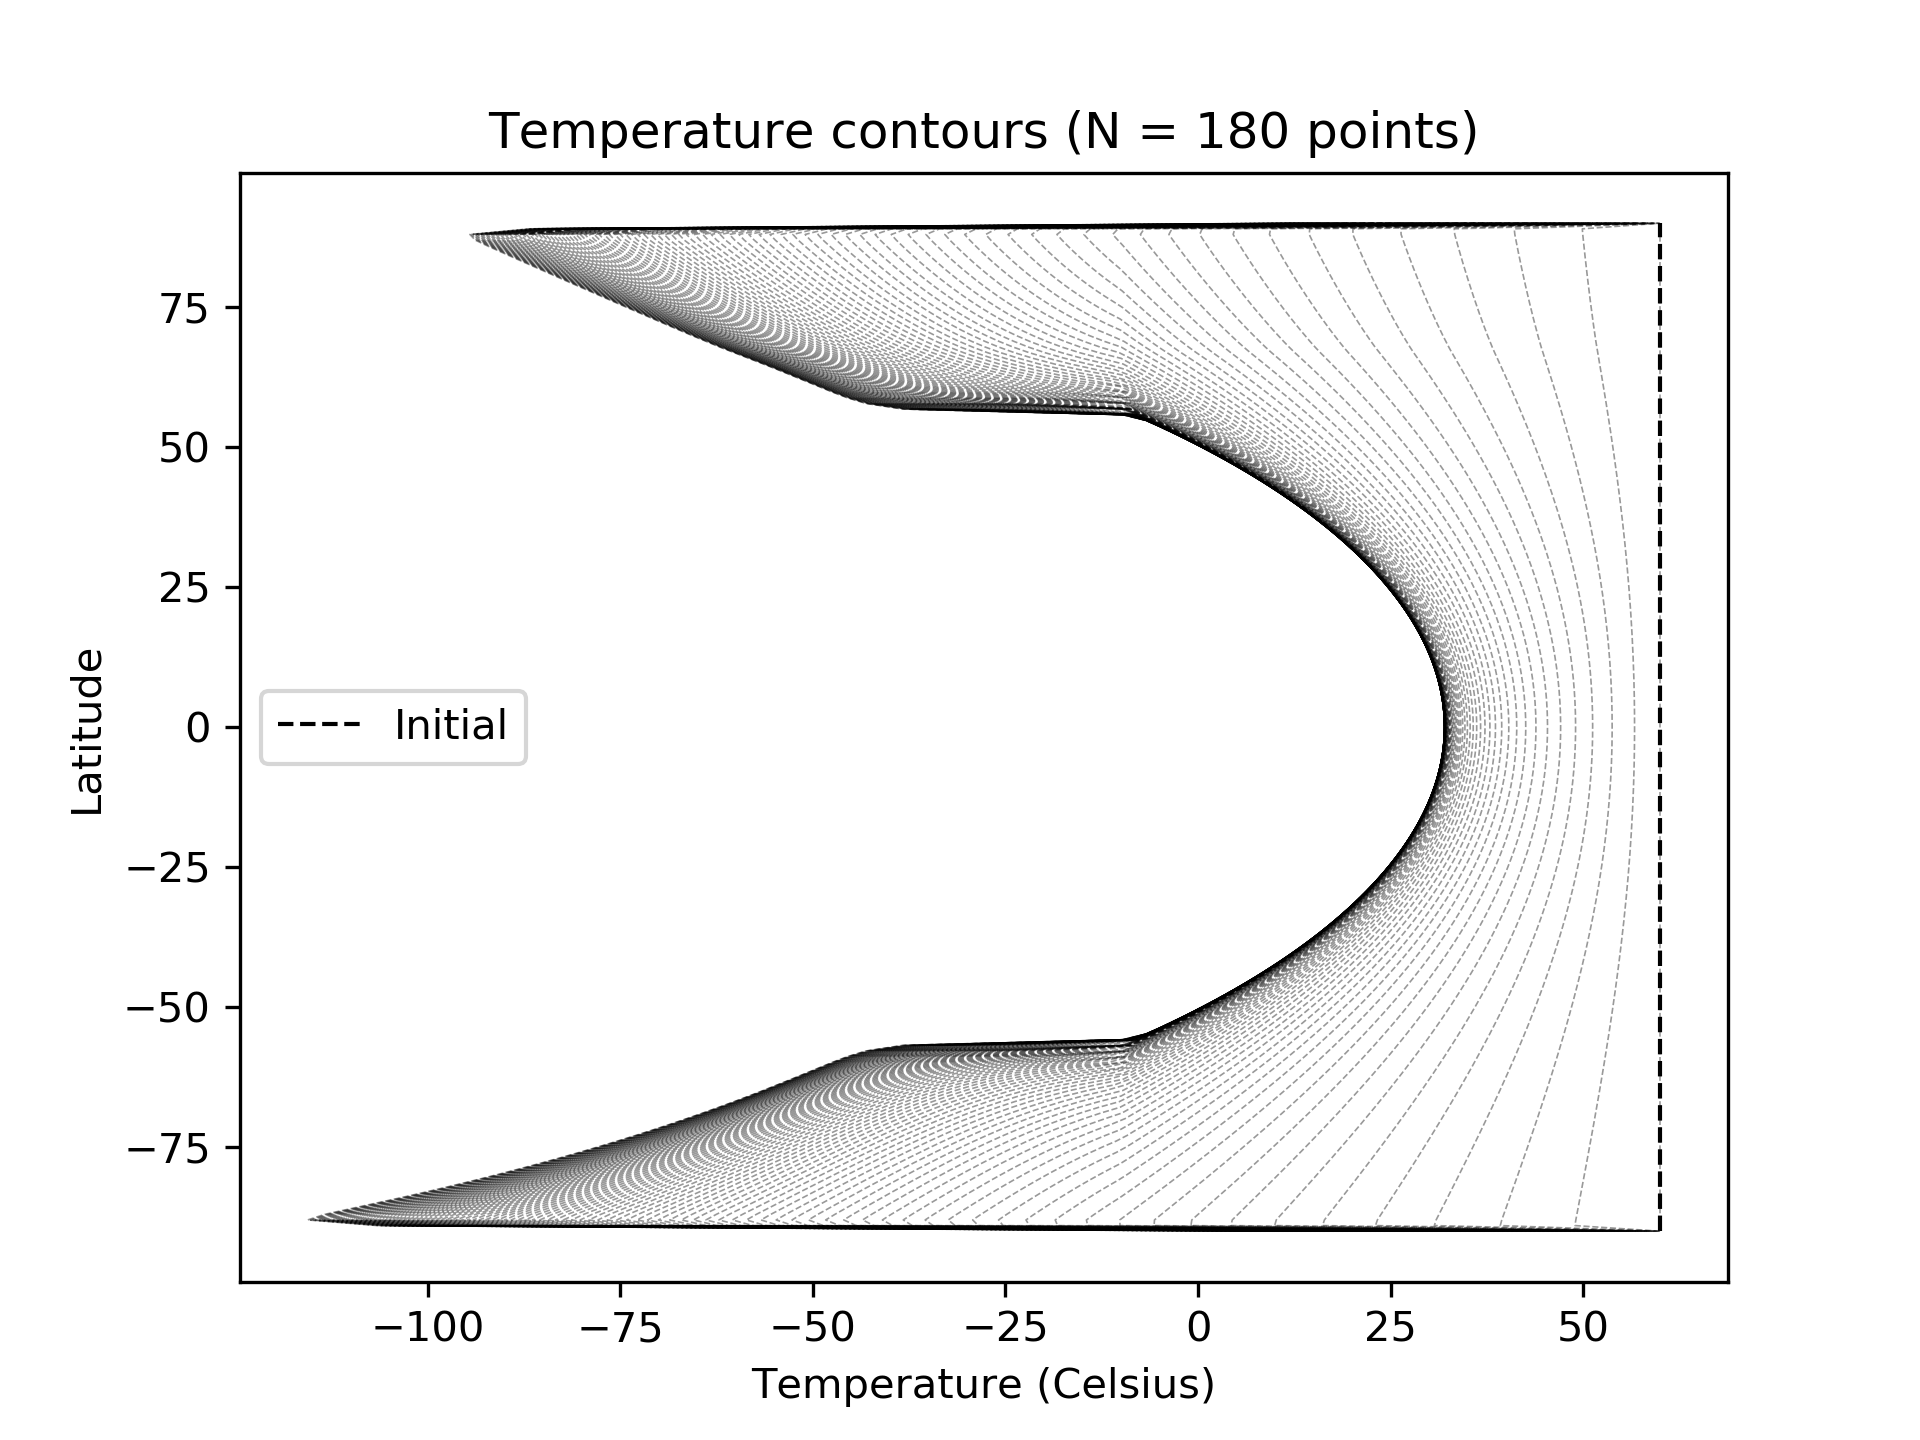
\includegraphics[scale=0.7]{tcont_q4c.png} 
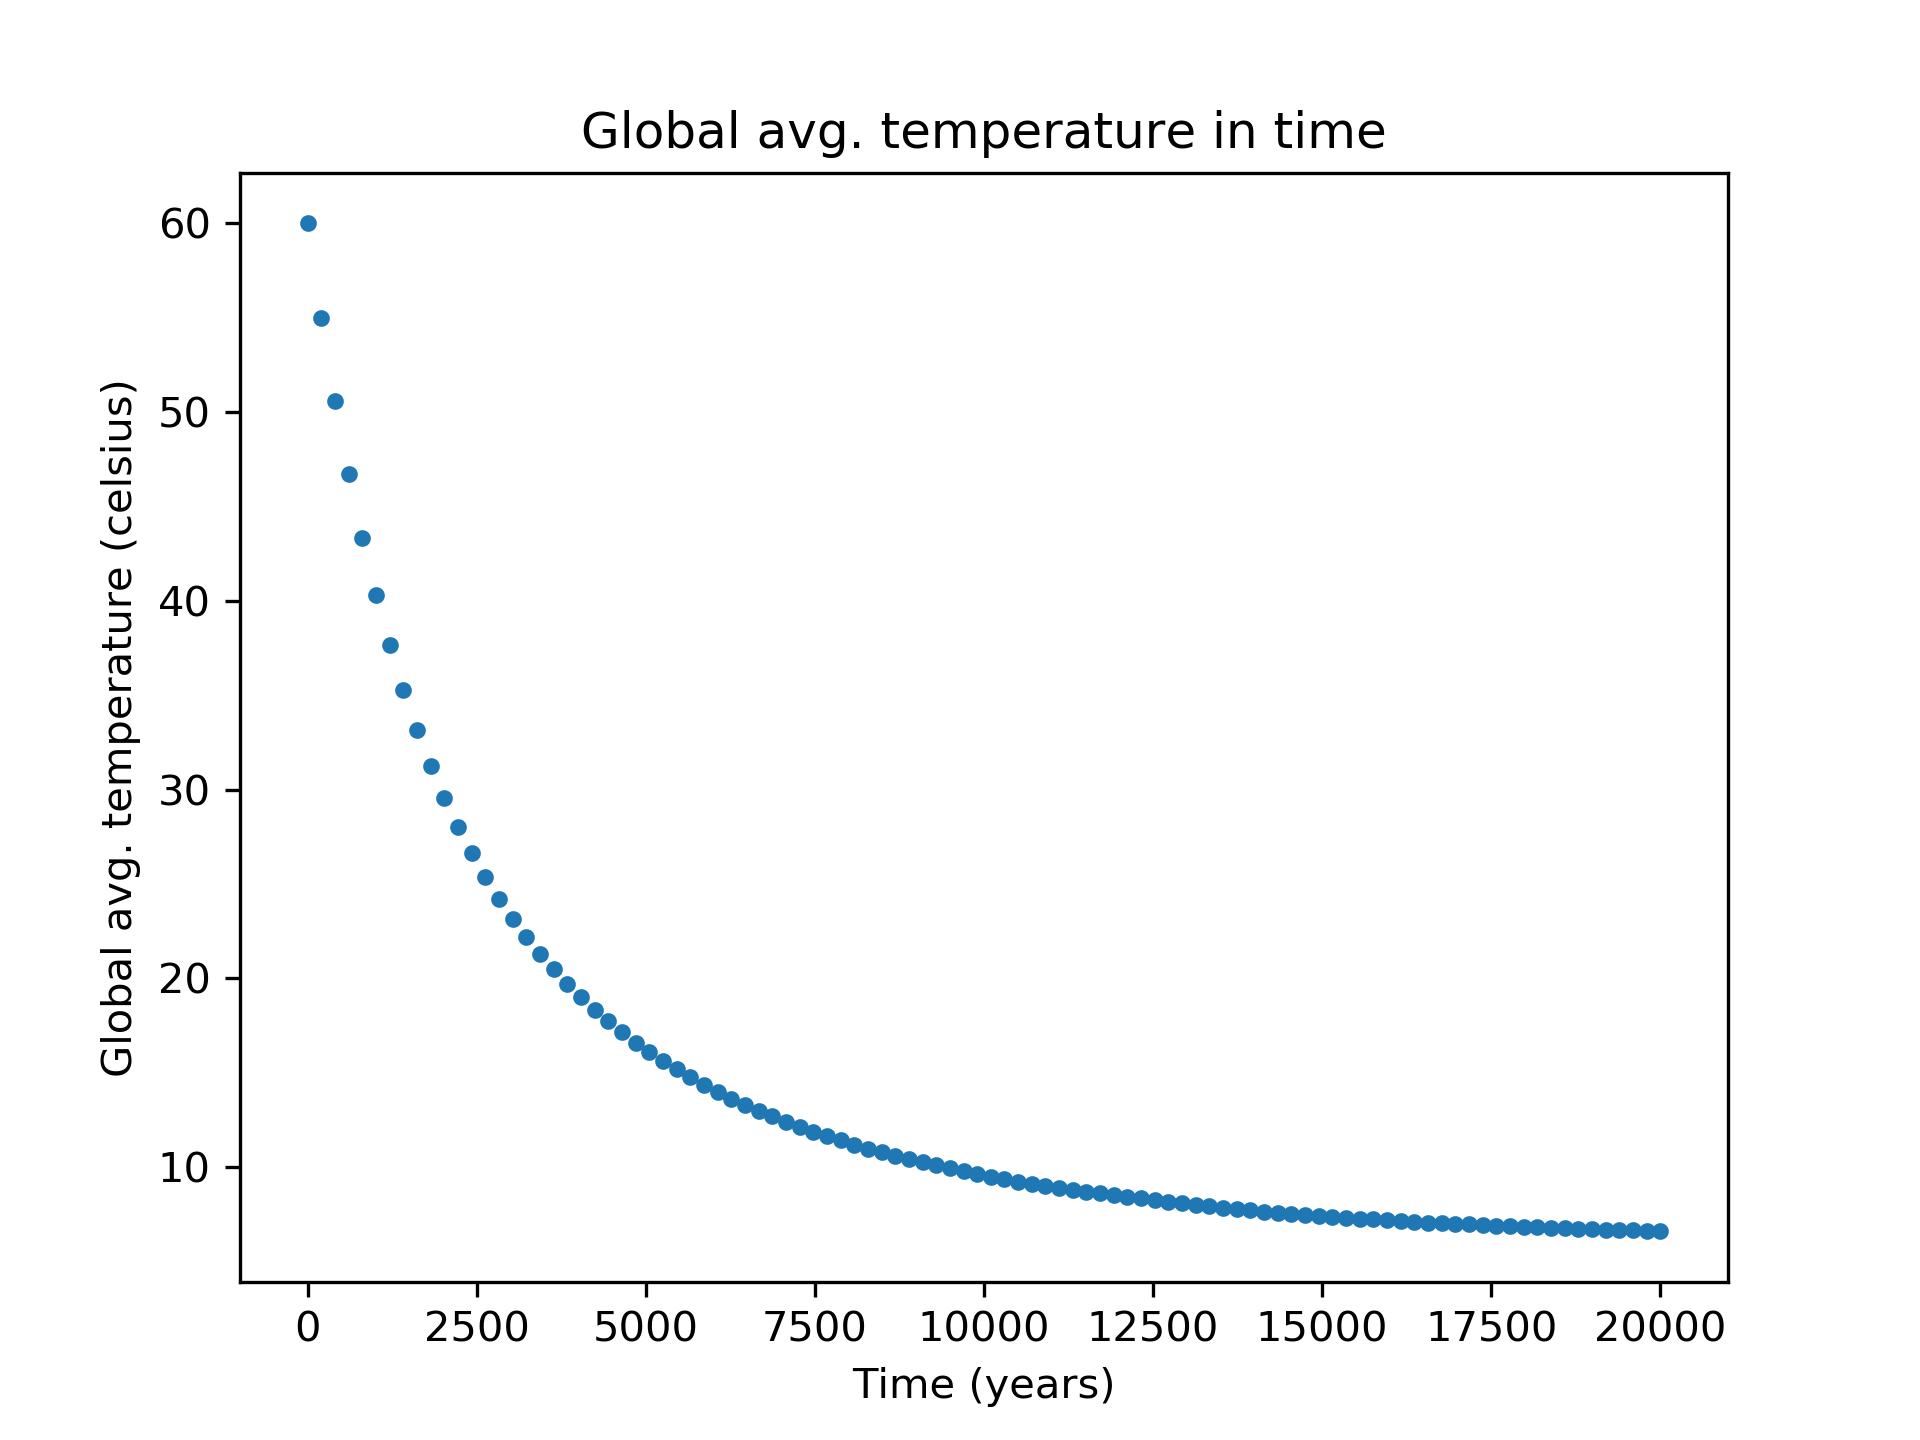
\includegraphics[scale=0.7]{tavg_q4c.png}
\caption{Temperature isolines and global avg. temperature for +60 degrees celsius initial condition.}
\end{figure}

\begin{figure}
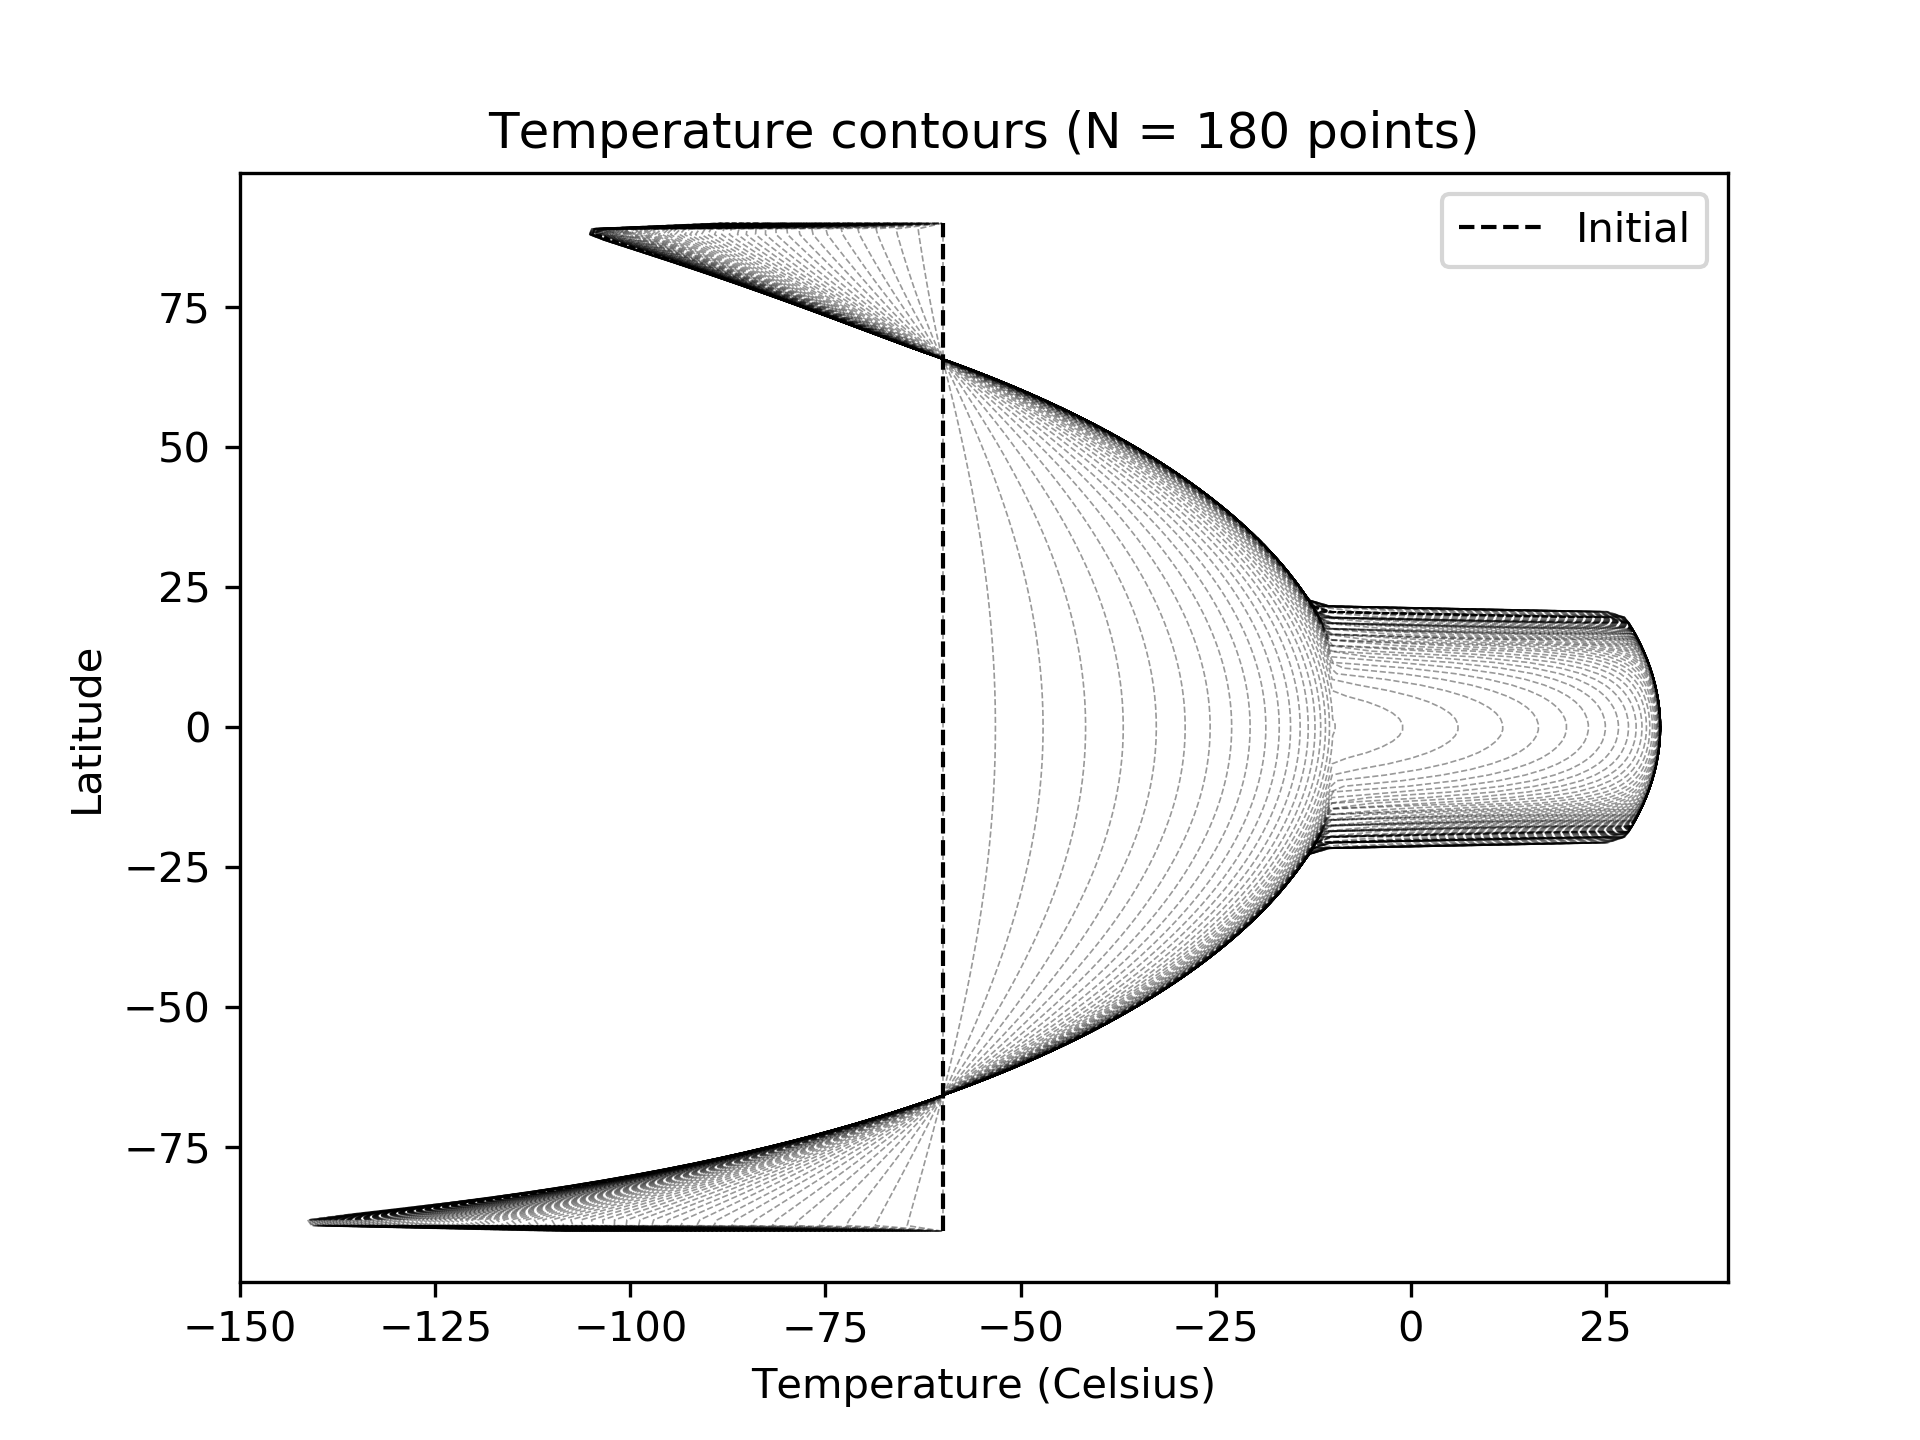
\includegraphics[scale=0.7]{tcont_q4b.png} 
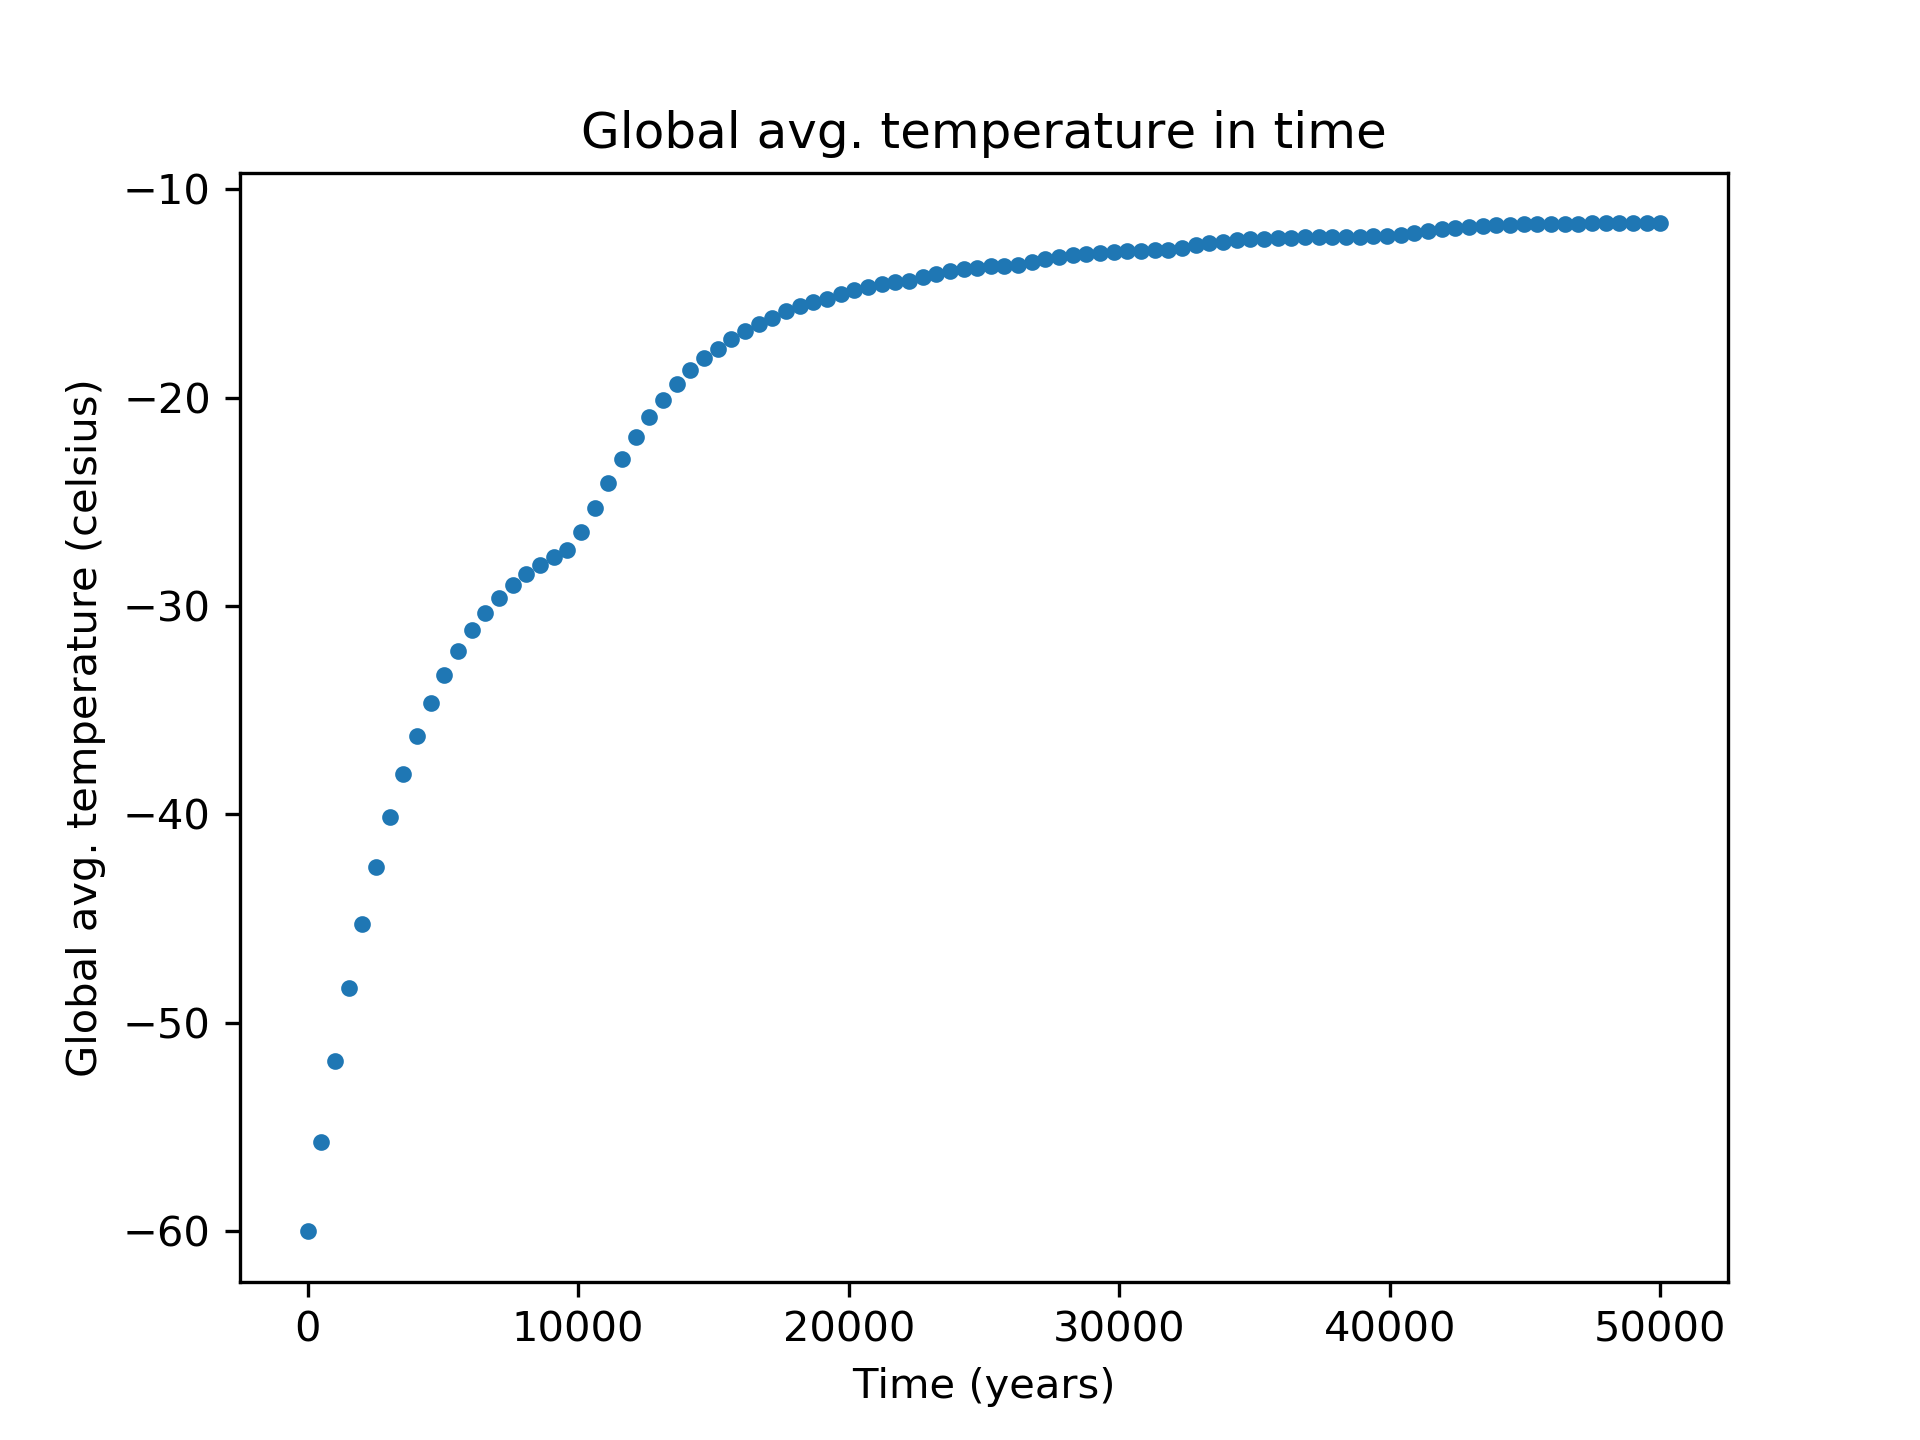
\includegraphics[scale=0.7]{tavg_q4b.png}
\caption{Temperature isolines and global avg. temperature with higher resolution.}
\end{figure}

We see that for the initial temperature of -60 degrees celsius, there is a sharp rise in the average temperature. As the part of the planet reachees outside the ice zone, we see a sharp discontinuity due to the change in albedo, and the temperature near that region (equator) rises much higher. For an initial temperature of +60 degrees celsius, we see a decrease in the temperature isoline. We again observe discontinuity when the temperature goes below the freezing limit of -10 degree celsius (Fig. 7, 8, 9). We see that for a higher resolution (Fig. 9), the curves get smoother although there is no qualitative difference than the coarse resolution. But the earth's tilt is much better incorporated in the finer resolution simulation. 


\section*{Question 5}
We see the effect of a solar multiplier constant on the subsequent heating and cooling of the planet. Below (Fig. 10) I show the temperature isolines for multiple simulations with different solar constants and the initial temperature feedback incorporated. In figure 11, we see the solar multiplier against the ice fraction and the steady dtate globally averaged temperature. We see that there are two inflection points on the red graph, where the global average temperature has zero slope. At these points, there will be no change in the temperature distribution as the time increases. Therefore, we can say that there are atleast two equilibrium solutions that earth's climate can support, one of which is completely glacial.  
\begin{figure}
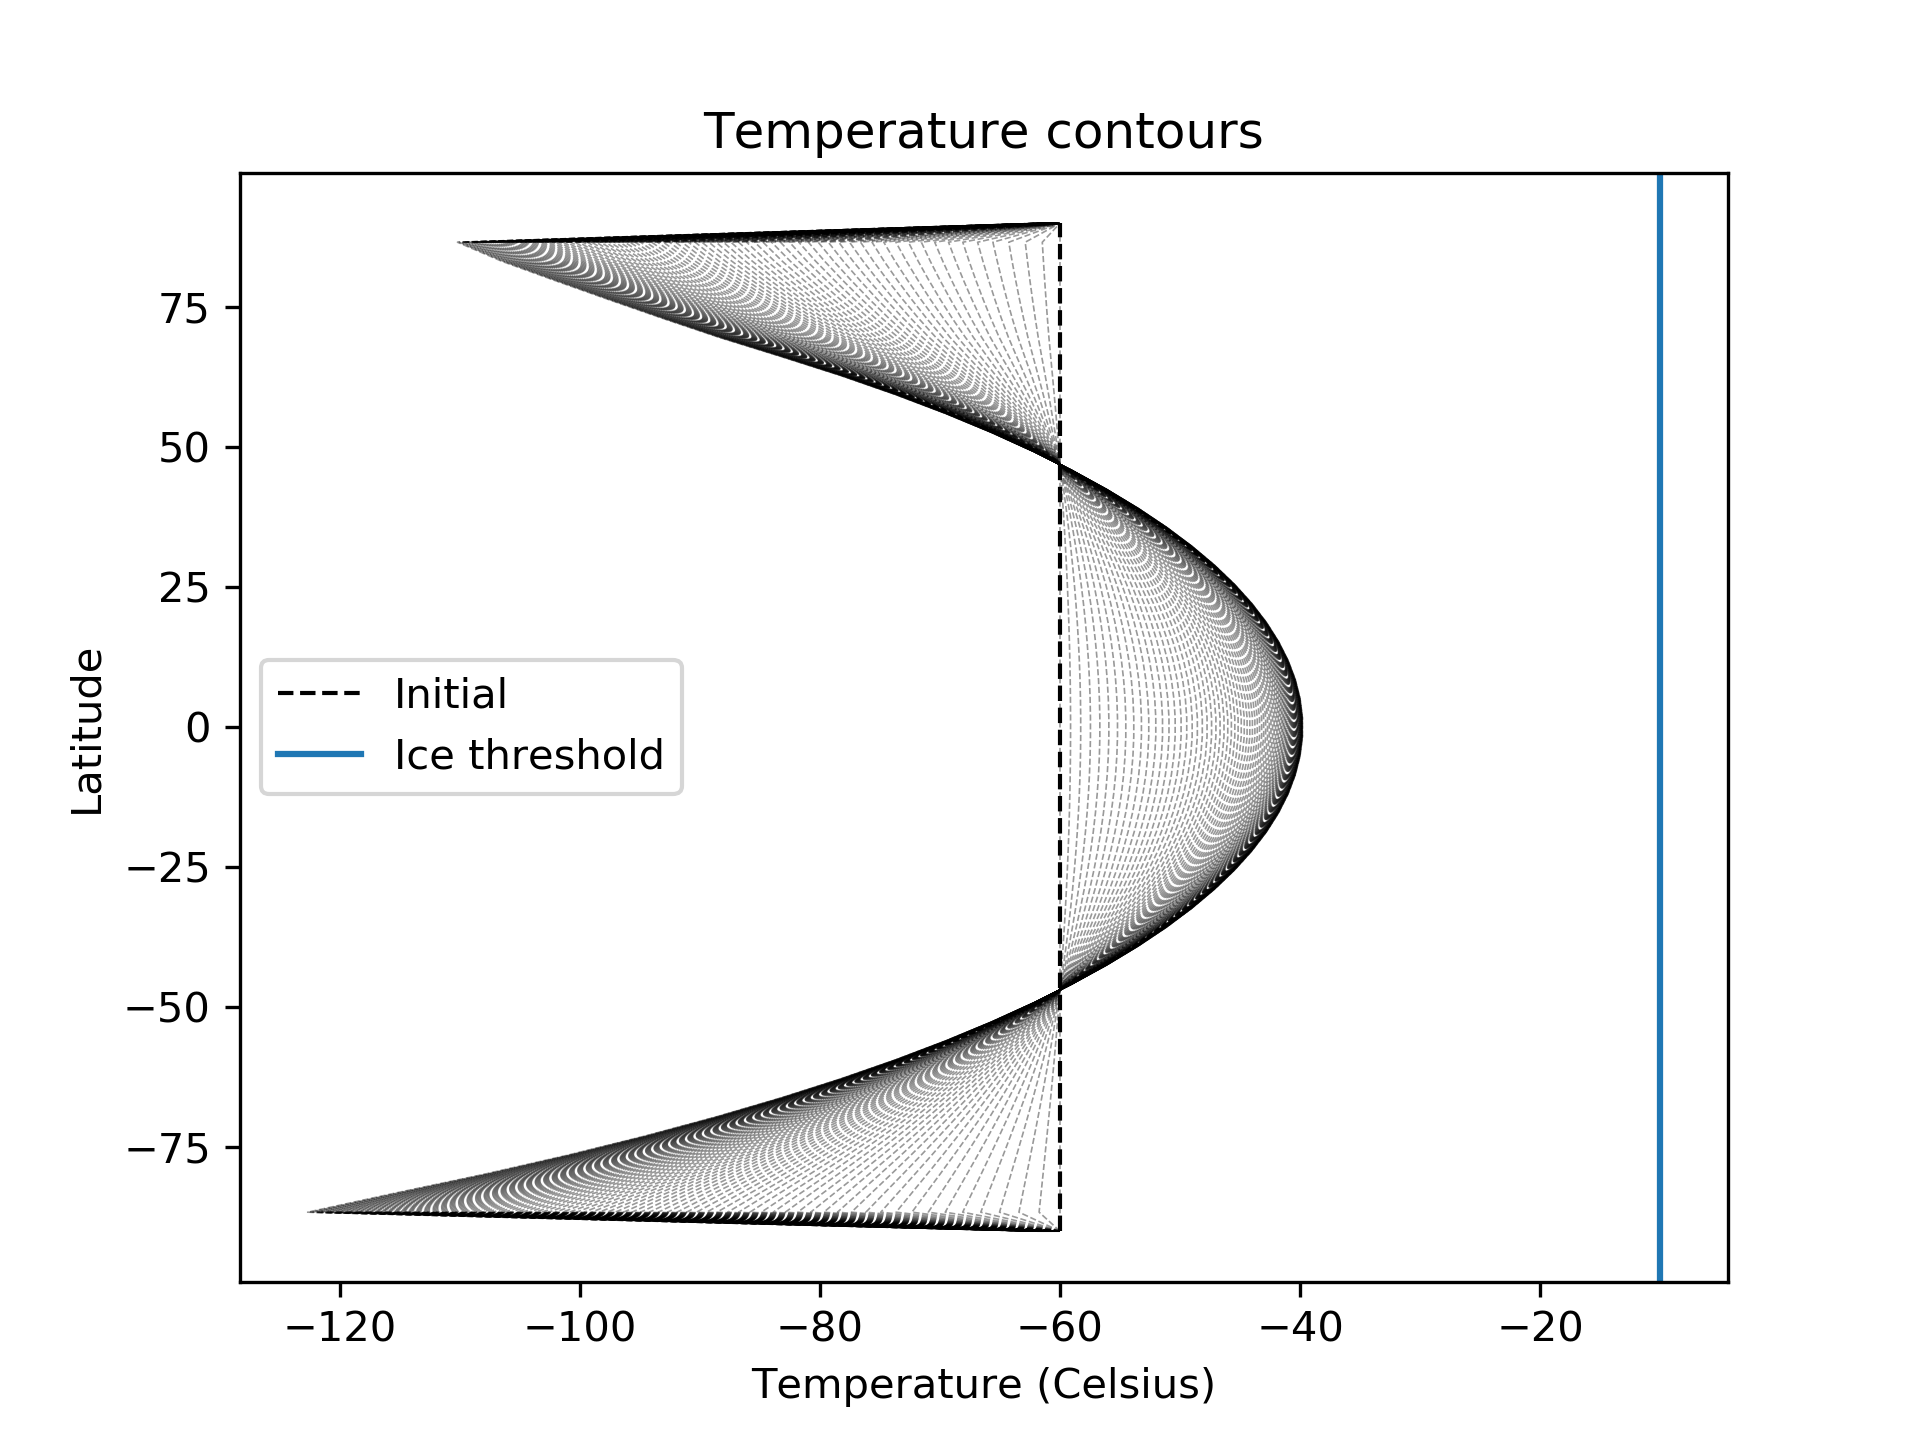
\includegraphics[scale=0.4]{tcont_50.png} 
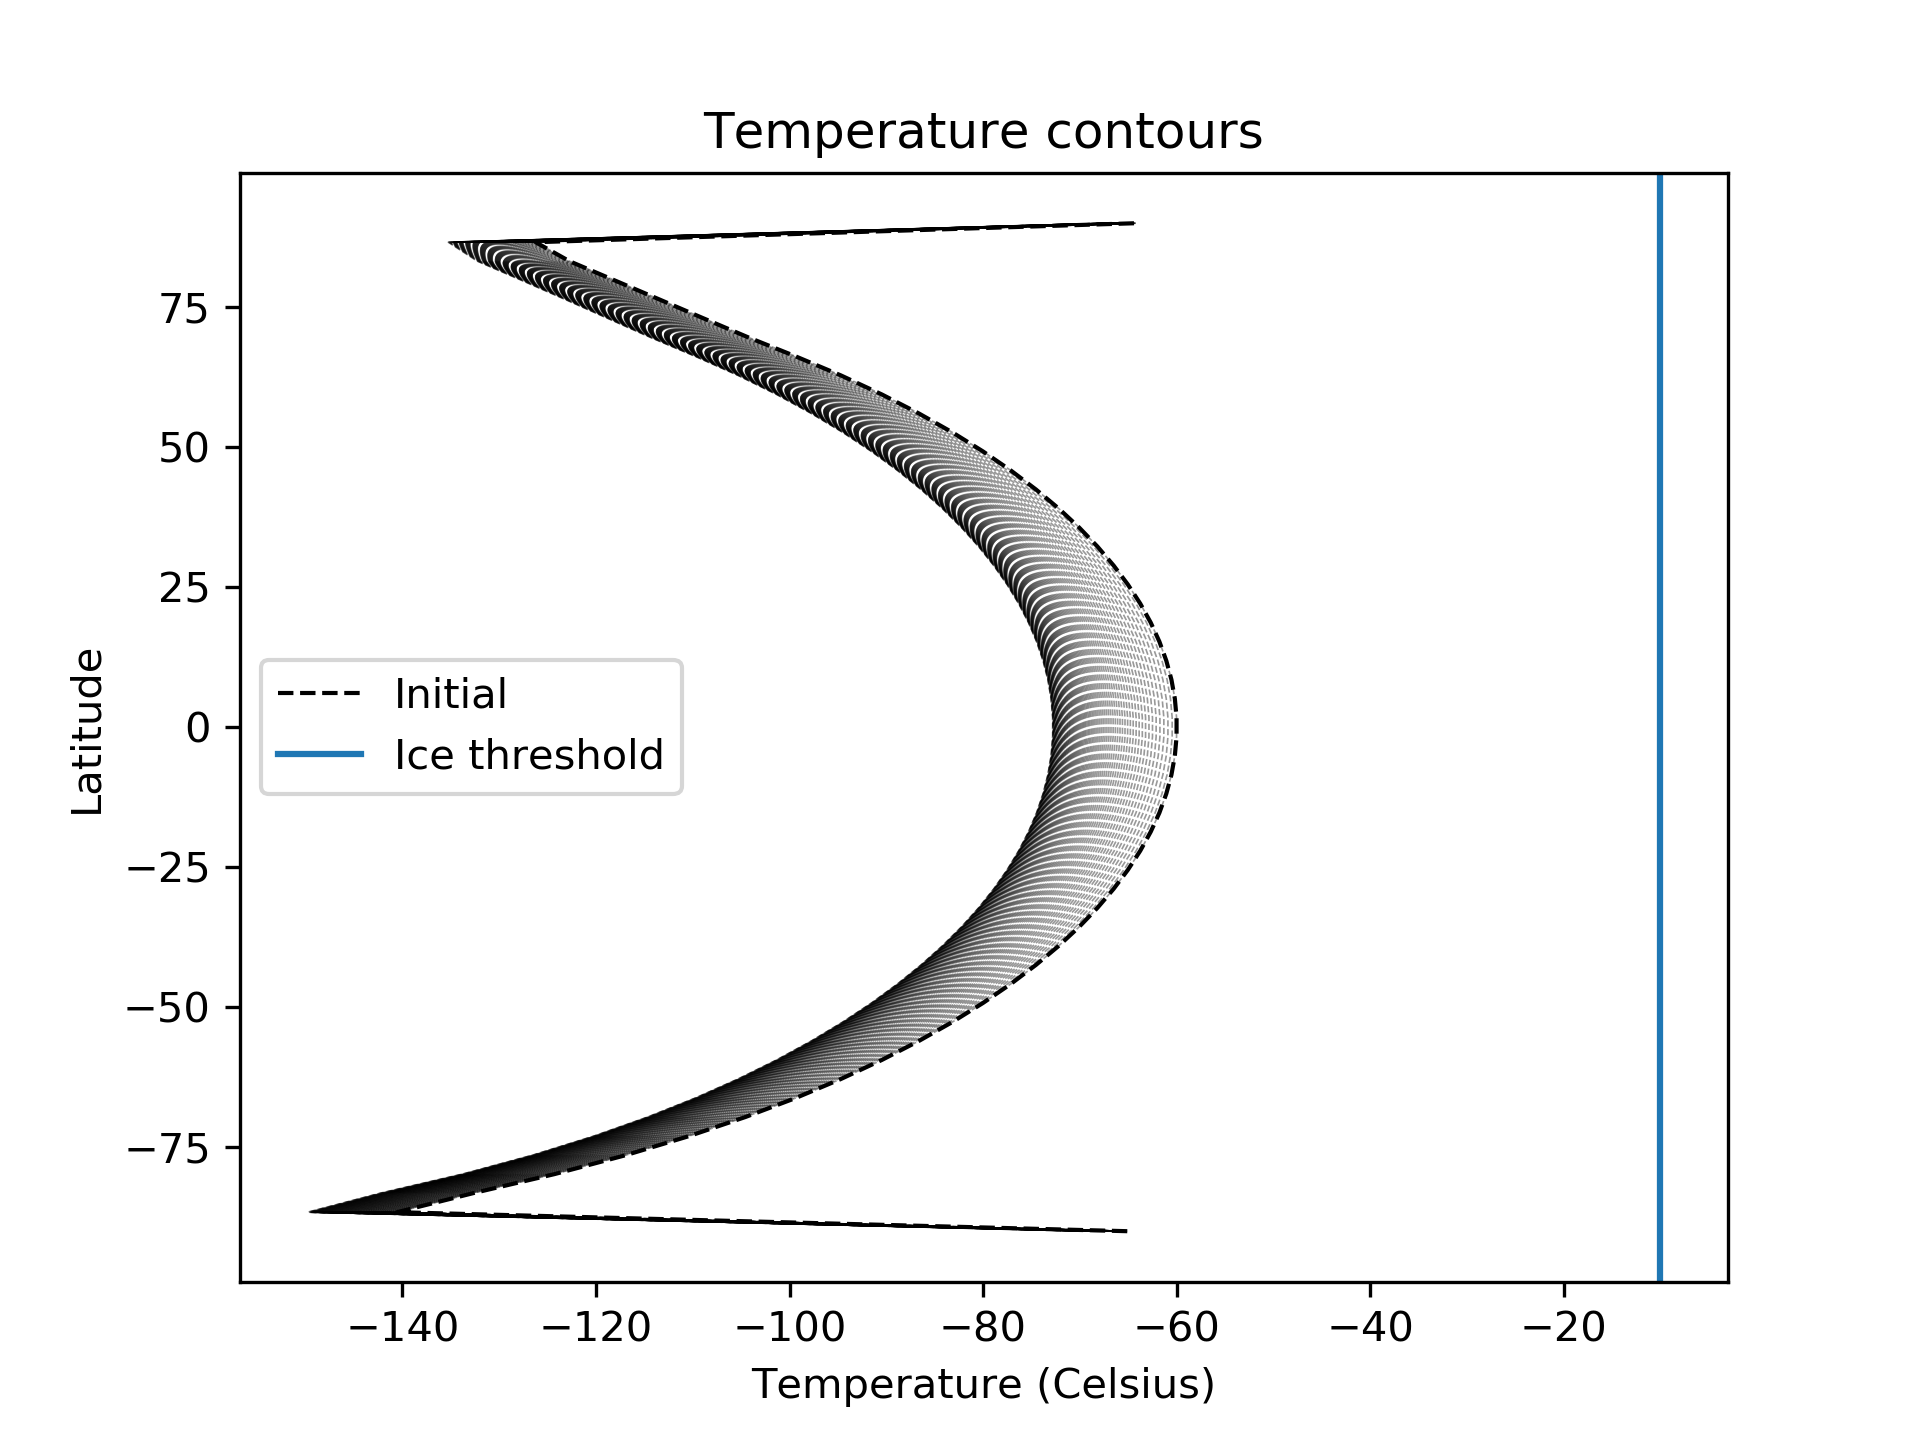
\includegraphics[scale=0.4]{tcont_52.png} 
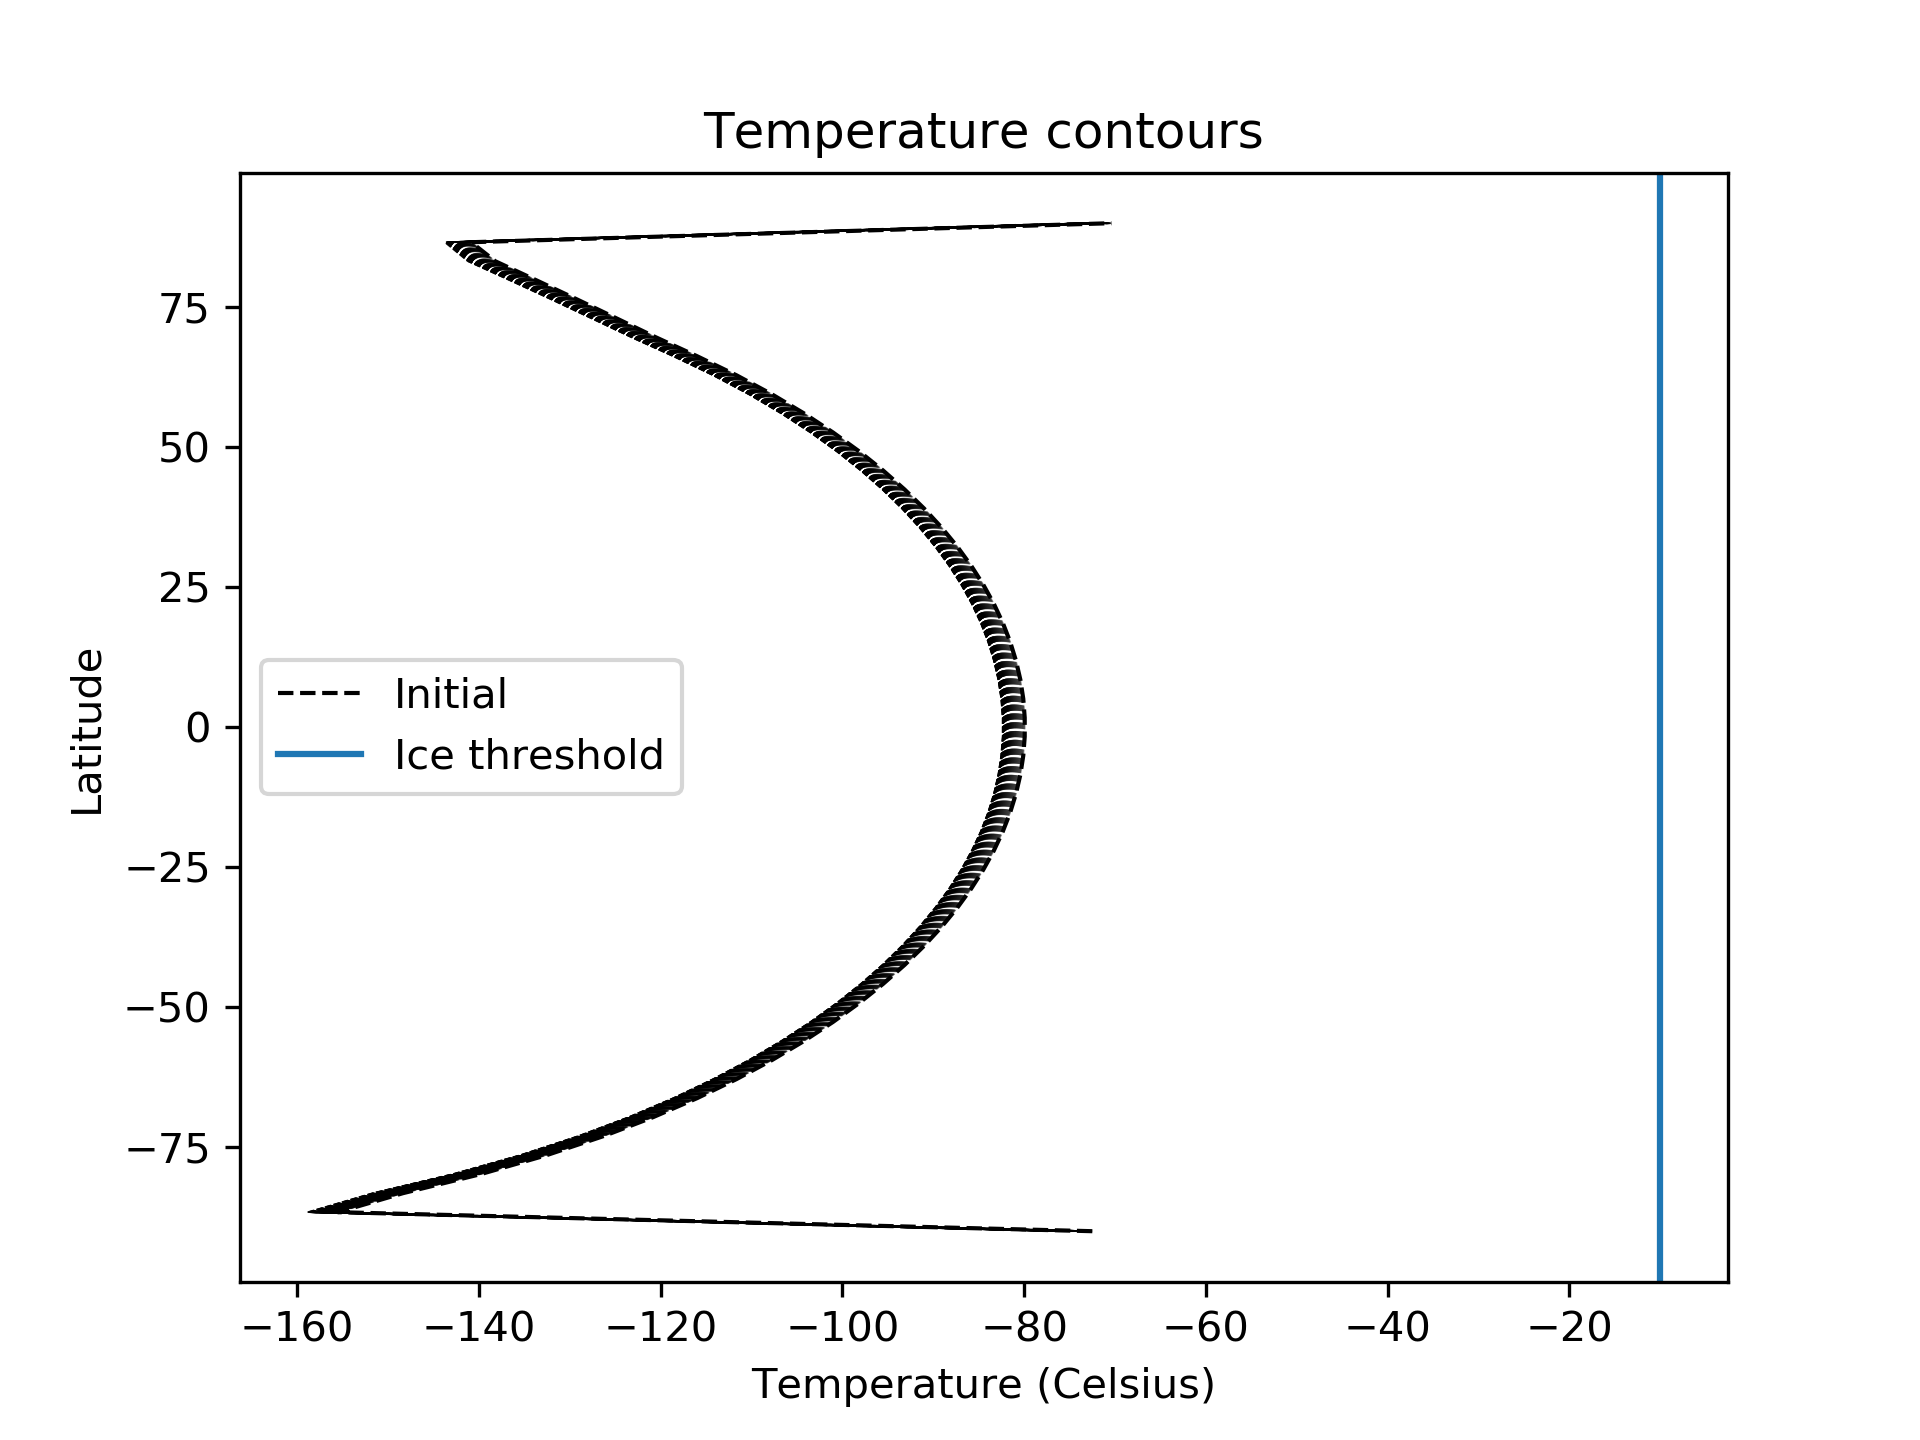
\includegraphics[scale=0.4]{tcont_54.png} 
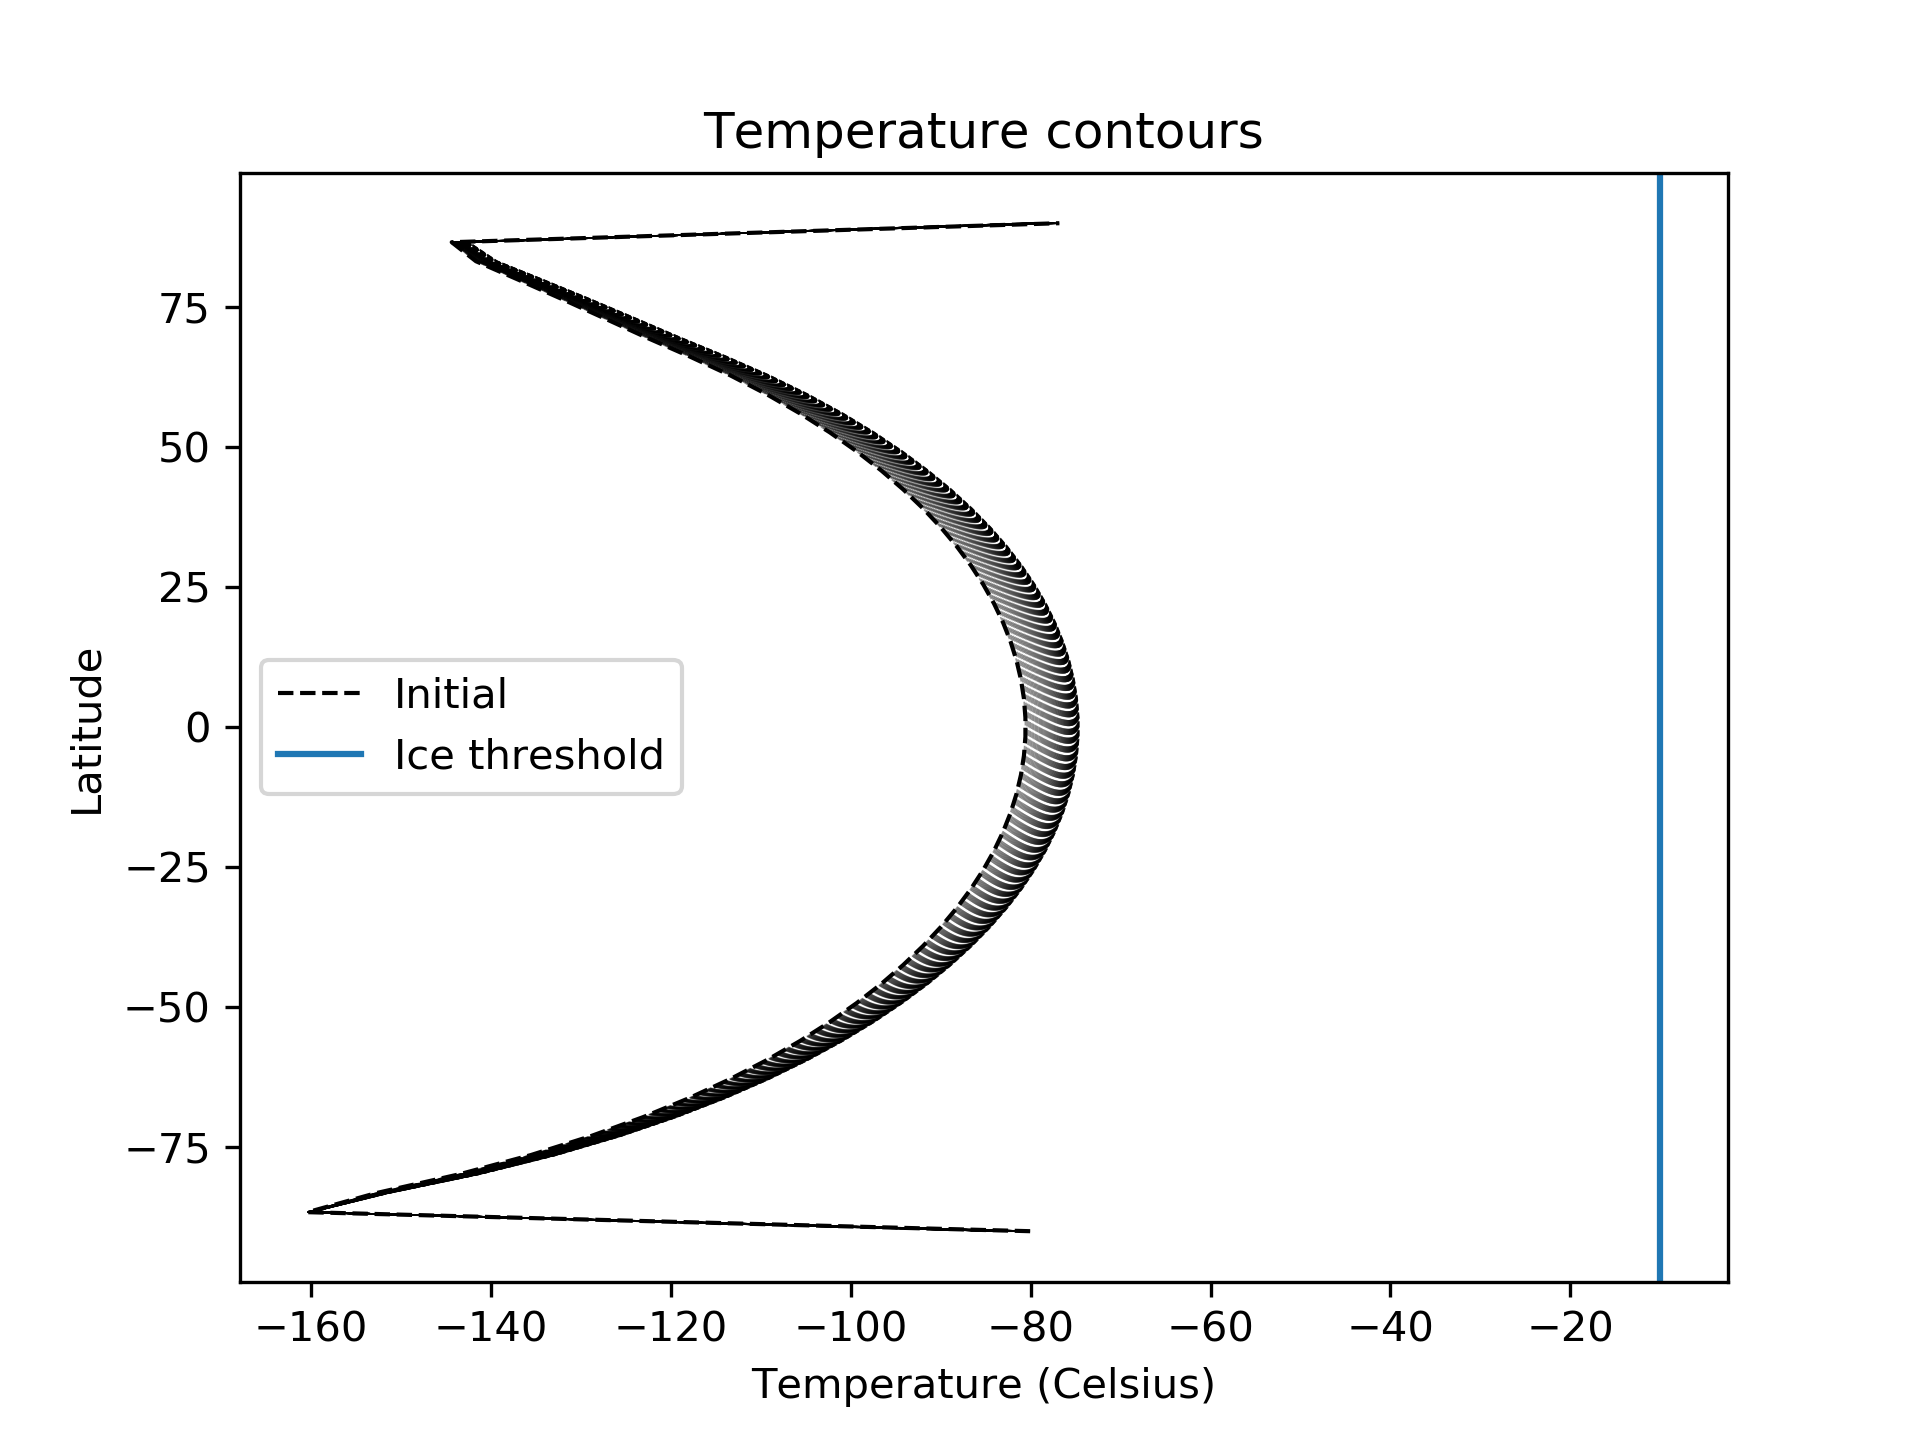
\includegraphics[scale=0.4]{tcont_56.png} 
\end{figure}
\begin{figure}
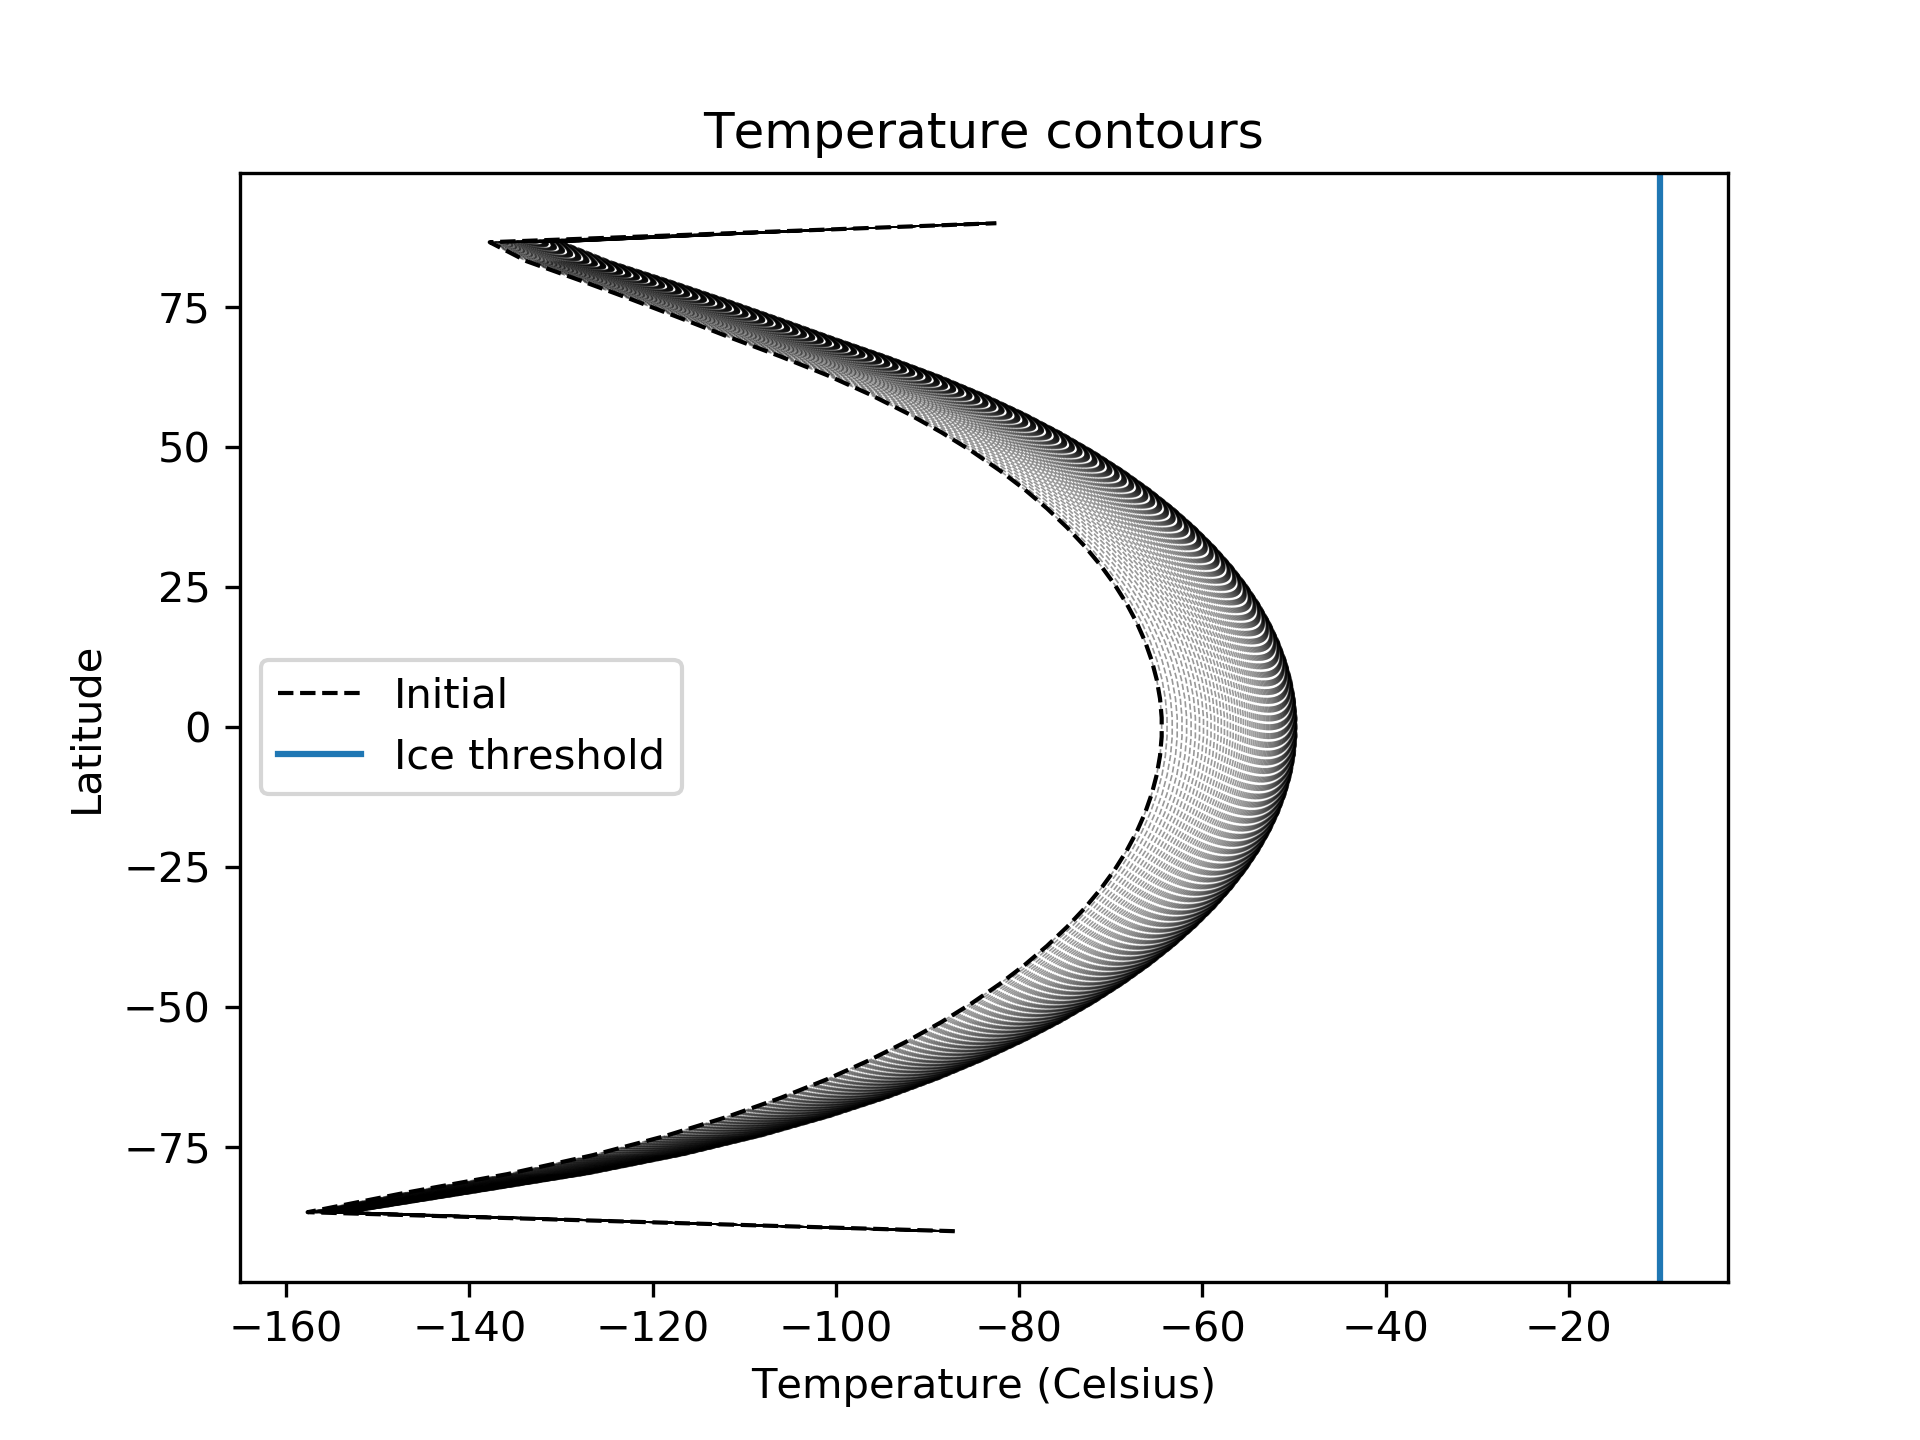
\includegraphics[scale=0.4]{tcont_58.png} 
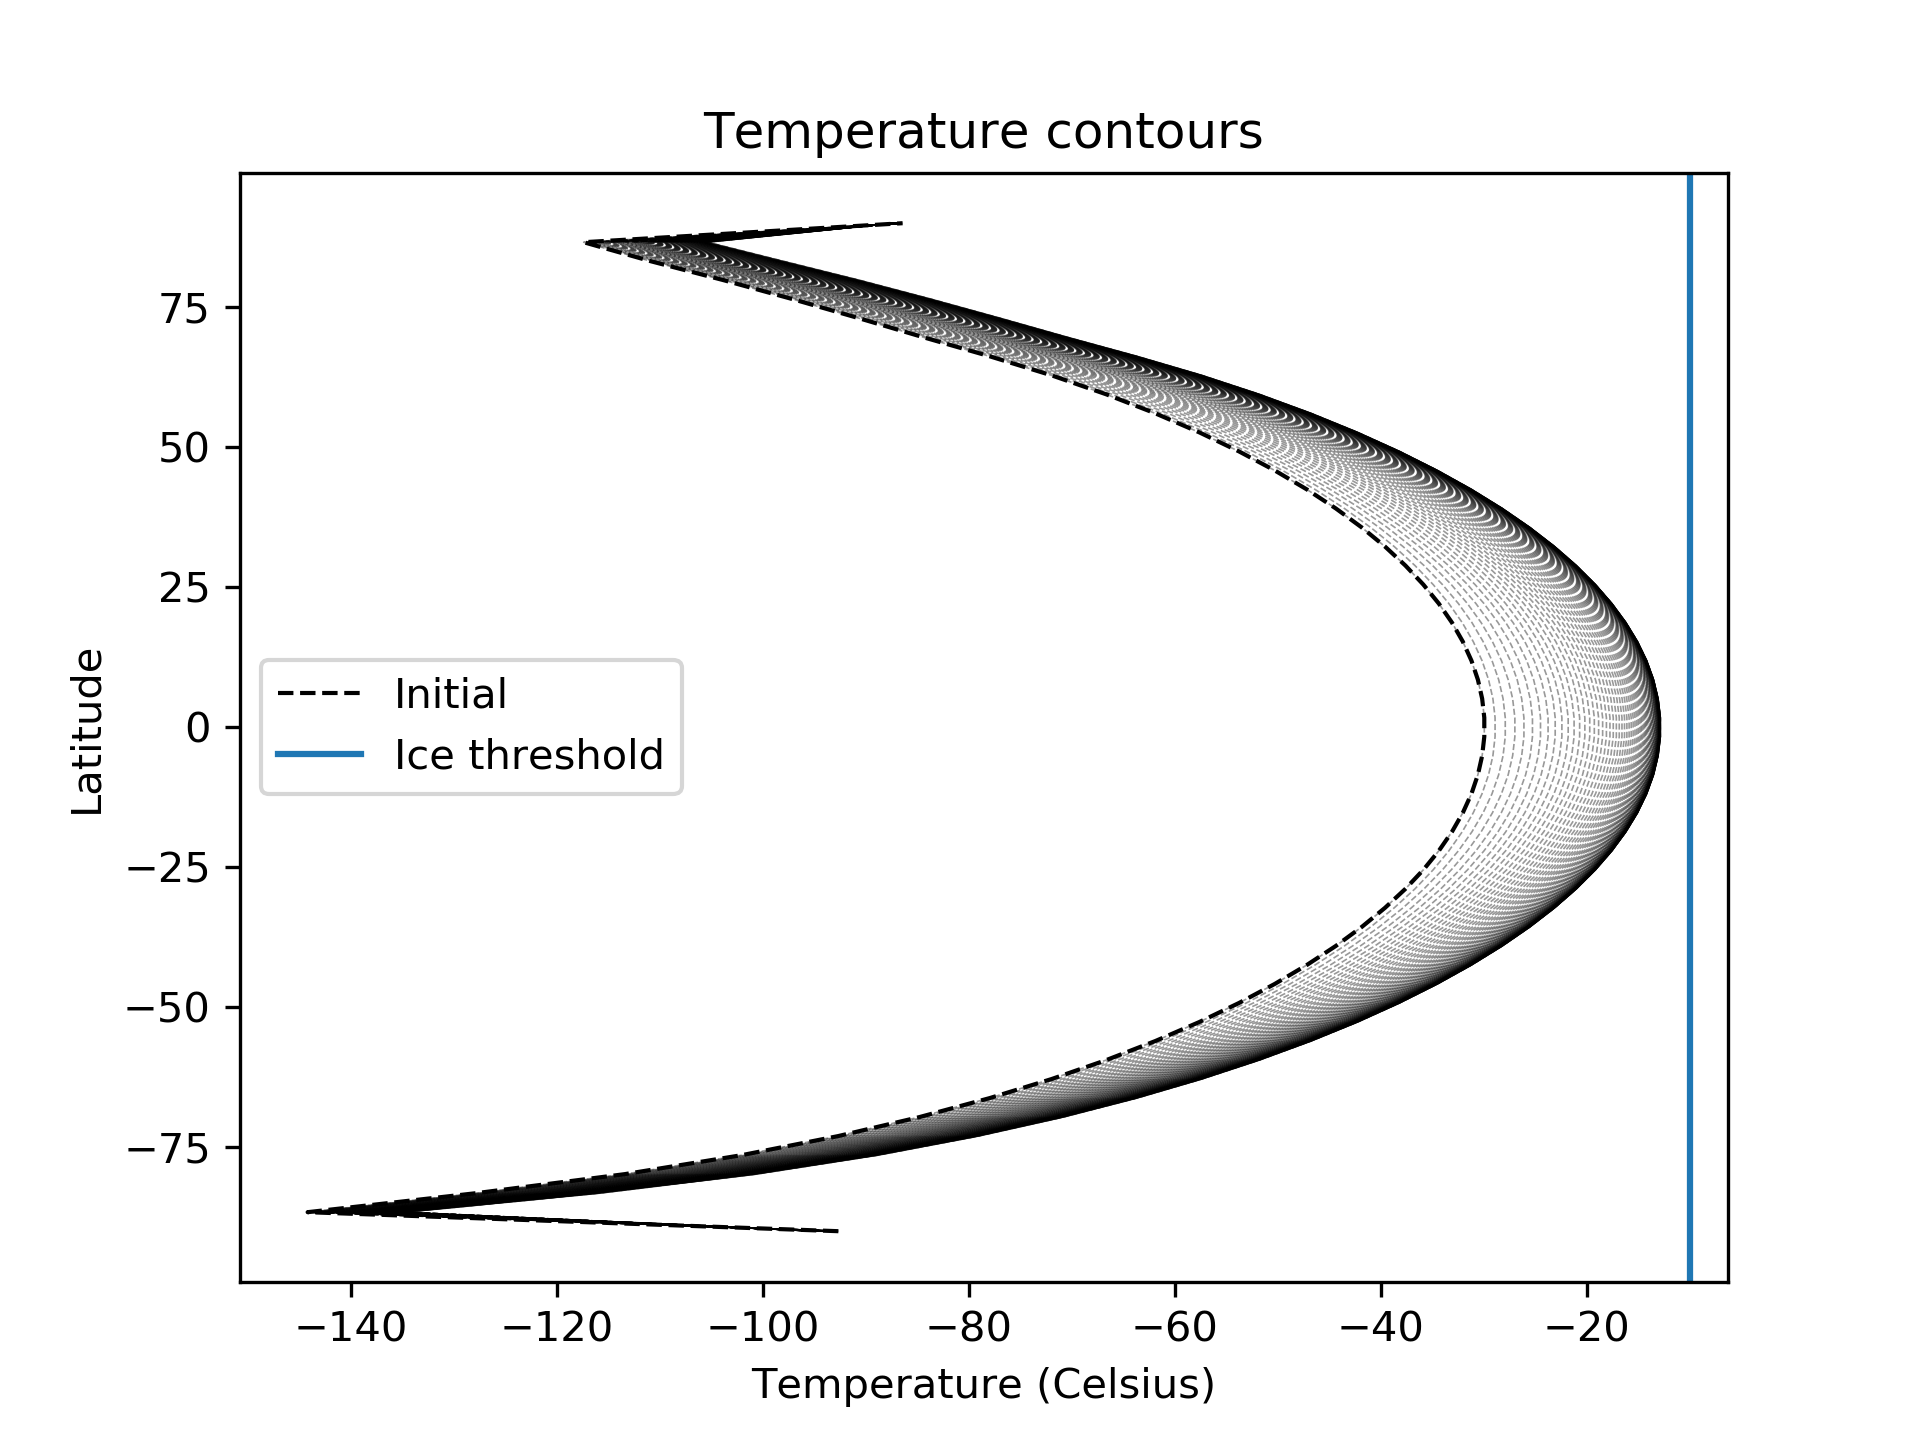
\includegraphics[scale=0.4]{tcont_510.png} 
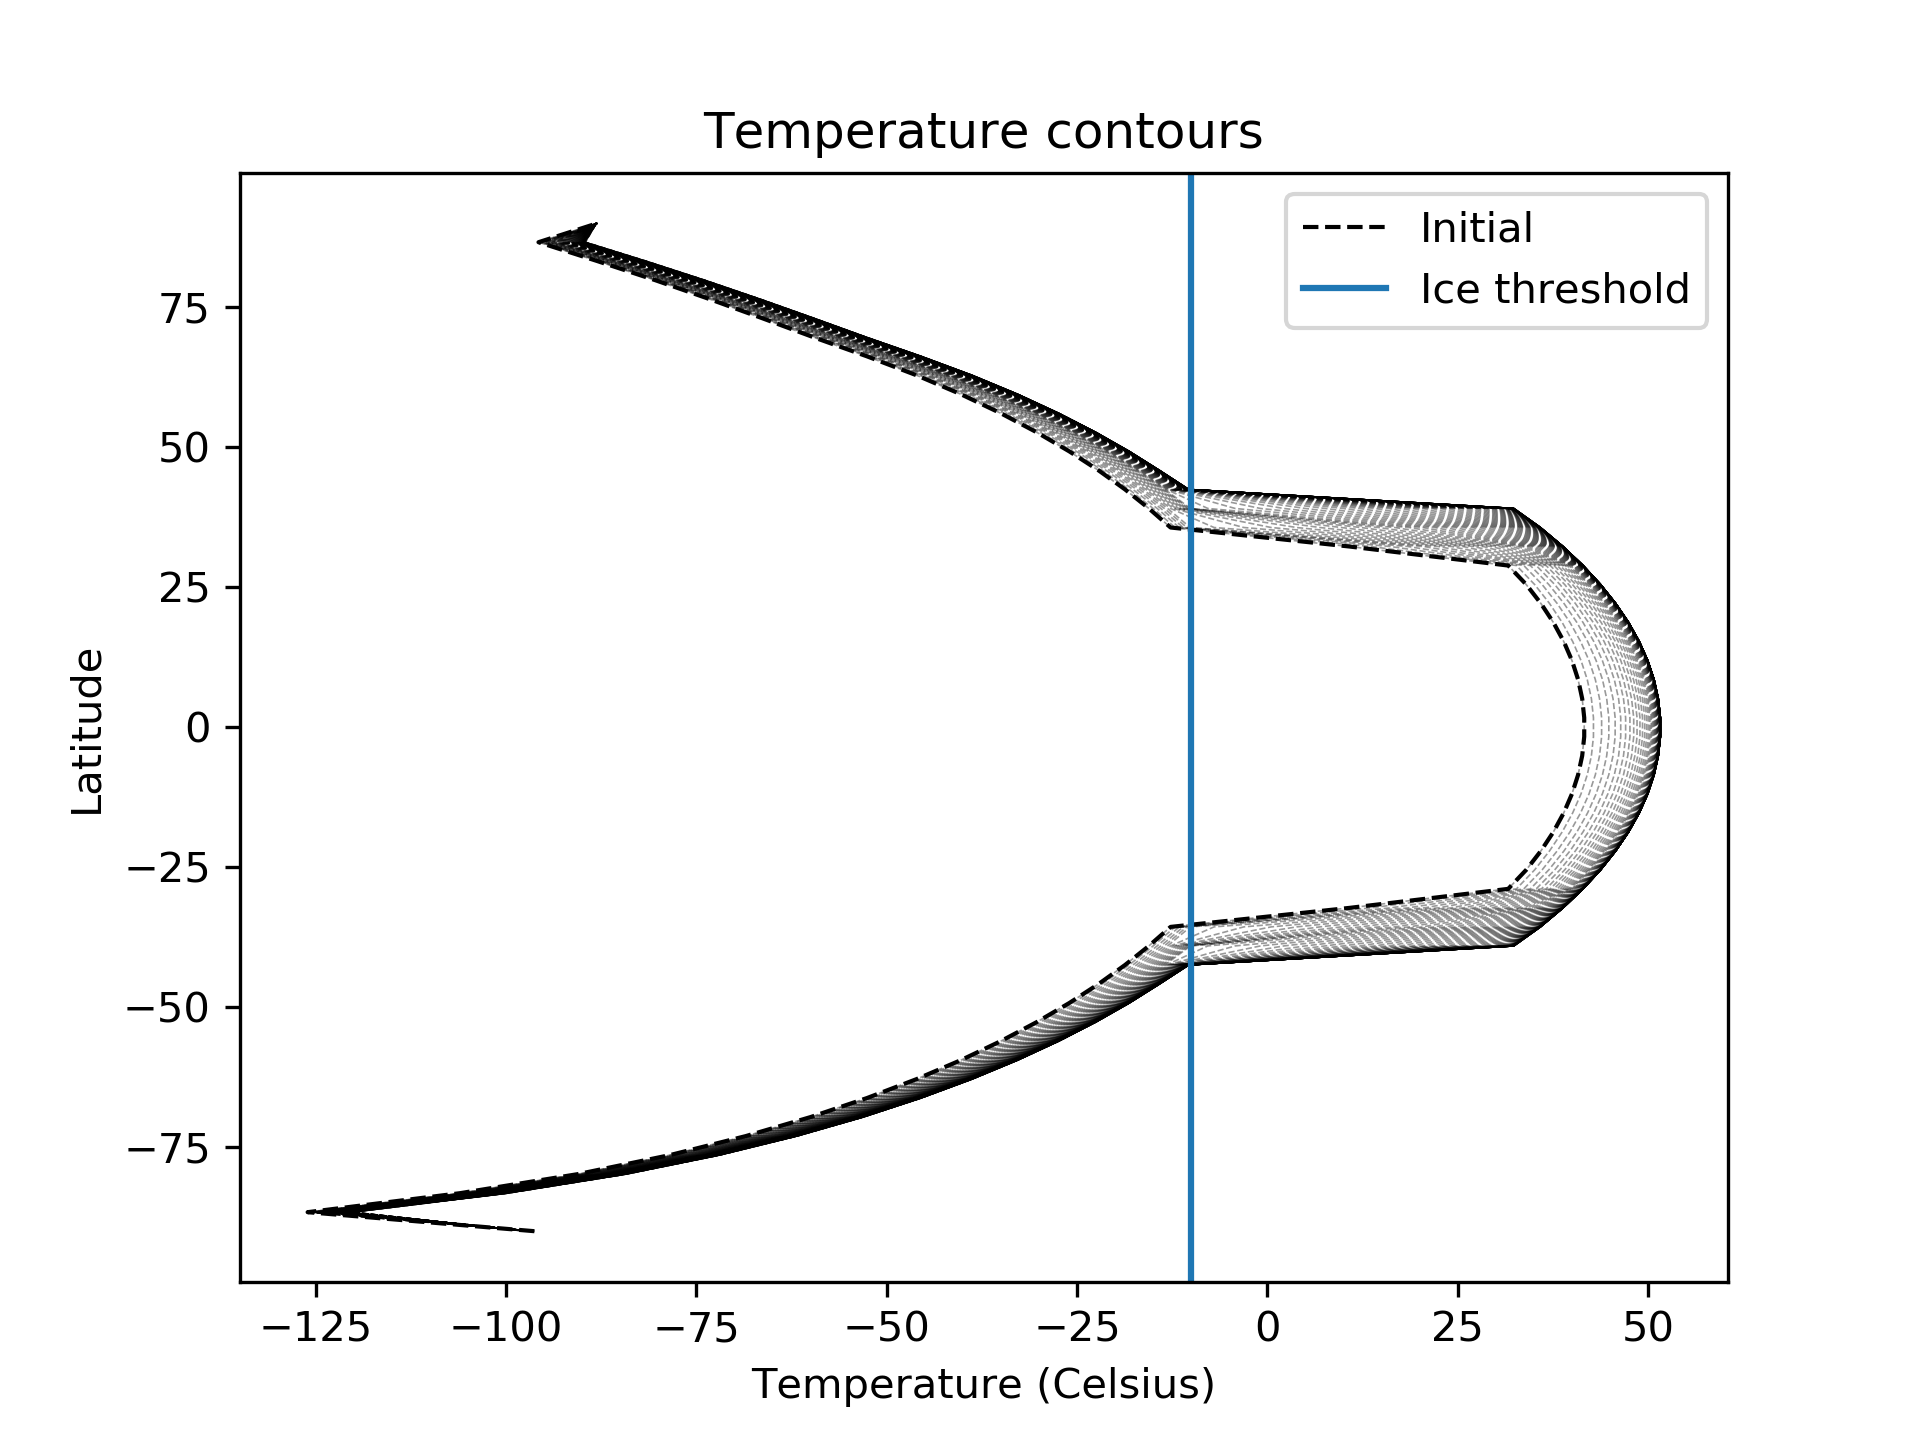
\includegraphics[scale=0.4]{tcont_512.png} 
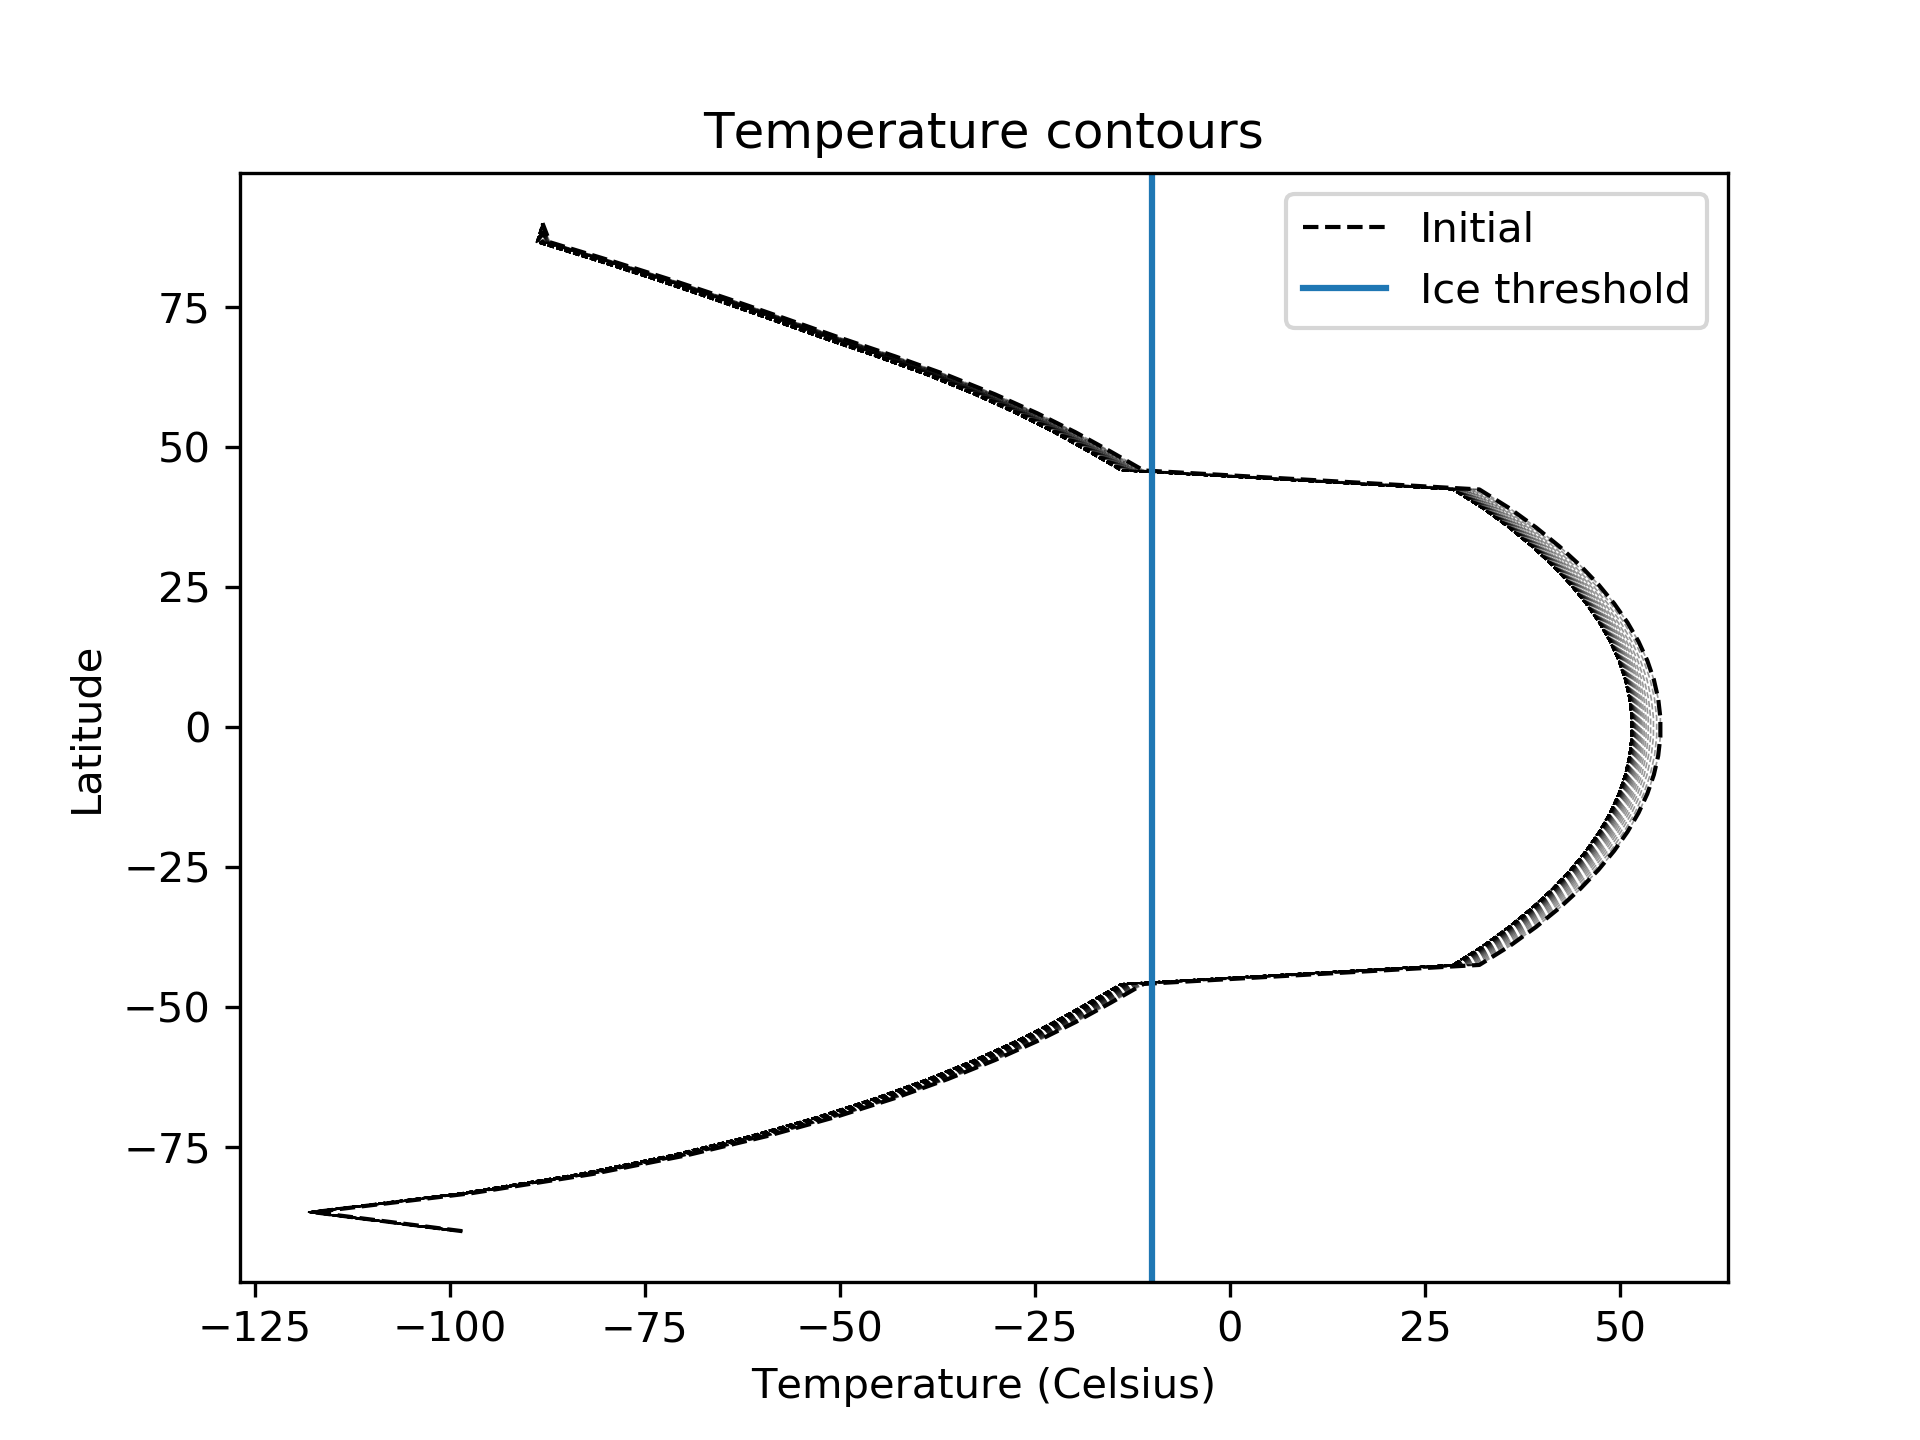
\includegraphics[scale=0.4]{tcont_514.png} 
\end{figure}
\begin{figure}
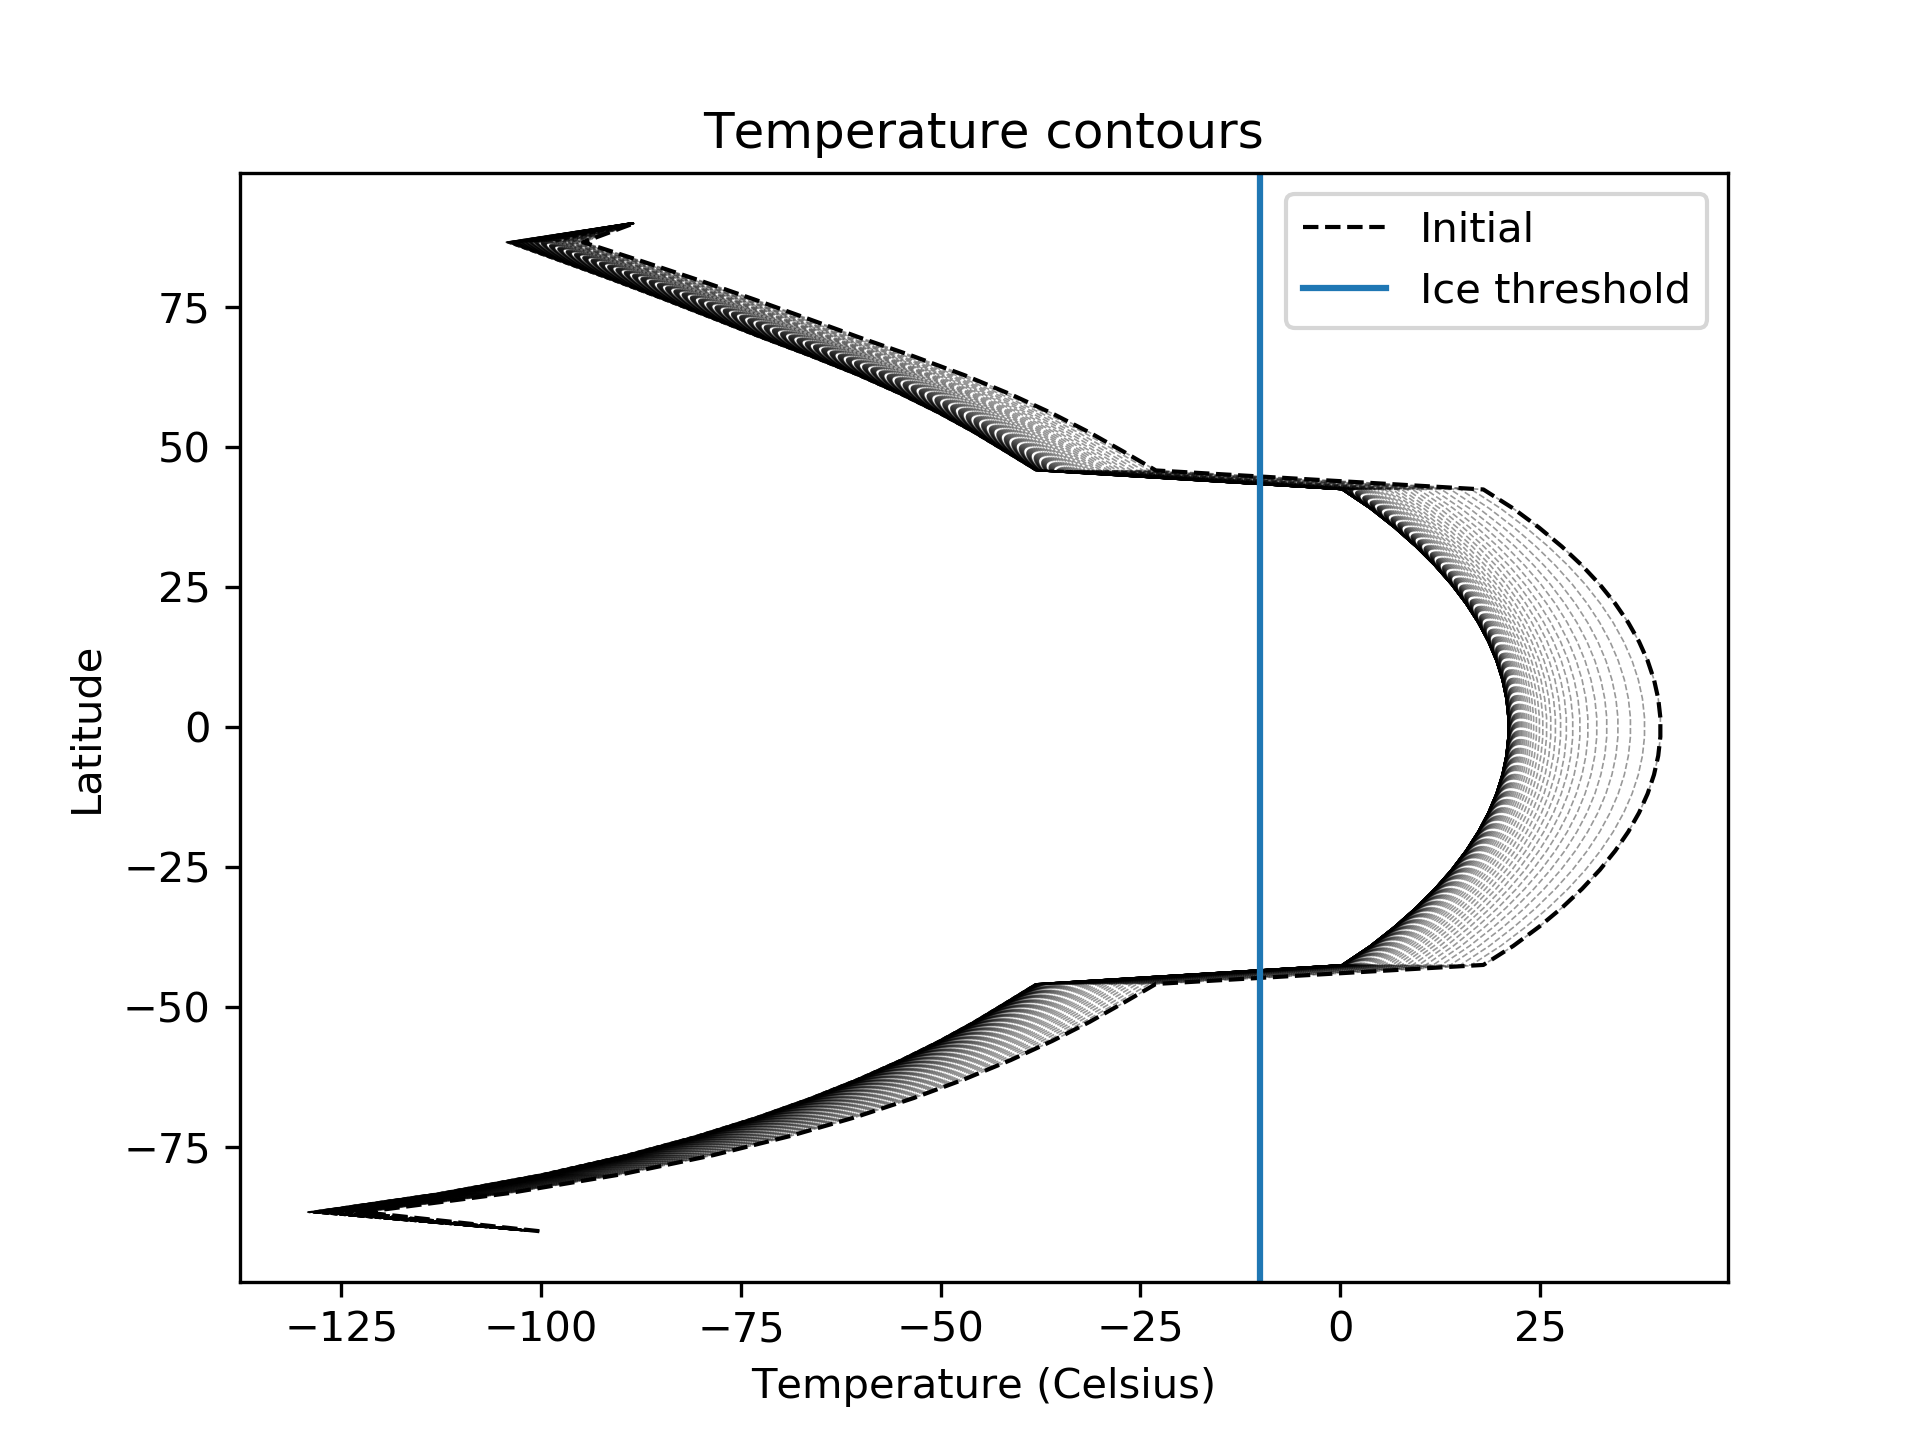
\includegraphics[scale=0.4]{tcont_516.png} 
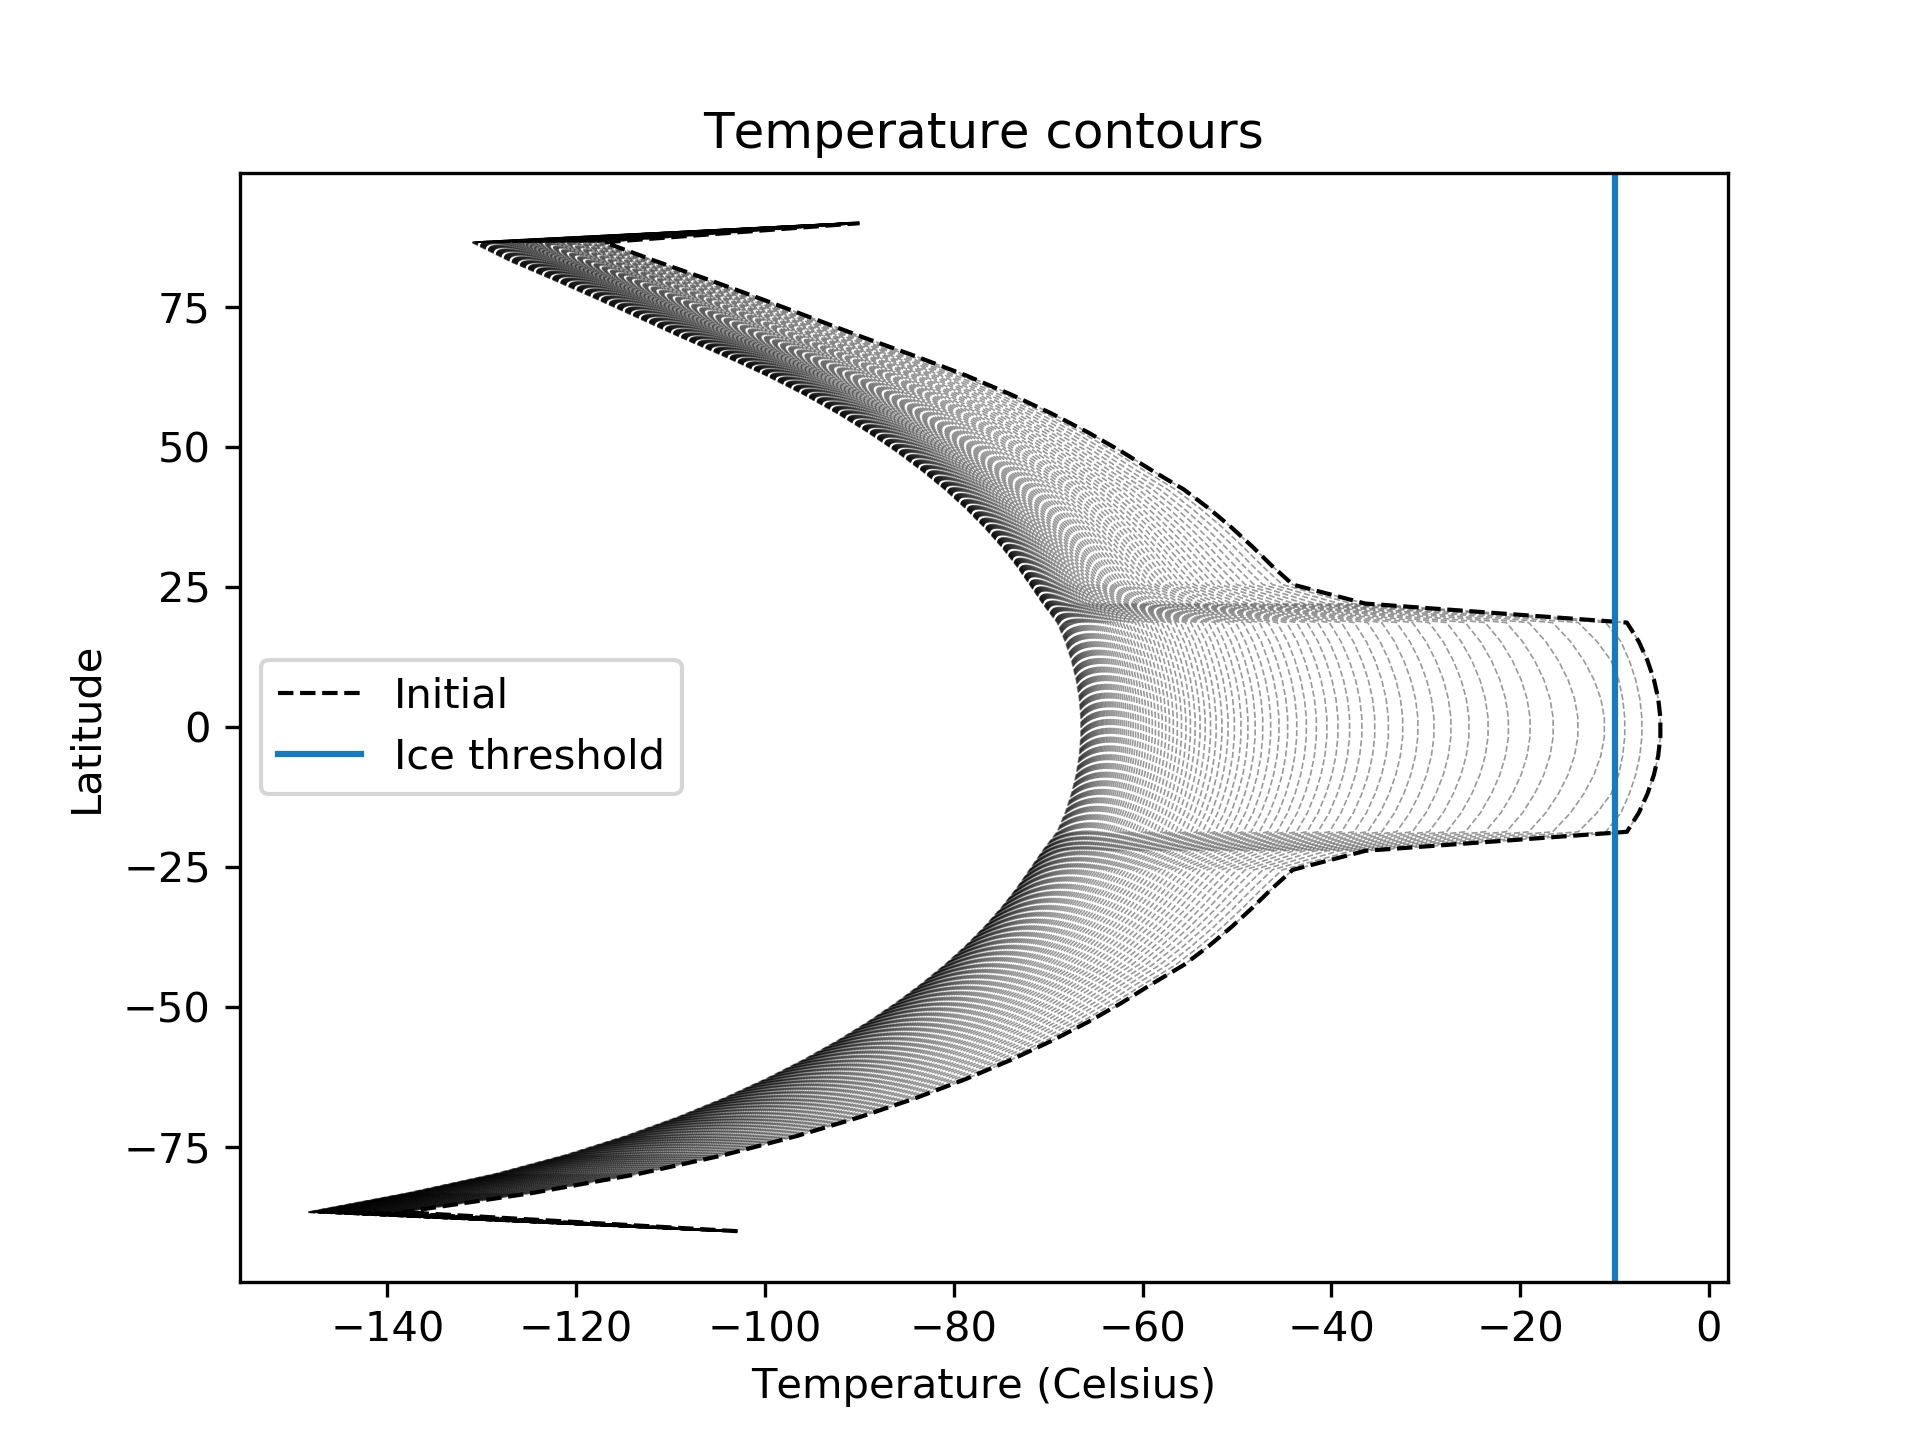
\includegraphics[scale=0.4]{tcont_518.png} 
\caption{Different simulations with varying solar intensity and initial temperature feedback.}
\end{figure}
\begin{figure}
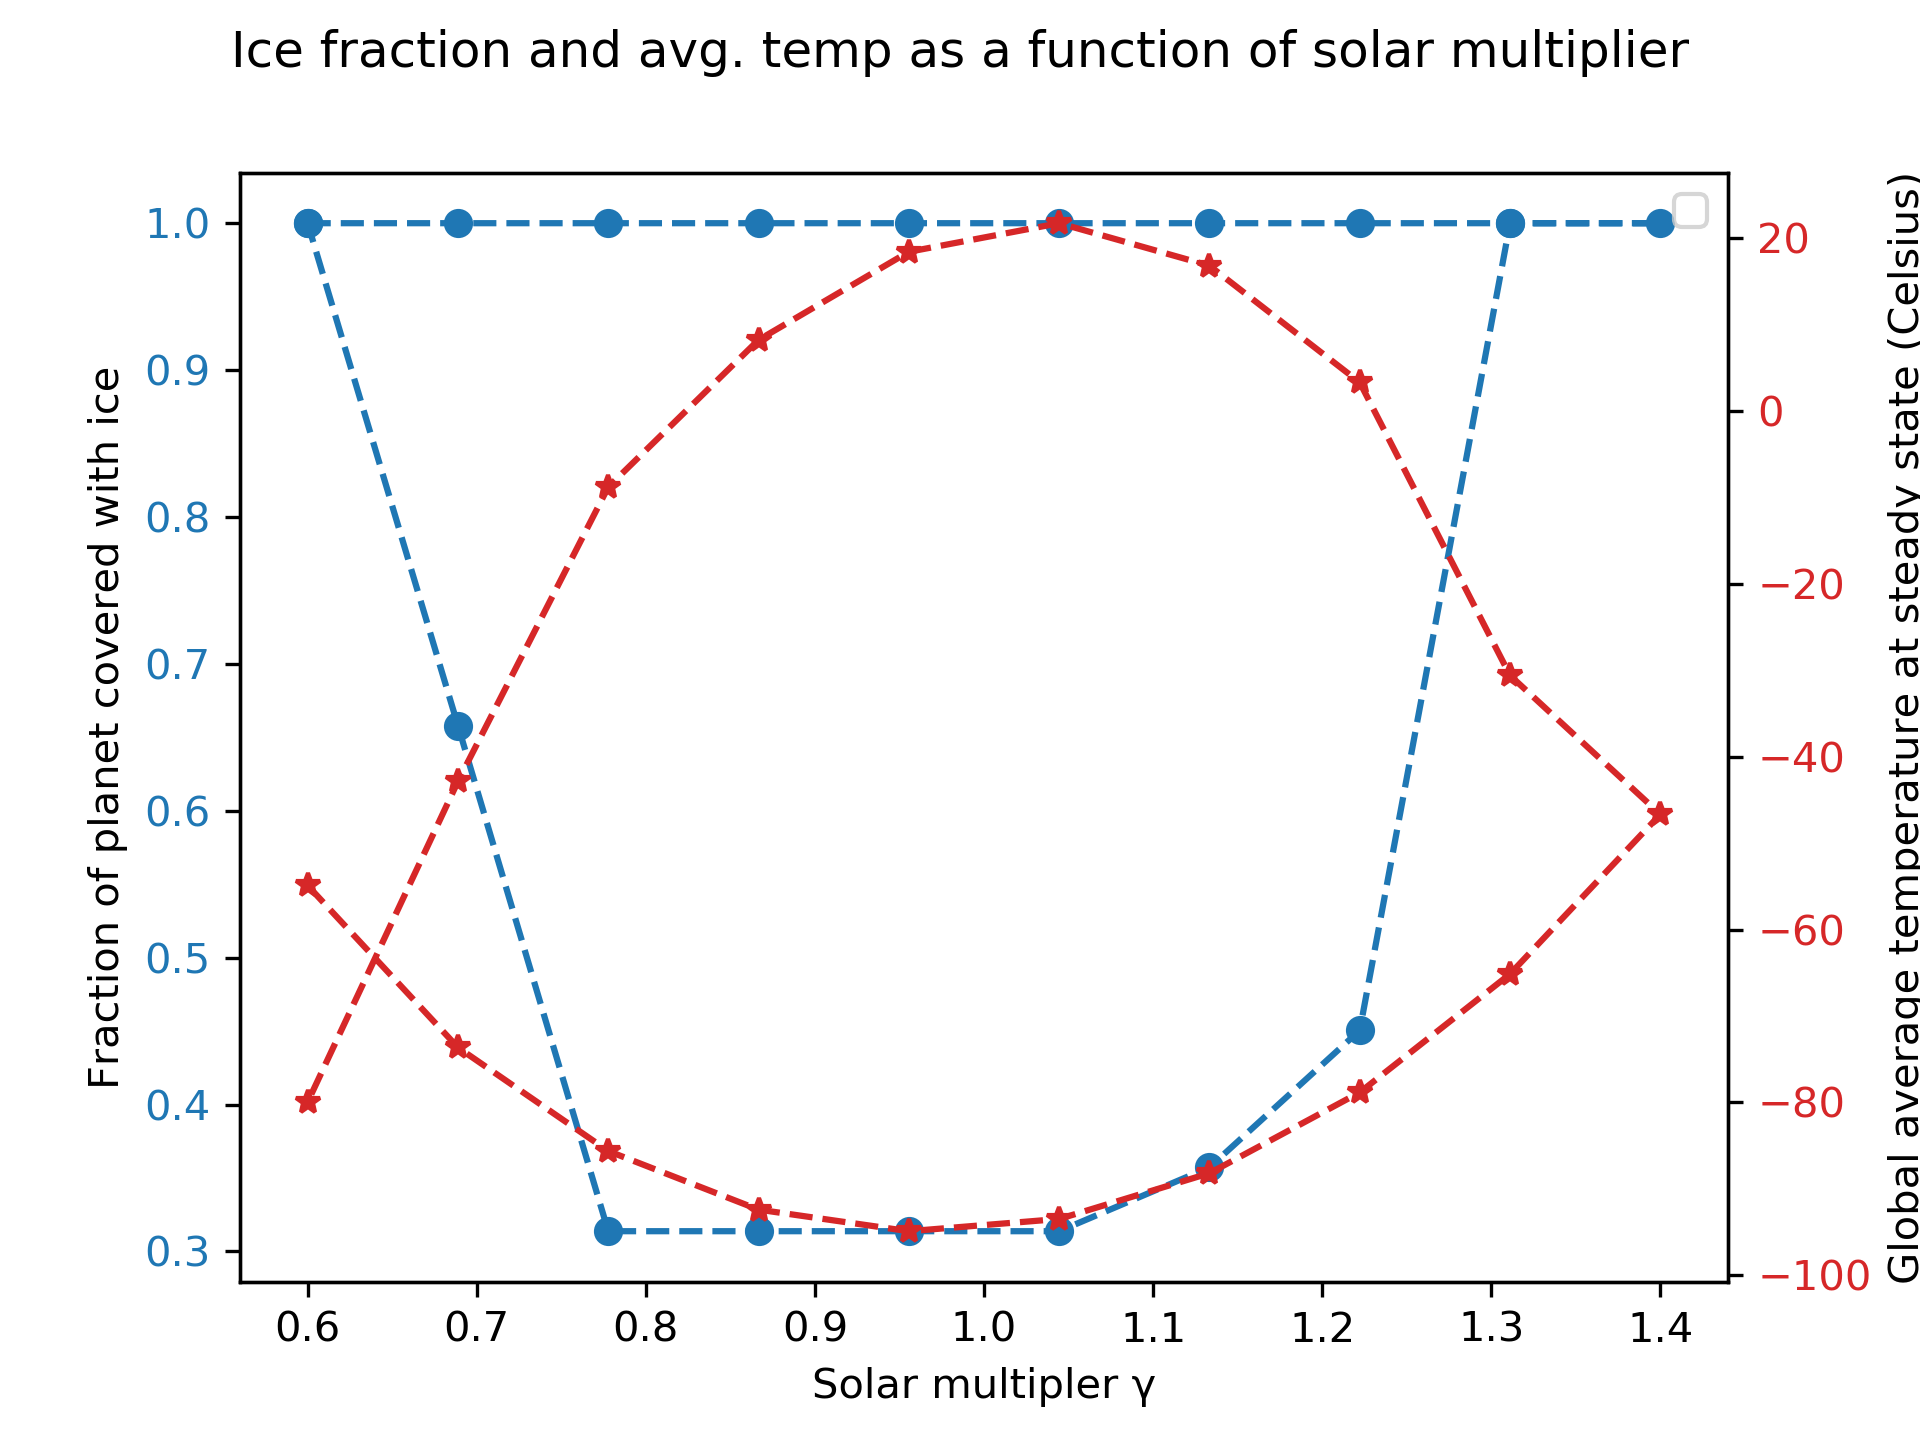
\includegraphics[scale=0.8]{ratios_5.png} 
\caption{Climate hysteresis:solar multiplier vs ice fraction and avg. temp.}
\end{figure}

\section*{Question 6}
$CO_2$ is a greenhouse gas which traps solar radiations. We could achieve $CO_2$ forcing in our system by increasing the emissivity of the atmosphere forcing in our system by increasing the emissivity of the atmosphere.

\section*{Question 7}
Assuming the initial temperature distribution to be same that in question 2, we have to reduce the solar intensity by 45\% , i.e., the $\gamma = 0.55$ for the entire planet to be covered in ice (Fig. 12). 
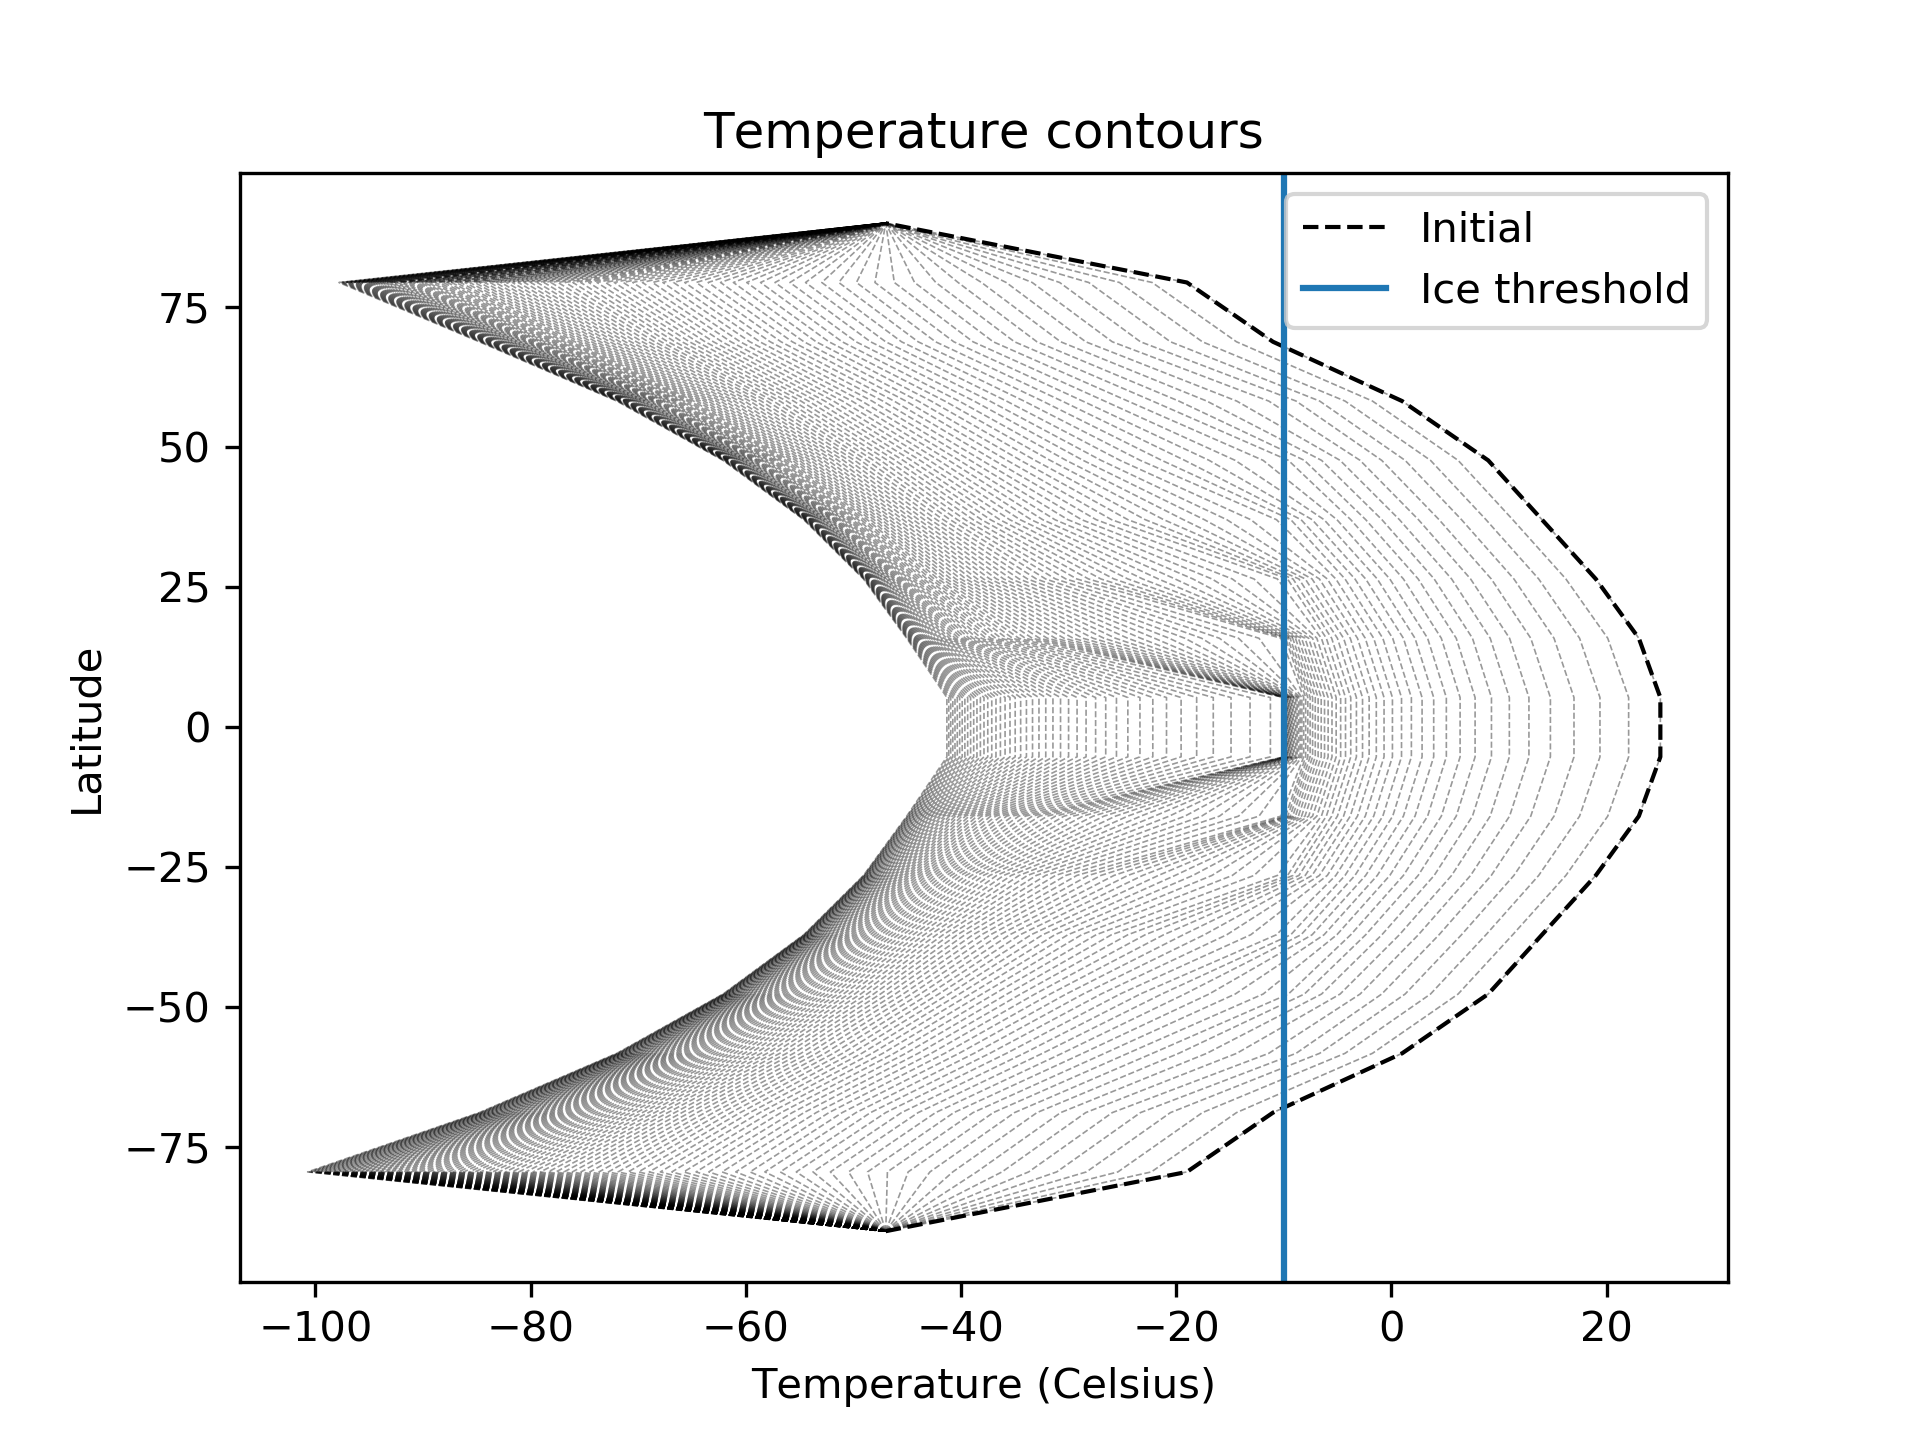
\includegraphics[scale=0.6]{tcont_70.png} 

\section*{Question 8}
Given the current temperature distribution as in question 2, the earth can never be completely ice free just by increasing the solar radiation. The fraction of ice stops decreasing after reaching the value of 0.152. The poles are always at ice.

\end{document}
